%\UseRawInputEncoding
\newif\ifcomments
\commentstrue % Use this version to allow in-draft comments
%\commentsfalse % Use this version to suppress comments

\documentclass[letterpaper,12pt,dvipsnames,usenames]{article}
\usepackage[latin1]{inputenc}
\usepackage{rotate}
\usepackage{rotating}
\usepackage{siunitx}
%\usepackage{xstring}
\usepackage{amsmath}
\usepackage{amssymb}
\usepackage{amsthm}
\usepackage{amsfonts}
%\usepackage{changepage}
\usepackage{booktabs}
\usepackage{caption}
\usepackage{subcaption}
\usepackage{setspace}
\usepackage{graphicx}
\DeclareGraphicsExtensions{.png,.eps}
\usepackage{mathpazo}
\usepackage[margin=1in]{geometry}
%\usepackage{tabu}
\usepackage[colorlinks=true, allcolors=BrickRed]{hyperref}
\usepackage[longnamesfirst]{natbib}
%\usepackage[capposition=top]{floatrow}
%\usepackage{subfig}

\newcommand{\sumn}{\sum_{i=1}^{n}}
\newcommand{\sumt}{\sum_{t=0}^\infty}
\newcommand{\sums}{\sum_{t=0}^\infty \sum_{s^t}}
\newcommand{\sumj}{\sum_{j=-\infty}^\infty}
\newcommand{\fsum}{\frac{1}{n} \sum_{i=1}^n}
\newcommand{\prodn}{\prod_{i=1}^{n}}
\newcommand{\intf}{\int_{-\infty}^{\infty}}
\newcommand{\intz}{\int_0^\infty}
\newcommand{\limf}{\lim_{n\to \infty}}
\newcommand{\I}{\mathbb{I}}
\newcommand{\N}{\mathbb{N}}
\newcommand{\R}{\mathbb{R}}
\newcommand{\E}{\mathbb{E}}
\newcommand{\Z}{\mathbb{Z}}
\newcommand{\C}{\mathbb{C}}
\newcommand{\M}{\mathcal{M}}
\newcommand{\bp}{\mathbb{P}}
\newcommand{\F}{\mathcal{F}}
\newcommand{\PP}{\mathbb{P}}
\newcommand{\Cost}{\text{Cost}}
%\newcommand{\pay}{\text{pay}}
\newcommand{\cH}{\mathcal{H}}
\newcommand{\Var}{\text{Var}}
\newcommand{\Cov}{\text{Cov}}
\newcommand{\topr}{\xrightarrow{  p  }}
\newcommand{\tod}{\xrightarrow{  d  }}
\newcommand{\blambda}{\bar{\lambda}}
\newcommand{\htheta}{\hat{\theta}}
\newcommand{\hbeta}{\hat{\beta}}
\newcommand{\hmu}{\hat{\mu}}
\newcommand{\hF}{\hat{F}}
\newcommand{\sss}{\subsubsection*}
\newcommand{\simiid}{\stackrel{\text{iid}}{\sim}}
\newcommand{\eqas}{\stackrel{\text{a.s.}}{=}}
\newcommand{\eps}{\varepsilon}
\newcommand{\re}{\text{Re}}
\newcommand{\im}{\text{Im}}
\newcommand{\cond}{ \; \Bigr| \; }
\newcommand{\maxtil}{ \widetilde{\max} }

\newcommand{\dxdy}[2]{\frac{\partial #1}{\partial #2}}
\newcommand{\ind}[1]{\mathbf{1}_{\{ #1 \} }}
\newcommand{\til}[1]{\tilde{#1}}

\newcommand{\pbrac}[1]{\left( #1 \right)}
\newcommand{\Bigpbrac}[1]{\Bigl( #1 \Bigr)}
\newcommand{\Biggpbrac}[1]{\Biggl( #1 \Biggr)}
\newcommand{\bigpbrac}[1]{\bigl( #1 \bigr)}
\newcommand{\biggpbrac}[1]{\biggl( #1 \biggr)}

\newcommand{\sbrac}[1]{\left[ #1 \right]}
\newcommand{\Bigsbrac}[1]{\Bigl[ #1 \Bigr]}
\newcommand{\Biggsbrac}[1]{\Biggl[ #1 \Biggr]}
\newcommand{\bigsbrac}[1]{\bigl[ #1 \bigr]}
\newcommand{\biggsbrac}[1]{\biggl[ #1 \biggr]}

\newcommand{\cbrac}[1]{\left\{ #1 \right\}}
\newcommand{\Bigcbrac}[1]{\Bigl\{ #1 \Bigr\}}
\newcommand{\biggcbrac}[1]{\biggl\{ #1 \biggr\}}
\newcommand{\bigcbrac}[1]{\bigl\{ #1 \bigr\}}
\newcommand{\Biggcbrac}[1]{\Biggl\{ #1 \Biggr\}}

\newcommand{\comment}[1]{\ifcomments {\color{red} [#1]} \fi}

\newcommand{\pfrac}[2]{\pbrac{\frac{#1}{#2}}}

\newcommand{\undertext}[2]{\underbrace{#1}_{\text{#2}}}

%\newcommand{\absoluteone}[1]{\if\StrBehind[1]{#1}{-}\empty #1 \else \StrBehind[1]{#1}{-} \fi}
%\newcommand{\absolute}[1]{%
%   \begingroup\edef\x{\endgroup\noexpand\absoluteone{#1}}\x
%}

\newcommand{\calsection}[1]{\midrule \multicolumn{4}{c}{\textit{#1}} \\ \midrule}
\newcommand{\tabsection}[2]{\midrule \multicolumn{#1}{c}{\textit{#2}} \\ \midrule}
\newenvironment{figurenotes}{\begin{spacing}{1.0} \footnotesize \emph{Note:} }{\end{spacing}}

\newcommand{\readmoments}[2]{& \input{#2/mean/#1.tex} & \input{#2/std/#1.tex}}
\newcommand{\allmoments}[1]{& \readmoments{#1}{\dira} & \readmoments{#1}{\dirb} & \readmoments{#1}{\dirc}}

\def\resversion{20171109}
\def\texdir{../Code/version\resversion/tex}
\def\caldir{\texdir/cal}
\newcommand{\readcal}[1]{\input{\caldir/#1.tex}\unskip}
\newcommand{\readcalpct}[1]{\input{\caldir/#1_pct.tex}\unskip\%}

\newcommand{\readval}[2]{\input{\texdir/xi_alt_#1/#2.tex}\unskip}
\newcommand{\baseval}[1]{\readval{no_index}{#1}}
\newcommand{\readvalNoXi}[2]{\input{\texdir/#1/#2.tex}\unskip}

\def\miscdir{\texdir/misc}
\newcommand{\readmisc}[1]{\input{\miscdir/#1.tex}\unskip}

\newcommand{\readvalrowNoXi}[2]{#1 & \readvalNoXi{no_index}{#2} & \readvalNoXi{agg}{#2} & \readvalNoXi{idio_25}{#2} & \readvalNoXi{idio_50}{#2} \\}
%\newcommand{\readvalrowxi}[2]{#1 & \readval{xi_no_index}{#2} & \readval{xi_agg}{#2} & \readval{xi_idio_25}{#2} & \readval{xi_idio_50}{#2} \\}
\newcommand{\readvalrow}[2]{#1 & \readval{no_index}{#2} & \readval{agg}{#2} & \readval{idio_25_only}{#2} & \readval{idio_25}{#2} \\}
%\newcommand{\readvalxx}[2]{\input{\texdir/#1/#2_val2.tex}\unskip}
%\newcommand{\readpct}[2]{\input{\texdir/#1/#2_pct.tex}\unskip\%}
%\newcommand{\readpctx}[2]{\input{\texdir/#1/#2_pct1.tex}\unskip\%}
%\newcommand{\readpctxx}[2]{\input{\texdir/#1/#2_pct3.tex}\unskip\%}

\newcommand{\para}[1]{\paragraph{#1.}}

\newcommand{\mbs}[1]{\boldsymbol{#1}}
\newcommand{\Tau}{\mathcal{T}}

\allowdisplaybreaks[1]

%\numberwithin{equation}{section}

\theoremstyle{definition}
\newtheorem{thm}{Theorem}
\newtheorem{claim}{Claim}
\newtheorem{prop}[thm]{Proposition}
\newtheorem{defn}{Definition}
\newtheorem{cor}{Corollary}
\newtheorem{ex}{Example}
\newtheorem{exer}{Exercise}
\newtheorem{lem}[thm]{Lemma}
\newtheorem{ob}{Observation}
\newtheorem{fact}{Fact}

%\linespread{1.6}
\linespread{1.3}







%------------------------------------------------------
% DEFINE NUMERICAL RESULTS HERE
%------------------------------------------------------

\def\calPhiK{85\%}

\newcommand{\IncStates}{0.258 0.775 2.192}
\newcommand{\psiz}{0.461 1.063 1.413}
\newcommand{\taxss}{0.10}
\newcommand{\PbetaL}{0.793}
\newcommand{\PbetaH}{1.020}
\newcommand{\Pgamma}{ 5.0}
\newcommand{\alphaC}{0.74}
\newcommand{\alphaH}{0.26}
\newcommand{\alphaN}{0.68}
\newcommand{\ElastCN}{0.00}
\newcommand{\ElastCH}{-0.50}
\newcommand{\HoursMinbyHours}{0.15}
\newcommand{\Ptheta}{1.15}
\newcommand{\PQ}{0.825}
\newcommand{\Pkappa}{0.90}
\newcommand{\thetaRes}{0.90}
\newcommand{\thetaInv}{0.90}
\newcommand{\tauP}{6.30}
\newcommand{\deprH}{0.0946}
\newcommand{\HresMinbyHresRatio}{0.45}
\newcommand{\RTSC}{0.66}
\newcommand{\HBARone}{0.21}
\newcommand{\HBARtwo}{3.30}
\newcommand{\PphiT}{0.036}
\newcommand{\PphiF}{0.033}
\newcommand{\OOTElas}{ 0.6}
\newcommand{\OOTLevel}{-5.027 -4.250}
\newcommand{\Ppi}{0.90}
\newcommand{\PchiAll}{0.93}
\newcommand{\PchiW}{1.03}
\newcommand{\PchiR}{1.05}
\newcommand{\Pchibar}{0.25}
\newcommand{\fracRet}{21.9}
\newcommand{\HoursMinBind}{21.90}
\newcommand{\taxssper}{  10}
\newcommand{\Ppsizone}{0.46}
\newcommand{\Ppsiztwo}{1.06}
\newcommand{\Ppsizthree}{1.41}
\newcommand{\RetInc}{26,914}
\newcommand{\RetIncbyLabInc}{35.84}
\newcommand{\AvgHours}{30.6}
\newcommand{\HousTotConsratio}{25.2}
\newcommand{\FrischEMacro}{1.03}
\newcommand{\FrischEMicro}{1.16}
\newcommand{\PbetaLy}{0.944}
\newcommand{\PbetaHy}{1.005}
\newcommand{\Pbeta}{0.85}
\newcommand{\NWbyInc}{5.87}
\newcommand{\GiniNW}{0.78}
\newcommand{\Probbequest}{ 9.5}
\newcommand{\fracbeqann}{ 1.8}
\newcommand{\PchiAllchiR}{0.98}
\newcommand{\fracRetRel}{0.84}
\newcommand{\IncRel}{1.12}
\newcommand{\MedMktRentbySqftRel}{1.03}
\newcommand{\HORel}{0.45}
\newcommand{\cbarFrac}{30.7}
\newcommand{\HSE}{0.94}
\newcommand{\HSEone}{0.45}
\newcommand{\HSEtwo}{0.99}
\newcommand{\HoverHbar}{0.16}
\newcommand{\HbaroneDist}{50.8}
\newcommand{\HbartwoDist}{85.9}
\newcommand{\tauPy}{1.58}
\newcommand{\ImInt}{4.93}
\newcommand{\MedMktPHbyMedMktRent}{13.02}
\newcommand{\HresMin}{720}
\newcommand{\HresMinbyHres}{45.1}
\newcommand{\CommCost}{ 3.6}
\newcommand{\CommCostFinDollar}{2,478}
\newcommand{\CommCostFinbyInc}{ 3.3}
\newcommand{\AvgOwnRate}{63.4}
\newcommand{\AvgOwnRateA}{64.7}
\newcommand{\AvgOwnRateB}{62.8}
\newcommand{\GiniInc}{0.43}
\newcommand{\BaselineWelP}{0.61}
\newcommand{\BaselineWelRP}{2.02}
\newcommand{\BaselineWelOP}{0.43}
\newcommand{\BaselineAgeTwoOwnHurt}{ 5.1}
\newcommand{\BaselineAgeForteenOwnHurt}{28.1}
\newcommand{\BaselineAvgBenefit}{  55}
\newcommand{\BaselineAvgOwnBenefit}{  84}
\newcommand{\BaselineAvgRentBenefit}{   5}
\newcommand{\TaxbyInc}{ 4.7}
\newcommand{\ZOneHIncrease}{13.5}
\newcommand{\NWMidChZoneOne}{21.0}
\newcommand{\WageMidChZoneOne}{ 5.4}
\newcommand{\OwnLocalChangeZoneOne}{ 4.8}
\newcommand{\OwnLocalChangeZoneTwo}{ 1.1}
\newcommand{\SizeChShort}{-0.1}
\newcommand{\SizeChLong}{ 2.5}
\newcommand{\WageChShort}{ 0.6}
\newcommand{\WageChLong}{ 0.4}
\newcommand{\FracConstructChShort}{17.6}
\newcommand{\FracConstructBefore}{ 5.6}
\newcommand{\FracConstructAfter}{ 6.6}
\newcommand{\HoursWorkedChange}{ 0.7}
\newcommand{\EarningsChange}{0.08}
\newcommand{\OwnerHCChange}{ 3.7}
\newcommand{\OwnerOCChange}{ 0.7}
\newcommand{\BaselineAgeFourtyWelR}{0.86}
\newcommand{\BaselineAgeSeventyFiveWelR}{9.42}
\newcommand{\BaselineAgeFourtyWelO}{0.62}
\newcommand{\BaselineAgeNinetyFiveWelO}{1.99}

\newcommand{\BaselineW}[2]{\ifnum #2=1 \num[round-mode=places,round-precision=#1]{0.5929} \else \num[round-mode=places,round-precision=#1]{0.5929}\fi}
\newcommand{\BaselineRone}[2]{\ifnum #2=1 \num[round-mode=places,round-precision=#1]{10.9617} \else \num[round-mode=places,round-precision=#1]{10.9617}\fi}
\newcommand{\BaselineRtwo}[2]{\ifnum #2=1 \num[round-mode=places,round-precision=#1]{10.6756} \else \num[round-mode=places,round-precision=#1]{10.6756}\fi}
\newcommand{\BaselinePone}[2]{\ifnum #2=1 \num[round-mode=places,round-precision=#1]{6.5441} \else \num[round-mode=places,round-precision=#1]{6.5441}\fi}
\newcommand{\BaselinePtwo}[2]{\ifnum #2=1 \num[round-mode=places,round-precision=#1]{6.2693} \else \num[round-mode=places,round-precision=#1]{6.2693}\fi}
\newcommand{\BaselineINVone}[2]{\ifnum #2=1 \num[round-mode=places,round-precision=#1]{9.2014} \else \num[round-mode=places,round-precision=#1]{9.2014}\fi}
\newcommand{\BaselineINVtwo}[2]{\ifnum #2=1 \num[round-mode=places,round-precision=#1]{10.8323} \else \num[round-mode=places,round-precision=#1]{10.8323}\fi}
\newcommand{\BaselinePoneByRone}[2]{\ifnum #2=1 \num[round-mode=places,round-precision=#1]{3.9781} \else \num[round-mode=places,round-precision=#1]{-3.9781}\fi}
\newcommand{\BaselinePtwoByRtwo}[2]{\ifnum #2=1 \num[round-mode=places,round-precision=#1]{3.9791} \else \num[round-mode=places,round-precision=#1]{-3.9791}\fi}
\newcommand{\BaselineHPoneByY}[2]{\ifnum #2=1 \num[round-mode=places,round-precision=#1]{13.8581} \else \num[round-mode=places,round-precision=#1]{13.8581}\fi}
\newcommand{\BaselineHPtwoByY}[2]{\ifnum #2=1 \num[round-mode=places,round-precision=#1]{4.2920} \else \num[round-mode=places,round-precision=#1]{4.2920}\fi}
\newcommand{\BaselineHRoneByY}[2]{\ifnum #2=1 \num[round-mode=places,round-precision=#1]{18.5767} \else \num[round-mode=places,round-precision=#1]{18.5767}\fi}
\newcommand{\BaselineHRtwoByY}[2]{\ifnum #2=1 \num[round-mode=places,round-precision=#1]{8.6145} \else \num[round-mode=places,round-precision=#1]{8.6145}\fi}
\newcommand{\BaselineOwn}[2]{\ifnum #2=1 \num[round-mode=places,round-precision=#1]{3.0623} \else \num[round-mode=places,round-precision=#1]{3.0623}\fi}
\newcommand{\BaselineZoneOneFrac}[2]{\ifnum #2=1 \num[round-mode=places,round-precision=#1]{0.1685} \else \num[round-mode=places,round-precision=#1]{-0.1685}\fi}
\newcommand{\BaselineZoneTwoFrac}[2]{\ifnum #2=1 \num[round-mode=places,round-precision=#1]{0.1278} \else \num[round-mode=places,round-precision=#1]{0.1278}\fi}
\newcommand{\BaselineWel}[2]{\ifnum #2=1 \num[round-mode=places,round-precision=#1]{0.6070} \else \num[round-mode=places,round-precision=#1]{-0.6070}\fi}
\newcommand{\BaselineWelR}[2]{\ifnum #2=1 \num[round-mode=places,round-precision=#1]{2.0214} \else \num[round-mode=places,round-precision=#1]{-2.0214}\fi}
\newcommand{\BaselineWelO}[2]{\ifnum #2=1 \num[round-mode=places,round-precision=#1]{0.4254} \else \num[round-mode=places,round-precision=#1]{0.4254}\fi}
\newcommand{\BaselineSSW}[2]{\ifnum #2=1 \num[round-mode=places,round-precision=#1]{0.3560} \else \num[round-mode=places,round-precision=#1]{0.3560}\fi}
\newcommand{\BaselineSSRone}[2]{\ifnum #2=1 \num[round-mode=places,round-precision=#1]{8.7465} \else \num[round-mode=places,round-precision=#1]{8.7465}\fi}
\newcommand{\BaselineSSRtwo}[2]{\ifnum #2=1 \num[round-mode=places,round-precision=#1]{8.3858} \else \num[round-mode=places,round-precision=#1]{8.3858}\fi}
\newcommand{\BaselineSSPone}[2]{\ifnum #2=1 \num[round-mode=places,round-precision=#1]{4.9836} \else \num[round-mode=places,round-precision=#1]{4.9836}\fi}
\newcommand{\BaselineSSPtwo}[2]{\ifnum #2=1 \num[round-mode=places,round-precision=#1]{4.6912} \else \num[round-mode=places,round-precision=#1]{4.6912}\fi}
\newcommand{\BaselineSSINVone}[2]{\ifnum #2=1 \num[round-mode=places,round-precision=#1]{3.8673} \else \num[round-mode=places,round-precision=#1]{3.8673}\fi}
\newcommand{\BaselineSSINVtwo}[2]{\ifnum #2=1 \num[round-mode=places,round-precision=#1]{6.1771} \else \num[round-mode=places,round-precision=#1]{6.1771}\fi}
\newcommand{\BaselineSSPoneByRone}[2]{\ifnum #2=1 \num[round-mode=places,round-precision=#1]{3.4589} \else \num[round-mode=places,round-precision=#1]{-3.4589}\fi}
\newcommand{\BaselineSSPtwoByRtwo}[2]{\ifnum #2=1 \num[round-mode=places,round-precision=#1]{3.4082} \else \num[round-mode=places,round-precision=#1]{-3.4082}\fi}
\newcommand{\BaselineSSHPoneByY}[2]{\ifnum #2=1 \num[round-mode=places,round-precision=#1]{11.0366} \else \num[round-mode=places,round-precision=#1]{11.0366}\fi}
\newcommand{\BaselineSSHPtwoByY}[2]{\ifnum #2=1 \num[round-mode=places,round-precision=#1]{4.9259} \else \num[round-mode=places,round-precision=#1]{4.9259}\fi}
\newcommand{\BaselineSSHRoneByY}[2]{\ifnum #2=1 \num[round-mode=places,round-precision=#1]{15.0057} \else \num[round-mode=places,round-precision=#1]{15.0057}\fi}
\newcommand{\BaselineSSHRtwoByY}[2]{\ifnum #2=1 \num[round-mode=places,round-precision=#1]{8.6298} \else \num[round-mode=places,round-precision=#1]{8.6298}\fi}
\newcommand{\BaselineSSOwn}[2]{\ifnum #2=1 \num[round-mode=places,round-precision=#1]{2.7603} \else \num[round-mode=places,round-precision=#1]{2.7603}\fi}
\newcommand{\BaselineSSZoneOneFrac}[2]{\ifnum #2=1 \num[round-mode=places,round-precision=#1]{2.3694} \else \num[round-mode=places,round-precision=#1]{-2.3694}\fi}

\newcommand{\NoZoneTwoOOTW}[2]{\ifnum #2=1 \num[round-mode=places,round-precision=#1]{0.2369} \else \num[round-mode=places,round-precision=#1]{0.2369}\fi}
\newcommand{\NoZoneTwoOOTRone}[2]{\ifnum #2=1 \num[round-mode=places,round-precision=#1]{5.3024} \else \num[round-mode=places,round-precision=#1]{5.3024}\fi}
\newcommand{\NoZoneTwoOOTRtwo}[2]{\ifnum #2=1 \num[round-mode=places,round-precision=#1]{4.2779} \else \num[round-mode=places,round-precision=#1]{4.2779}\fi}
\newcommand{\NoZoneTwoOOTPone}[2]{\ifnum #2=1 \num[round-mode=places,round-precision=#1]{3.3640} \else \num[round-mode=places,round-precision=#1]{3.3640}\fi}
\newcommand{\NoZoneTwoOOTPtwo}[2]{\ifnum #2=1 \num[round-mode=places,round-precision=#1]{2.6417} \else \num[round-mode=places,round-precision=#1]{2.6417}\fi}
\newcommand{\NoZoneTwoOOTINVone}[2]{\ifnum #2=1 \num[round-mode=places,round-precision=#1]{3.4940} \else \num[round-mode=places,round-precision=#1]{3.4940}\fi}
\newcommand{\NoZoneTwoOOTINVtwo}[2]{\ifnum #2=1 \num[round-mode=places,round-precision=#1]{4.4817} \else \num[round-mode=places,round-precision=#1]{4.4817}\fi}
\newcommand{\NoZoneTwoOOTPoneByRone}[2]{\ifnum #2=1 \num[round-mode=places,round-precision=#1]{1.8378} \else \num[round-mode=places,round-precision=#1]{-1.8378}\fi}
\newcommand{\NoZoneTwoOOTPtwoByRtwo}[2]{\ifnum #2=1 \num[round-mode=places,round-precision=#1]{1.5673} \else \num[round-mode=places,round-precision=#1]{-1.5673}\fi}
\newcommand{\NoZoneTwoOOTHPoneByY}[2]{\ifnum #2=1 \num[round-mode=places,round-precision=#1]{7.2393} \else \num[round-mode=places,round-precision=#1]{7.2393}\fi}
\newcommand{\NoZoneTwoOOTHPtwoByY}[2]{\ifnum #2=1 \num[round-mode=places,round-precision=#1]{1.2907} \else \num[round-mode=places,round-precision=#1]{1.2907}\fi}
\newcommand{\NoZoneTwoOOTHRoneByY}[2]{\ifnum #2=1 \num[round-mode=places,round-precision=#1]{9.2479} \else \num[round-mode=places,round-precision=#1]{9.2479}\fi}
\newcommand{\NoZoneTwoOOTHRtwoByY}[2]{\ifnum #2=1 \num[round-mode=places,round-precision=#1]{2.9044} \else \num[round-mode=places,round-precision=#1]{2.9044}\fi}
\newcommand{\NoZoneTwoOOTOwn}[2]{\ifnum #2=1 \num[round-mode=places,round-precision=#1]{0.5915} \else \num[round-mode=places,round-precision=#1]{0.5915}\fi}
\newcommand{\NoZoneTwoOOTZoneOneFrac}[2]{\ifnum #2=1 \num[round-mode=places,round-precision=#1]{9.5031} \else \num[round-mode=places,round-precision=#1]{-9.5031}\fi}
\newcommand{\NoZoneTwoOOTWel}[2]{\ifnum #2=1 \num[round-mode=places,round-precision=#1]{0.2745} \else \num[round-mode=places,round-precision=#1]{-0.2745}\fi}
\newcommand{\NoZoneTwoOOTWelR}[2]{\ifnum #2=1 \num[round-mode=places,round-precision=#1]{0.9745} \else \num[round-mode=places,round-precision=#1]{-0.9745}\fi}
\newcommand{\NoZoneTwoOOTWelO}[2]{\ifnum #2=1 \num[round-mode=places,round-precision=#1]{0.2379} \else \num[round-mode=places,round-precision=#1]{0.2379}\fi}
\newcommand{\NoZoneTwoOOTSSW}[2]{\ifnum #2=1 \num[round-mode=places,round-precision=#1]{0.2032} \else \num[round-mode=places,round-precision=#1]{0.2032}\fi}
\newcommand{\NoZoneTwoOOTSSRone}[2]{\ifnum #2=1 \num[round-mode=places,round-precision=#1]{4.6996} \else \num[round-mode=places,round-precision=#1]{4.6996}\fi}
\newcommand{\NoZoneTwoOOTSSRtwo}[2]{\ifnum #2=1 \num[round-mode=places,round-precision=#1]{3.5292} \else \num[round-mode=places,round-precision=#1]{3.5292}\fi}
\newcommand{\NoZoneTwoOOTSSPone}[2]{\ifnum #2=1 \num[round-mode=places,round-precision=#1]{2.8347} \else \num[round-mode=places,round-precision=#1]{2.8347}\fi}
\newcommand{\NoZoneTwoOOTSSPtwo}[2]{\ifnum #2=1 \num[round-mode=places,round-precision=#1]{2.0108} \else \num[round-mode=places,round-precision=#1]{2.0108}\fi}
\newcommand{\NoZoneTwoOOTSSINVone}[2]{\ifnum #2=1 \num[round-mode=places,round-precision=#1]{3.1901} \else \num[round-mode=places,round-precision=#1]{3.1901}\fi}
\newcommand{\NoZoneTwoOOTSSINVtwo}[2]{\ifnum #2=1 \num[round-mode=places,round-precision=#1]{3.8313} \else \num[round-mode=places,round-precision=#1]{3.8313}\fi}
\newcommand{\NoZoneTwoOOTSSPoneByRone}[2]{\ifnum #2=1 \num[round-mode=places,round-precision=#1]{1.7809} \else \num[round-mode=places,round-precision=#1]{-1.7809}\fi}
\newcommand{\NoZoneTwoOOTSSPtwoByRtwo}[2]{\ifnum #2=1 \num[round-mode=places,round-precision=#1]{1.4665} \else \num[round-mode=places,round-precision=#1]{-1.4665}\fi}
\newcommand{\NoZoneTwoOOTSSHPoneByY}[2]{\ifnum #2=1 \num[round-mode=places,round-precision=#1]{6.8751} \else \num[round-mode=places,round-precision=#1]{6.8751}\fi}
\newcommand{\NoZoneTwoOOTSSHPtwoByY}[2]{\ifnum #2=1 \num[round-mode=places,round-precision=#1]{1.4937} \else \num[round-mode=places,round-precision=#1]{1.4937}\fi}
\newcommand{\NoZoneTwoOOTSSHRoneByY}[2]{\ifnum #2=1 \num[round-mode=places,round-precision=#1]{8.8065} \else \num[round-mode=places,round-precision=#1]{8.8065}\fi}
\newcommand{\NoZoneTwoOOTSSHRtwoByY}[2]{\ifnum #2=1 \num[round-mode=places,round-precision=#1]{3.0057} \else \num[round-mode=places,round-precision=#1]{3.0057}\fi}
\newcommand{\NoZoneTwoOOTSSOwn}[2]{\ifnum #2=1 \num[round-mode=places,round-precision=#1]{0.3396} \else \num[round-mode=places,round-precision=#1]{0.3396}\fi}
\newcommand{\NoZoneTwoOOTSSZoneOneFrac}[2]{\ifnum #2=1 \num[round-mode=places,round-precision=#1]{9.6193} \else \num[round-mode=places,round-precision=#1]{-9.6193}\fi}

\newcommand{\OOTUpFiftyW}[2]{\ifnum #2=1 \num[round-mode=places,round-precision=#1]{0.9061} \else \num[round-mode=places,round-precision=#1]{0.9061}\fi}
\newcommand{\OOTUpFiftyRone}[2]{\ifnum #2=1 \num[round-mode=places,round-precision=#1]{17.4114} \else \num[round-mode=places,round-precision=#1]{17.4114}\fi}
\newcommand{\OOTUpFiftyRtwo}[2]{\ifnum #2=1 \num[round-mode=places,round-precision=#1]{16.8614} \else \num[round-mode=places,round-precision=#1]{16.8614}\fi}
\newcommand{\OOTUpFiftyPone}[2]{\ifnum #2=1 \num[round-mode=places,round-precision=#1]{10.0500} \else \num[round-mode=places,round-precision=#1]{10.0500}\fi}
\newcommand{\OOTUpFiftyPtwo}[2]{\ifnum #2=1 \num[round-mode=places,round-precision=#1]{9.6441} \else \num[round-mode=places,round-precision=#1]{9.6441}\fi}
\newcommand{\OOTUpFiftyINVone}[2]{\ifnum #2=1 \num[round-mode=places,round-precision=#1]{14.1231} \else \num[round-mode=places,round-precision=#1]{14.1231}\fi}
\newcommand{\OOTUpFiftyINVtwo}[2]{\ifnum #2=1 \num[round-mode=places,round-precision=#1]{16.8267} \else \num[round-mode=places,round-precision=#1]{16.8267}\fi}
\newcommand{\OOTUpFiftyPoneByRone}[2]{\ifnum #2=1 \num[round-mode=places,round-precision=#1]{6.2662} \else \num[round-mode=places,round-precision=#1]{-6.2662}\fi}
\newcommand{\OOTUpFiftyPtwoByRtwo}[2]{\ifnum #2=1 \num[round-mode=places,round-precision=#1]{6.1732} \else \num[round-mode=places,round-precision=#1]{-6.1732}\fi}
\newcommand{\OOTUpFiftyHPoneByY}[2]{\ifnum #2=1 \num[round-mode=places,round-precision=#1]{19.6938} \else \num[round-mode=places,round-precision=#1]{19.6938}\fi}
\newcommand{\OOTUpFiftyHPtwoByY}[2]{\ifnum #2=1 \num[round-mode=places,round-precision=#1]{6.8647} \else \num[round-mode=places,round-precision=#1]{6.8647}\fi}
\newcommand{\OOTUpFiftyHRoneByY}[2]{\ifnum #2=1 \num[round-mode=places,round-precision=#1]{27.6987} \else \num[round-mode=places,round-precision=#1]{27.6987}\fi}
\newcommand{\OOTUpFiftyHRtwoByY}[2]{\ifnum #2=1 \num[round-mode=places,round-precision=#1]{13.8965} \else \num[round-mode=places,round-precision=#1]{13.8965}\fi}
\newcommand{\OOTUpFiftyOwn}[2]{\ifnum #2=1 \num[round-mode=places,round-precision=#1]{4.9692} \else \num[round-mode=places,round-precision=#1]{4.9692}\fi}
\newcommand{\OOTUpFiftyZoneOneFrac}[2]{\ifnum #2=1 \num[round-mode=places,round-precision=#1]{2.3029} \else \num[round-mode=places,round-precision=#1]{-2.3029}\fi}
\newcommand{\OOTUpFiftyWel}[2]{\ifnum #2=1 \num[round-mode=places,round-precision=#1]{0.9566} \else \num[round-mode=places,round-precision=#1]{-0.9566}\fi}
\newcommand{\OOTUpFiftyWelR}[2]{\ifnum #2=1 \num[round-mode=places,round-precision=#1]{3.0875} \else \num[round-mode=places,round-precision=#1]{-3.0875}\fi}
\newcommand{\OOTUpFiftyWelO}[2]{\ifnum #2=1 \num[round-mode=places,round-precision=#1]{0.6159} \else \num[round-mode=places,round-precision=#1]{0.6159}\fi}
\newcommand{\OOTUpFiftySSW}[2]{\ifnum #2=1 \num[round-mode=places,round-precision=#1]{0.6723} \else \num[round-mode=places,round-precision=#1]{0.6723}\fi}
\newcommand{\OOTUpFiftySSRone}[2]{\ifnum #2=1 \num[round-mode=places,round-precision=#1]{13.4189} \else \num[round-mode=places,round-precision=#1]{13.4189}\fi}
\newcommand{\OOTUpFiftySSRtwo}[2]{\ifnum #2=1 \num[round-mode=places,round-precision=#1]{12.7758} \else \num[round-mode=places,round-precision=#1]{12.7758}\fi}
\newcommand{\OOTUpFiftySSPone}[2]{\ifnum #2=1 \num[round-mode=places,round-precision=#1]{7.4530} \else \num[round-mode=places,round-precision=#1]{7.4530}\fi}
\newcommand{\OOTUpFiftySSPtwo}[2]{\ifnum #2=1 \num[round-mode=places,round-precision=#1]{7.0364} \else \num[round-mode=places,round-precision=#1]{7.0364}\fi}
\newcommand{\OOTUpFiftySSINVone}[2]{\ifnum #2=1 \num[round-mode=places,round-precision=#1]{7.4200} \else \num[round-mode=places,round-precision=#1]{7.4200}\fi}
\newcommand{\OOTUpFiftySSINVtwo}[2]{\ifnum #2=1 \num[round-mode=places,round-precision=#1]{11.1691} \else \num[round-mode=places,round-precision=#1]{11.1691}\fi}
\newcommand{\OOTUpFiftySSPoneByRone}[2]{\ifnum #2=1 \num[round-mode=places,round-precision=#1]{5.2575} \else \num[round-mode=places,round-precision=#1]{-5.2575}\fi}
\newcommand{\OOTUpFiftySSPtwoByRtwo}[2]{\ifnum #2=1 \num[round-mode=places,round-precision=#1]{5.0879} \else \num[round-mode=places,round-precision=#1]{-5.0879}\fi}
\newcommand{\OOTUpFiftySSHPoneByY}[2]{\ifnum #2=1 \num[round-mode=places,round-precision=#1]{14.9291} \else \num[round-mode=places,round-precision=#1]{14.9291}\fi}
\newcommand{\OOTUpFiftySSHPtwoByY}[2]{\ifnum #2=1 \num[round-mode=places,round-precision=#1]{8.2134} \else \num[round-mode=places,round-precision=#1]{8.2134}\fi}
\newcommand{\OOTUpFiftySSHRoneByY}[2]{\ifnum #2=1 \num[round-mode=places,round-precision=#1]{21.3022} \else \num[round-mode=places,round-precision=#1]{21.3022}\fi}
\newcommand{\OOTUpFiftySSHRtwoByY}[2]{\ifnum #2=1 \num[round-mode=places,round-precision=#1]{14.0172} \else \num[round-mode=places,round-precision=#1]{14.0172}\fi}
\newcommand{\OOTUpFiftySSOwn}[2]{\ifnum #2=1 \num[round-mode=places,round-precision=#1]{4.6235} \else \num[round-mode=places,round-precision=#1]{4.6235}\fi}
\newcommand{\OOTUpFiftySSZoneOneFrac}[2]{\ifnum #2=1 \num[round-mode=places,round-precision=#1]{4.5361} \else \num[round-mode=places,round-precision=#1]{-4.5361}\fi}

\newcommand{\OOTDownFiftyW}[2]{\ifnum #2=1 \num[round-mode=places,round-precision=#1]{0.2408} \else \num[round-mode=places,round-precision=#1]{0.2408}\fi}
\newcommand{\OOTDownFiftyRone}[2]{\ifnum #2=1 \num[round-mode=places,round-precision=#1]{4.8048} \else \num[round-mode=places,round-precision=#1]{4.8048}\fi}
\newcommand{\OOTDownFiftyRtwo}[2]{\ifnum #2=1 \num[round-mode=places,round-precision=#1]{4.7365} \else \num[round-mode=places,round-precision=#1]{4.7365}\fi}
\newcommand{\OOTDownFiftyPone}[2]{\ifnum #2=1 \num[round-mode=places,round-precision=#1]{3.0102} \else \num[round-mode=places,round-precision=#1]{3.0102}\fi}
\newcommand{\OOTDownFiftyPtwo}[2]{\ifnum #2=1 \num[round-mode=places,round-precision=#1]{2.9239} \else \num[round-mode=places,round-precision=#1]{2.9239}\fi}
\newcommand{\OOTDownFiftyINVone}[2]{\ifnum #2=1 \num[round-mode=places,round-precision=#1]{3.1767} \else \num[round-mode=places,round-precision=#1]{3.1767}\fi}
\newcommand{\OOTDownFiftyINVtwo}[2]{\ifnum #2=1 \num[round-mode=places,round-precision=#1]{4.9968} \else \num[round-mode=places,round-precision=#1]{4.9968}\fi}
\newcommand{\OOTDownFiftyPoneByRone}[2]{\ifnum #2=1 \num[round-mode=places,round-precision=#1]{1.7094} \else \num[round-mode=places,round-precision=#1]{-1.7094}\fi}
\newcommand{\OOTDownFiftyPtwoByRtwo}[2]{\ifnum #2=1 \num[round-mode=places,round-precision=#1]{1.7285} \else \num[round-mode=places,round-precision=#1]{-1.7285}\fi}
\newcommand{\OOTDownFiftyHPoneByY}[2]{\ifnum #2=1 \num[round-mode=places,round-precision=#1]{8.3796} \else \num[round-mode=places,round-precision=#1]{8.3796}\fi}
\newcommand{\OOTDownFiftyHPtwoByY}[2]{\ifnum #2=1 \num[round-mode=places,round-precision=#1]{1.4020} \else \num[round-mode=places,round-precision=#1]{1.4020}\fi}
\newcommand{\OOTDownFiftyHRoneByY}[2]{\ifnum #2=1 \num[round-mode=places,round-precision=#1]{10.2641} \else \num[round-mode=places,round-precision=#1]{10.2641}\fi}
\newcommand{\OOTDownFiftyHRtwoByY}[2]{\ifnum #2=1 \num[round-mode=places,round-precision=#1]{3.1863} \else \num[round-mode=places,round-precision=#1]{3.1863}\fi}
\newcommand{\OOTDownFiftyOwn}[2]{\ifnum #2=1 \num[round-mode=places,round-precision=#1]{0.5099} \else \num[round-mode=places,round-precision=#1]{0.5099}\fi}
\newcommand{\OOTDownFiftyZoneOneFrac}[2]{\ifnum #2=1 \num[round-mode=places,round-precision=#1]{1.0739} \else \num[round-mode=places,round-precision=#1]{1.0739}\fi}
\newcommand{\OOTDownFiftyWel}[2]{\ifnum #2=1 \num[round-mode=places,round-precision=#1]{0.2342} \else \num[round-mode=places,round-precision=#1]{-0.2342}\fi}
\newcommand{\OOTDownFiftyWelR}[2]{\ifnum #2=1 \num[round-mode=places,round-precision=#1]{0.8965} \else \num[round-mode=places,round-precision=#1]{-0.8965}\fi}
\newcommand{\OOTDownFiftyWelO}[2]{\ifnum #2=1 \num[round-mode=places,round-precision=#1]{0.2510} \else \num[round-mode=places,round-precision=#1]{0.2510}\fi}
\newcommand{\OOTDownFiftySSW}[2]{\ifnum #2=1 \num[round-mode=places,round-precision=#1]{0.2124} \else \num[round-mode=places,round-precision=#1]{0.2124}\fi}
\newcommand{\OOTDownFiftySSRone}[2]{\ifnum #2=1 \num[round-mode=places,round-precision=#1]{4.0792} \else \num[round-mode=places,round-precision=#1]{4.0792}\fi}
\newcommand{\OOTDownFiftySSRtwo}[2]{\ifnum #2=1 \num[round-mode=places,round-precision=#1]{3.9514} \else \num[round-mode=places,round-precision=#1]{3.9514}\fi}
\newcommand{\OOTDownFiftySSPone}[2]{\ifnum #2=1 \num[round-mode=places,round-precision=#1]{2.3667} \else \num[round-mode=places,round-precision=#1]{2.3667}\fi}
\newcommand{\OOTDownFiftySSPtwo}[2]{\ifnum #2=1 \num[round-mode=places,round-precision=#1]{2.2538} \else \num[round-mode=places,round-precision=#1]{2.2538}\fi}
\newcommand{\OOTDownFiftySSINVone}[2]{\ifnum #2=1 \num[round-mode=places,round-precision=#1]{2.9514} \else \num[round-mode=places,round-precision=#1]{2.9514}\fi}
\newcommand{\OOTDownFiftySSINVtwo}[2]{\ifnum #2=1 \num[round-mode=places,round-precision=#1]{4.2322} \else \num[round-mode=places,round-precision=#1]{4.2322}\fi}
\newcommand{\OOTDownFiftySSPoneByRone}[2]{\ifnum #2=1 \num[round-mode=places,round-precision=#1]{1.6451} \else \num[round-mode=places,round-precision=#1]{-1.6451}\fi}
\newcommand{\OOTDownFiftySSPtwoByRtwo}[2]{\ifnum #2=1 \num[round-mode=places,round-precision=#1]{1.6331} \else \num[round-mode=places,round-precision=#1]{-1.6331}\fi}
\newcommand{\OOTDownFiftySSHPoneByY}[2]{\ifnum #2=1 \num[round-mode=places,round-precision=#1]{6.7113} \else \num[round-mode=places,round-precision=#1]{6.7113}\fi}
\newcommand{\OOTDownFiftySSHPtwoByY}[2]{\ifnum #2=1 \num[round-mode=places,round-precision=#1]{2.0216} \else \num[round-mode=places,round-precision=#1]{2.0216}\fi}
\newcommand{\OOTDownFiftySSHRoneByY}[2]{\ifnum #2=1 \num[round-mode=places,round-precision=#1]{8.4928} \else \num[round-mode=places,round-precision=#1]{8.4928}\fi}
\newcommand{\OOTDownFiftySSHRtwoByY}[2]{\ifnum #2=1 \num[round-mode=places,round-precision=#1]{3.7160} \else \num[round-mode=places,round-precision=#1]{3.7160}\fi}
\newcommand{\OOTDownFiftySSOwn}[2]{\ifnum #2=1 \num[round-mode=places,round-precision=#1]{0.2244} \else \num[round-mode=places,round-precision=#1]{0.2244}\fi}
\newcommand{\OOTDownFiftySSZoneOneFrac}[2]{\ifnum #2=1 \num[round-mode=places,round-precision=#1]{0.0002} \else \num[round-mode=places,round-precision=#1]{0.0002}\fi}

\newcommand{\AltOOTBW}[2]{\ifnum #2=1 \num[round-mode=places,round-precision=#1]{0.5649} \else \num[round-mode=places,round-precision=#1]{0.5649}\fi}
\newcommand{\AltOOTBRone}[2]{\ifnum #2=1 \num[round-mode=places,round-precision=#1]{10.0669} \else \num[round-mode=places,round-precision=#1]{10.0669}\fi}
\newcommand{\AltOOTBRtwo}[2]{\ifnum #2=1 \num[round-mode=places,round-precision=#1]{9.8496} \else \num[round-mode=places,round-precision=#1]{9.8496}\fi}
\newcommand{\AltOOTBPone}[2]{\ifnum #2=1 \num[round-mode=places,round-precision=#1]{6.0753} \else \num[round-mode=places,round-precision=#1]{6.0753}\fi}
\newcommand{\AltOOTBPtwo}[2]{\ifnum #2=1 \num[round-mode=places,round-precision=#1]{5.8729} \else \num[round-mode=places,round-precision=#1]{5.8729}\fi}
\newcommand{\AltOOTBINVone}[2]{\ifnum #2=1 \num[round-mode=places,round-precision=#1]{8.0104} \else \num[round-mode=places,round-precision=#1]{8.0104}\fi}
\newcommand{\AltOOTBINVtwo}[2]{\ifnum #2=1 \num[round-mode=places,round-precision=#1]{10.1093} \else \num[round-mode=places,round-precision=#1]{10.1093}\fi}
\newcommand{\AltOOTBPoneByRone}[2]{\ifnum #2=1 \num[round-mode=places,round-precision=#1]{3.6232} \else \num[round-mode=places,round-precision=#1]{-3.6232}\fi}
\newcommand{\AltOOTBPtwoByRtwo}[2]{\ifnum #2=1 \num[round-mode=places,round-precision=#1]{3.6173} \else \num[round-mode=places,round-precision=#1]{-3.6173}\fi}
\newcommand{\AltOOTBHPoneByY}[2]{\ifnum #2=1 \num[round-mode=places,round-precision=#1]{14.8667} \else \num[round-mode=places,round-precision=#1]{14.8667}\fi}
\newcommand{\AltOOTBHPtwoByY}[2]{\ifnum #2=1 \num[round-mode=places,round-precision=#1]{3.3525} \else \num[round-mode=places,round-precision=#1]{3.3525}\fi}
\newcommand{\AltOOTBHRoneByY}[2]{\ifnum #2=1 \num[round-mode=places,round-precision=#1]{19.1904} \else \num[round-mode=places,round-precision=#1]{19.1904}\fi}
\newcommand{\AltOOTBHRtwoByY}[2]{\ifnum #2=1 \num[round-mode=places,round-precision=#1]{7.2321} \else \num[round-mode=places,round-precision=#1]{7.2321}\fi}
\newcommand{\AltOOTBOwn}[2]{\ifnum #2=1 \num[round-mode=places,round-precision=#1]{2.6543} \else \num[round-mode=places,round-precision=#1]{2.6543}\fi}
\newcommand{\AltOOTBZoneOneFrac}[2]{\ifnum #2=1 \num[round-mode=places,round-precision=#1]{0.4393} \else \num[round-mode=places,round-precision=#1]{0.4393}\fi}
\newcommand{\AltOOTBWel}[2]{\ifnum #2=1 \num[round-mode=places,round-precision=#1]{0.5022} \else \num[round-mode=places,round-precision=#1]{-0.5022}\fi}
\newcommand{\AltOOTBWelR}[2]{\ifnum #2=1 \num[round-mode=places,round-precision=#1]{1.8192} \else \num[round-mode=places,round-precision=#1]{-1.8192}\fi}
\newcommand{\AltOOTBWelO}[2]{\ifnum #2=1 \num[round-mode=places,round-precision=#1]{0.4663} \else \num[round-mode=places,round-precision=#1]{0.4663}\fi}
\newcommand{\AltOOTBSSW}[2]{\ifnum #2=1 \num[round-mode=places,round-precision=#1]{0.4634} \else \num[round-mode=places,round-precision=#1]{0.4634}\fi}
\newcommand{\AltOOTBSSRone}[2]{\ifnum #2=1 \num[round-mode=places,round-precision=#1]{8.5320} \else \num[round-mode=places,round-precision=#1]{8.5320}\fi}
\newcommand{\AltOOTBSSRtwo}[2]{\ifnum #2=1 \num[round-mode=places,round-precision=#1]{8.2178} \else \num[round-mode=places,round-precision=#1]{8.2178}\fi}
\newcommand{\AltOOTBSSPone}[2]{\ifnum #2=1 \num[round-mode=places,round-precision=#1]{4.9022} \else \num[round-mode=places,round-precision=#1]{4.9022}\fi}
\newcommand{\AltOOTBSSPtwo}[2]{\ifnum #2=1 \num[round-mode=places,round-precision=#1]{4.6646} \else \num[round-mode=places,round-precision=#1]{4.6646}\fi}
\newcommand{\AltOOTBSSINVone}[2]{\ifnum #2=1 \num[round-mode=places,round-precision=#1]{4.9343} \else \num[round-mode=places,round-precision=#1]{4.9343}\fi}
\newcommand{\AltOOTBSSINVtwo}[2]{\ifnum #2=1 \num[round-mode=places,round-precision=#1]{7.4580} \else \num[round-mode=places,round-precision=#1]{7.4580}\fi}
\newcommand{\AltOOTBSSPoneByRone}[2]{\ifnum #2=1 \num[round-mode=places,round-precision=#1]{3.3475} \else \num[round-mode=places,round-precision=#1]{-3.3475}\fi}
\newcommand{\AltOOTBSSPtwoByRtwo}[2]{\ifnum #2=1 \num[round-mode=places,round-precision=#1]{3.2870} \else \num[round-mode=places,round-precision=#1]{-3.2870}\fi}
\newcommand{\AltOOTBSSHPoneByY}[2]{\ifnum #2=1 \num[round-mode=places,round-precision=#1]{11.9318} \else \num[round-mode=places,round-precision=#1]{11.9318}\fi}
\newcommand{\AltOOTBSSHPtwoByY}[2]{\ifnum #2=1 \num[round-mode=places,round-precision=#1]{4.7187} \else \num[round-mode=places,round-precision=#1]{4.7187}\fi}
\newcommand{\AltOOTBSSHRoneByY}[2]{\ifnum #2=1 \num[round-mode=places,round-precision=#1]{15.7958} \else \num[round-mode=places,round-precision=#1]{15.7958}\fi}
\newcommand{\AltOOTBSSHRtwoByY}[2]{\ifnum #2=1 \num[round-mode=places,round-precision=#1]{8.2778} \else \num[round-mode=places,round-precision=#1]{8.2778}\fi}
\newcommand{\AltOOTBSSOwn}[2]{\ifnum #2=1 \num[round-mode=places,round-precision=#1]{2.5693} \else \num[round-mode=places,round-precision=#1]{2.5693}\fi}
\newcommand{\AltOOTBSSZoneOneFrac}[2]{\ifnum #2=1 \num[round-mode=places,round-precision=#1]{1.4212} \else \num[round-mode=places,round-precision=#1]{-1.4212}\fi}

\newcommand{\PersistHighW}[2]{\ifnum #2=1 \num[round-mode=places,round-precision=#1]{0.5997} \else \num[round-mode=places,round-precision=#1]{0.5997}\fi}
\newcommand{\PersistHighRone}[2]{\ifnum #2=1 \num[round-mode=places,round-precision=#1]{10.5827} \else \num[round-mode=places,round-precision=#1]{10.5827}\fi}
\newcommand{\PersistHighRtwo}[2]{\ifnum #2=1 \num[round-mode=places,round-precision=#1]{10.2961} \else \num[round-mode=places,round-precision=#1]{10.2961}\fi}
\newcommand{\PersistHighPone}[2]{\ifnum #2=1 \num[round-mode=places,round-precision=#1]{7.2008} \else \num[round-mode=places,round-precision=#1]{7.2008}\fi}
\newcommand{\PersistHighPtwo}[2]{\ifnum #2=1 \num[round-mode=places,round-precision=#1]{6.9295} \else \num[round-mode=places,round-precision=#1]{6.9295}\fi}
\newcommand{\PersistHighINVone}[2]{\ifnum #2=1 \num[round-mode=places,round-precision=#1]{10.0090} \else \num[round-mode=places,round-precision=#1]{10.0090}\fi}
\newcommand{\PersistHighINVtwo}[2]{\ifnum #2=1 \num[round-mode=places,round-precision=#1]{12.0261} \else \num[round-mode=places,round-precision=#1]{12.0261}\fi}
\newcommand{\PersistHighPoneByRone}[2]{\ifnum #2=1 \num[round-mode=places,round-precision=#1]{3.0552} \else \num[round-mode=places,round-precision=#1]{-3.0552}\fi}
\newcommand{\PersistHighPtwoByRtwo}[2]{\ifnum #2=1 \num[round-mode=places,round-precision=#1]{3.0500} \else \num[round-mode=places,round-precision=#1]{-3.0500}\fi}
\newcommand{\PersistHighHPoneByY}[2]{\ifnum #2=1 \num[round-mode=places,round-precision=#1]{15.7122} \else \num[round-mode=places,round-precision=#1]{15.7122}\fi}
\newcommand{\PersistHighHPtwoByY}[2]{\ifnum #2=1 \num[round-mode=places,round-precision=#1]{4.7896} \else \num[round-mode=places,round-precision=#1]{4.7896}\fi}
\newcommand{\PersistHighHRoneByY}[2]{\ifnum #2=1 \num[round-mode=places,round-precision=#1]{19.3593} \else \num[round-mode=places,round-precision=#1]{19.3593}\fi}
\newcommand{\PersistHighHRtwoByY}[2]{\ifnum #2=1 \num[round-mode=places,round-precision=#1]{8.0871} \else \num[round-mode=places,round-precision=#1]{8.0871}\fi}
\newcommand{\PersistHighOwn}[2]{\ifnum #2=1 \num[round-mode=places,round-precision=#1]{1.9688} \else \num[round-mode=places,round-precision=#1]{1.9688}\fi}
\newcommand{\PersistHighZoneOneFrac}[2]{\ifnum #2=1 \num[round-mode=places,round-precision=#1]{0.6723} \else \num[round-mode=places,round-precision=#1]{-0.6723}\fi}
\newcommand{\PersistHighWel}[2]{\ifnum #2=1 \num[round-mode=places,round-precision=#1]{0.6214} \else \num[round-mode=places,round-precision=#1]{-0.6214}\fi}
\newcommand{\PersistHighWelR}[2]{\ifnum #2=1 \num[round-mode=places,round-precision=#1]{2.1281} \else \num[round-mode=places,round-precision=#1]{-2.1281}\fi}
\newcommand{\PersistHighWelO}[2]{\ifnum #2=1 \num[round-mode=places,round-precision=#1]{0.4846} \else \num[round-mode=places,round-precision=#1]{0.4846}\fi}
\newcommand{\PersistHighSSW}[2]{\ifnum #2=1 \num[round-mode=places,round-precision=#1]{0.3448} \else \num[round-mode=places,round-precision=#1]{0.3448}\fi}
\newcommand{\PersistHighSSRone}[2]{\ifnum #2=1 \num[round-mode=places,round-precision=#1]{6.9991} \else \num[round-mode=places,round-precision=#1]{6.9991}\fi}
\newcommand{\PersistHighSSRtwo}[2]{\ifnum #2=1 \num[round-mode=places,round-precision=#1]{6.6336} \else \num[round-mode=places,round-precision=#1]{6.6336}\fi}
\newcommand{\PersistHighSSPone}[2]{\ifnum #2=1 \num[round-mode=places,round-precision=#1]{4.7510} \else \num[round-mode=places,round-precision=#1]{4.7510}\fi}
\newcommand{\PersistHighSSPtwo}[2]{\ifnum #2=1 \num[round-mode=places,round-precision=#1]{4.4490} \else \num[round-mode=places,round-precision=#1]{4.4490}\fi}
\newcommand{\PersistHighSSINVone}[2]{\ifnum #2=1 \num[round-mode=places,round-precision=#1]{4.1217} \else \num[round-mode=places,round-precision=#1]{4.1217}\fi}
\newcommand{\PersistHighSSINVtwo}[2]{\ifnum #2=1 \num[round-mode=places,round-precision=#1]{6.9261} \else \num[round-mode=places,round-precision=#1]{6.9261}\fi}
\newcommand{\PersistHighSSPoneByRone}[2]{\ifnum #2=1 \num[round-mode=places,round-precision=#1]{2.1011} \else \num[round-mode=places,round-precision=#1]{-2.1011}\fi}
\newcommand{\PersistHighSSPtwoByRtwo}[2]{\ifnum #2=1 \num[round-mode=places,round-precision=#1]{2.0496} \else \num[round-mode=places,round-precision=#1]{-2.0496}\fi}
\newcommand{\PersistHighSSHPoneByY}[2]{\ifnum #2=1 \num[round-mode=places,round-precision=#1]{10.5784} \else \num[round-mode=places,round-precision=#1]{10.5784}\fi}
\newcommand{\PersistHighSSHPtwoByY}[2]{\ifnum #2=1 \num[round-mode=places,round-precision=#1]{6.0604} \else \num[round-mode=places,round-precision=#1]{6.0604}\fi}
\newcommand{\PersistHighSSHRoneByY}[2]{\ifnum #2=1 \num[round-mode=places,round-precision=#1]{12.9419} \else \num[round-mode=places,round-precision=#1]{12.9419}\fi}
\newcommand{\PersistHighSSHRtwoByY}[2]{\ifnum #2=1 \num[round-mode=places,round-precision=#1]{8.2816} \else \num[round-mode=places,round-precision=#1]{8.2816}\fi}
\newcommand{\PersistHighSSOwn}[2]{\ifnum #2=1 \num[round-mode=places,round-precision=#1]{1.2733} \else \num[round-mode=places,round-precision=#1]{1.2733}\fi}
\newcommand{\PersistHighSSZoneOneFrac}[2]{\ifnum #2=1 \num[round-mode=places,round-precision=#1]{2.9905} \else \num[round-mode=places,round-precision=#1]{-2.9905}\fi}

\newcommand{\PersistLowW}[2]{\ifnum #2=1 \num[round-mode=places,round-precision=#1]{0.4892} \else \num[round-mode=places,round-precision=#1]{0.4892}\fi}
\newcommand{\PersistLowRone}[2]{\ifnum #2=1 \num[round-mode=places,round-precision=#1]{11.0590} \else \num[round-mode=places,round-precision=#1]{11.0590}\fi}
\newcommand{\PersistLowRtwo}[2]{\ifnum #2=1 \num[round-mode=places,round-precision=#1]{10.8643} \else \num[round-mode=places,round-precision=#1]{10.8643}\fi}
\newcommand{\PersistLowPone}[2]{\ifnum #2=1 \num[round-mode=places,round-precision=#1]{4.7124} \else \num[round-mode=places,round-precision=#1]{4.7124}\fi}
\newcommand{\PersistLowPtwo}[2]{\ifnum #2=1 \num[round-mode=places,round-precision=#1]{4.5979} \else \num[round-mode=places,round-precision=#1]{4.5979}\fi}
\newcommand{\PersistLowINVone}[2]{\ifnum #2=1 \num[round-mode=places,round-precision=#1]{4.9328} \else \num[round-mode=places,round-precision=#1]{4.9328}\fi}
\newcommand{\PersistLowINVtwo}[2]{\ifnum #2=1 \num[round-mode=places,round-precision=#1]{6.9280} \else \num[round-mode=places,round-precision=#1]{6.9280}\fi}
\newcommand{\PersistLowPoneByRone}[2]{\ifnum #2=1 \num[round-mode=places,round-precision=#1]{5.7117} \else \num[round-mode=places,round-precision=#1]{-5.7117}\fi}
\newcommand{\PersistLowPtwoByRtwo}[2]{\ifnum #2=1 \num[round-mode=places,round-precision=#1]{5.6503} \else \num[round-mode=places,round-precision=#1]{-5.6503}\fi}
\newcommand{\PersistLowHPoneByY}[2]{\ifnum #2=1 \num[round-mode=places,round-precision=#1]{13.6402} \else \num[round-mode=places,round-precision=#1]{13.6402}\fi}
\newcommand{\PersistLowHPtwoByY}[2]{\ifnum #2=1 \num[round-mode=places,round-precision=#1]{2.0824} \else \num[round-mode=places,round-precision=#1]{2.0824}\fi}
\newcommand{\PersistLowHRoneByY}[2]{\ifnum #2=1 \num[round-mode=places,round-precision=#1]{20.5234} \else \num[round-mode=places,round-precision=#1]{20.5234}\fi}
\newcommand{\PersistLowHRtwoByY}[2]{\ifnum #2=1 \num[round-mode=places,round-precision=#1]{8.1967} \else \num[round-mode=places,round-precision=#1]{8.1967}\fi}
\newcommand{\PersistLowOwn}[2]{\ifnum #2=1 \num[round-mode=places,round-precision=#1]{3.0809} \else \num[round-mode=places,round-precision=#1]{3.0809}\fi}
\newcommand{\PersistLowZoneOneFrac}[2]{\ifnum #2=1 \num[round-mode=places,round-precision=#1]{0.3093} \else \num[round-mode=places,round-precision=#1]{0.3093}\fi}
\newcommand{\PersistLowWel}[2]{\ifnum #2=1 \num[round-mode=places,round-precision=#1]{0.4511} \else \num[round-mode=places,round-precision=#1]{-0.4511}\fi}
\newcommand{\PersistLowWelR}[2]{\ifnum #2=1 \num[round-mode=places,round-precision=#1]{1.5861} \else \num[round-mode=places,round-precision=#1]{-1.5861}\fi}
\newcommand{\PersistLowWelO}[2]{\ifnum #2=1 \num[round-mode=places,round-precision=#1]{0.3755} \else \num[round-mode=places,round-precision=#1]{0.3755}\fi}
\newcommand{\PersistLowSSW}[2]{\ifnum #2=1 \num[round-mode=places,round-precision=#1]{0.4588} \else \num[round-mode=places,round-precision=#1]{0.4588}\fi}
\newcommand{\PersistLowSSRone}[2]{\ifnum #2=1 \num[round-mode=places,round-precision=#1]{10.4848} \else \num[round-mode=places,round-precision=#1]{10.4848}\fi}
\newcommand{\PersistLowSSRtwo}[2]{\ifnum #2=1 \num[round-mode=places,round-precision=#1]{10.2299} \else \num[round-mode=places,round-precision=#1]{10.2299}\fi}
\newcommand{\PersistLowSSPone}[2]{\ifnum #2=1 \num[round-mode=places,round-precision=#1]{4.2533} \else \num[round-mode=places,round-precision=#1]{4.2533}\fi}
\newcommand{\PersistLowSSPtwo}[2]{\ifnum #2=1 \num[round-mode=places,round-precision=#1]{4.1177} \else \num[round-mode=places,round-precision=#1]{4.1177}\fi}
\newcommand{\PersistLowSSINVone}[2]{\ifnum #2=1 \num[round-mode=places,round-precision=#1]{4.1861} \else \num[round-mode=places,round-precision=#1]{4.1861}\fi}
\newcommand{\PersistLowSSINVtwo}[2]{\ifnum #2=1 \num[round-mode=places,round-precision=#1]{5.9829} \else \num[round-mode=places,round-precision=#1]{5.9829}\fi}
\newcommand{\PersistLowSSPoneByRone}[2]{\ifnum #2=1 \num[round-mode=places,round-precision=#1]{5.6400} \else \num[round-mode=places,round-precision=#1]{-5.6400}\fi}
\newcommand{\PersistLowSSPtwoByRtwo}[2]{\ifnum #2=1 \num[round-mode=places,round-precision=#1]{5.5453} \else \num[round-mode=places,round-precision=#1]{-5.5453}\fi}
\newcommand{\PersistLowSSHPoneByY}[2]{\ifnum #2=1 \num[round-mode=places,round-precision=#1]{12.6716} \else \num[round-mode=places,round-precision=#1]{12.6716}\fi}
\newcommand{\PersistLowSSHPtwoByY}[2]{\ifnum #2=1 \num[round-mode=places,round-precision=#1]{2.3037} \else \num[round-mode=places,round-precision=#1]{2.3037}\fi}
\newcommand{\PersistLowSSHRoneByY}[2]{\ifnum #2=1 \num[round-mode=places,round-precision=#1]{19.3993} \else \num[round-mode=places,round-precision=#1]{19.3993}\fi}
\newcommand{\PersistLowSSHRtwoByY}[2]{\ifnum #2=1 \num[round-mode=places,round-precision=#1]{8.3108} \else \num[round-mode=places,round-precision=#1]{8.3108}\fi}
\newcommand{\PersistLowSSOwn}[2]{\ifnum #2=1 \num[round-mode=places,round-precision=#1]{2.9384} \else \num[round-mode=places,round-precision=#1]{2.9384}\fi}
\newcommand{\PersistLowSSZoneOneFrac}[2]{\ifnum #2=1 \num[round-mode=places,round-precision=#1]{0.1987} \else \num[round-mode=places,round-precision=#1]{-0.1987}\fi}

\newcommand{\OOTRentOutW}[2]{\ifnum #2=1 \num[round-mode=places,round-precision=#1]{0.0138} \else \num[round-mode=places,round-precision=#1]{0.0138}\fi}
\newcommand{\OOTRentOutRone}[2]{\ifnum #2=1 \num[round-mode=places,round-precision=#1]{0.0513} \else \num[round-mode=places,round-precision=#1]{-0.0513}\fi}
\newcommand{\OOTRentOutRtwo}[2]{\ifnum #2=1 \num[round-mode=places,round-precision=#1]{0.1110} \else \num[round-mode=places,round-precision=#1]{0.1110}\fi}
\newcommand{\OOTRentOutPone}[2]{\ifnum #2=1 \num[round-mode=places,round-precision=#1]{0.0804} \else \num[round-mode=places,round-precision=#1]{-0.0804}\fi}
\newcommand{\OOTRentOutPtwo}[2]{\ifnum #2=1 \num[round-mode=places,round-precision=#1]{0.0988} \else \num[round-mode=places,round-precision=#1]{-0.0988}\fi}
\newcommand{\OOTRentOutINVone}[2]{\ifnum #2=1 \num[round-mode=places,round-precision=#1]{0.2905} \else \num[round-mode=places,round-precision=#1]{0.2905}\fi}
\newcommand{\OOTRentOutINVtwo}[2]{\ifnum #2=1 \num[round-mode=places,round-precision=#1]{0.2522} \else \num[round-mode=places,round-precision=#1]{-0.2522}\fi}
\newcommand{\OOTRentOutPoneByRone}[2]{\ifnum #2=1 \num[round-mode=places,round-precision=#1]{0.0287} \else \num[round-mode=places,round-precision=#1]{-0.0287}\fi}
\newcommand{\OOTRentOutPtwoByRtwo}[2]{\ifnum #2=1 \num[round-mode=places,round-precision=#1]{0.2093} \else \num[round-mode=places,round-precision=#1]{-0.2093}\fi}
\newcommand{\OOTRentOutHPoneByY}[2]{\ifnum #2=1 \num[round-mode=places,round-precision=#1]{3.4926} \else \num[round-mode=places,round-precision=#1]{3.4926}\fi}
\newcommand{\OOTRentOutHPtwoByY}[2]{\ifnum #2=1 \num[round-mode=places,round-precision=#1]{0.9432} \else \num[round-mode=places,round-precision=#1]{-0.9432}\fi}
\newcommand{\OOTRentOutHRoneByY}[2]{\ifnum #2=1 \num[round-mode=places,round-precision=#1]{3.5220} \else \num[round-mode=places,round-precision=#1]{3.5220}\fi}
\newcommand{\OOTRentOutHRtwoByY}[2]{\ifnum #2=1 \num[round-mode=places,round-precision=#1]{0.7356} \else \num[round-mode=places,round-precision=#1]{-0.7356}\fi}
\newcommand{\OOTRentOutOwn}[2]{\ifnum #2=1 \num[round-mode=places,round-precision=#1]{0.4241} \else \num[round-mode=places,round-precision=#1]{0.4241}\fi}
\newcommand{\OOTRentOutZoneOneFrac}[2]{\ifnum #2=1 \num[round-mode=places,round-precision=#1]{2.2375} \else \num[round-mode=places,round-precision=#1]{2.2375}\fi}
\newcommand{\OOTRentOutWel}[2]{\ifnum #2=1 \num[round-mode=places,round-precision=#1]{0.1845} \else \num[round-mode=places,round-precision=#1]{0.1845}\fi}
\newcommand{\OOTRentOutWelR}[2]{\ifnum #2=1 \num[round-mode=places,round-precision=#1]{0.3079} \else \num[round-mode=places,round-precision=#1]{0.3079}\fi}
\newcommand{\OOTRentOutWelO}[2]{\ifnum #2=1 \num[round-mode=places,round-precision=#1]{0.0936} \else \num[round-mode=places,round-precision=#1]{0.0936}\fi}
\newcommand{\OOTRentOutSSW}[2]{\ifnum #2=1 \num[round-mode=places,round-precision=#1]{0.0069} \else \num[round-mode=places,round-precision=#1]{0.0069}\fi}
\newcommand{\OOTRentOutSSRone}[2]{\ifnum #2=1 \num[round-mode=places,round-precision=#1]{0.0158} \else \num[round-mode=places,round-precision=#1]{-0.0158}\fi}
\newcommand{\OOTRentOutSSRtwo}[2]{\ifnum #2=1 \num[round-mode=places,round-precision=#1]{0.1430} \else \num[round-mode=places,round-precision=#1]{0.1430}\fi}
\newcommand{\OOTRentOutSSPone}[2]{\ifnum #2=1 \num[round-mode=places,round-precision=#1]{0.0440} \else \num[round-mode=places,round-precision=#1]{-0.0440}\fi}
\newcommand{\OOTRentOutSSPtwo}[2]{\ifnum #2=1 \num[round-mode=places,round-precision=#1]{0.0641} \else \num[round-mode=places,round-precision=#1]{-0.0641}\fi}
\newcommand{\OOTRentOutSSINVone}[2]{\ifnum #2=1 \num[round-mode=places,round-precision=#1]{0.3004} \else \num[round-mode=places,round-precision=#1]{0.3004}\fi}
\newcommand{\OOTRentOutSSINVtwo}[2]{\ifnum #2=1 \num[round-mode=places,round-precision=#1]{0.1356} \else \num[round-mode=places,round-precision=#1]{0.1356}\fi}
\newcommand{\OOTRentOutSSPoneByRone}[2]{\ifnum #2=1 \num[round-mode=places,round-precision=#1]{0.0282} \else \num[round-mode=places,round-precision=#1]{-0.0282}\fi}
\newcommand{\OOTRentOutSSPtwoByRtwo}[2]{\ifnum #2=1 \num[round-mode=places,round-precision=#1]{0.2068} \else \num[round-mode=places,round-precision=#1]{-0.2068}\fi}
\newcommand{\OOTRentOutSSHPoneByY}[2]{\ifnum #2=1 \num[round-mode=places,round-precision=#1]{2.8497} \else \num[round-mode=places,round-precision=#1]{2.8497}\fi}
\newcommand{\OOTRentOutSSHPtwoByY}[2]{\ifnum #2=1 \num[round-mode=places,round-precision=#1]{0.9315} \else \num[round-mode=places,round-precision=#1]{-0.9315}\fi}
\newcommand{\OOTRentOutSSHRoneByY}[2]{\ifnum #2=1 \num[round-mode=places,round-precision=#1]{2.8766} \else \num[round-mode=places,round-precision=#1]{2.8766}\fi}
\newcommand{\OOTRentOutSSHRtwoByY}[2]{\ifnum #2=1 \num[round-mode=places,round-precision=#1]{0.7256} \else \num[round-mode=places,round-precision=#1]{-0.7256}\fi}
\newcommand{\OOTRentOutSSOwn}[2]{\ifnum #2=1 \num[round-mode=places,round-precision=#1]{0.1235} \else \num[round-mode=places,round-precision=#1]{0.1235}\fi}
\newcommand{\OOTRentOutSSZoneOneFrac}[2]{\ifnum #2=1 \num[round-mode=places,round-precision=#1]{2.0432} \else \num[round-mode=places,round-precision=#1]{2.0432}\fi}

\newcommand{\OOTRentOutSixFourW}[2]{\ifnum #2=1 \num[round-mode=places,round-precision=#1]{0.0108} \else \num[round-mode=places,round-precision=#1]{0.0108}\fi}
\newcommand{\OOTRentOutSixFourRone}[2]{\ifnum #2=1 \num[round-mode=places,round-precision=#1]{0.1363} \else \num[round-mode=places,round-precision=#1]{-0.1363}\fi}
\newcommand{\OOTRentOutSixFourRtwo}[2]{\ifnum #2=1 \num[round-mode=places,round-precision=#1]{0.0456} \else \num[round-mode=places,round-precision=#1]{0.0456}\fi}
\newcommand{\OOTRentOutSixFourPone}[2]{\ifnum #2=1 \num[round-mode=places,round-precision=#1]{0.1232} \else \num[round-mode=places,round-precision=#1]{-0.1232}\fi}
\newcommand{\OOTRentOutSixFourPtwo}[2]{\ifnum #2=1 \num[round-mode=places,round-precision=#1]{0.0617} \else \num[round-mode=places,round-precision=#1]{-0.0617}\fi}
\newcommand{\OOTRentOutSixFourINVone}[2]{\ifnum #2=1 \num[round-mode=places,round-precision=#1]{0.4580} \else \num[round-mode=places,round-precision=#1]{0.4580}\fi}
\newcommand{\OOTRentOutSixFourINVtwo}[2]{\ifnum #2=1 \num[round-mode=places,round-precision=#1]{0.1679} \else \num[round-mode=places,round-precision=#1]{-0.1679}\fi}
\newcommand{\OOTRentOutSixFourPoneByRone}[2]{\ifnum #2=1 \num[round-mode=places,round-precision=#1]{0.0134} \else \num[round-mode=places,round-precision=#1]{0.0134}\fi}
\newcommand{\OOTRentOutSixFourPtwoByRtwo}[2]{\ifnum #2=1 \num[round-mode=places,round-precision=#1]{0.1070} \else \num[round-mode=places,round-precision=#1]{-0.1070}\fi}
\newcommand{\OOTRentOutSixFourHPoneByY}[2]{\ifnum #2=1 \num[round-mode=places,round-precision=#1]{3.4898} \else \num[round-mode=places,round-precision=#1]{3.4898}\fi}
\newcommand{\OOTRentOutSixFourHPtwoByY}[2]{\ifnum #2=1 \num[round-mode=places,round-precision=#1]{1.0818} \else \num[round-mode=places,round-precision=#1]{-1.0818}\fi}
\newcommand{\OOTRentOutSixFourHRoneByY}[2]{\ifnum #2=1 \num[round-mode=places,round-precision=#1]{3.4757} \else \num[round-mode=places,round-precision=#1]{3.4757}\fi}
\newcommand{\OOTRentOutSixFourHRtwoByY}[2]{\ifnum #2=1 \num[round-mode=places,round-precision=#1]{0.9759} \else \num[round-mode=places,round-precision=#1]{-0.9759}\fi}
\newcommand{\OOTRentOutSixFourOwn}[2]{\ifnum #2=1 \num[round-mode=places,round-precision=#1]{3.0094} \else \num[round-mode=places,round-precision=#1]{3.0094}\fi}
\newcommand{\OOTRentOutSixFourZoneOneFrac}[2]{\ifnum #2=1 \num[round-mode=places,round-precision=#1]{2.2501} \else \num[round-mode=places,round-precision=#1]{2.2501}\fi}
\newcommand{\OOTRentOutSixFourWel}[2]{\ifnum #2=1 \num[round-mode=places,round-precision=#1]{0.0396} \else \num[round-mode=places,round-precision=#1]{0.0396}\fi}
\newcommand{\OOTRentOutSixFourWelR}[2]{\ifnum #2=1 \num[round-mode=places,round-precision=#1]{0.0854} \else \num[round-mode=places,round-precision=#1]{0.0854}\fi}
\newcommand{\OOTRentOutSixFourWelO}[2]{\ifnum #2=1 \num[round-mode=places,round-precision=#1]{0.0061} \else \num[round-mode=places,round-precision=#1]{0.0061}\fi}
\newcommand{\OOTRentOutSixFourSSW}[2]{\ifnum #2=1 \num[round-mode=places,round-precision=#1]{0.0141} \else \num[round-mode=places,round-precision=#1]{0.0141}\fi}
\newcommand{\OOTRentOutSixFourSSRone}[2]{\ifnum #2=1 \num[round-mode=places,round-precision=#1]{0.1068} \else \num[round-mode=places,round-precision=#1]{-0.1068}\fi}
\newcommand{\OOTRentOutSixFourSSRtwo}[2]{\ifnum #2=1 \num[round-mode=places,round-precision=#1]{0.0899} \else \num[round-mode=places,round-precision=#1]{0.0899}\fi}
\newcommand{\OOTRentOutSixFourSSPone}[2]{\ifnum #2=1 \num[round-mode=places,round-precision=#1]{0.0893} \else \num[round-mode=places,round-precision=#1]{-0.0893}\fi}
\newcommand{\OOTRentOutSixFourSSPtwo}[2]{\ifnum #2=1 \num[round-mode=places,round-precision=#1]{0.0149} \else \num[round-mode=places,round-precision=#1]{-0.0149}\fi}
\newcommand{\OOTRentOutSixFourSSINVone}[2]{\ifnum #2=1 \num[round-mode=places,round-precision=#1]{0.7638} \else \num[round-mode=places,round-precision=#1]{0.7638}\fi}
\newcommand{\OOTRentOutSixFourSSINVtwo}[2]{\ifnum #2=1 \num[round-mode=places,round-precision=#1]{0.6806} \else \num[round-mode=places,round-precision=#1]{0.6806}\fi}
\newcommand{\OOTRentOutSixFourSSPoneByRone}[2]{\ifnum #2=1 \num[round-mode=places,round-precision=#1]{0.0176} \else \num[round-mode=places,round-precision=#1]{0.0176}\fi}
\newcommand{\OOTRentOutSixFourSSPtwoByRtwo}[2]{\ifnum #2=1 \num[round-mode=places,round-precision=#1]{0.1047} \else \num[round-mode=places,round-precision=#1]{-0.1047}\fi}
\newcommand{\OOTRentOutSixFourSSHPoneByY}[2]{\ifnum #2=1 \num[round-mode=places,round-precision=#1]{3.1979} \else \num[round-mode=places,round-precision=#1]{3.1979}\fi}
\newcommand{\OOTRentOutSixFourSSHPtwoByY}[2]{\ifnum #2=1 \num[round-mode=places,round-precision=#1]{1.0278} \else \num[round-mode=places,round-precision=#1]{-1.0278}\fi}
\newcommand{\OOTRentOutSixFourSSHRoneByY}[2]{\ifnum #2=1 \num[round-mode=places,round-precision=#1]{3.1775} \else \num[round-mode=places,round-precision=#1]{3.1775}\fi}
\newcommand{\OOTRentOutSixFourSSHRtwoByY}[2]{\ifnum #2=1 \num[round-mode=places,round-precision=#1]{0.9234} \else \num[round-mode=places,round-precision=#1]{-0.9234}\fi}
\newcommand{\OOTRentOutSixFourSSOwn}[2]{\ifnum #2=1 \num[round-mode=places,round-precision=#1]{2.9769} \else \num[round-mode=places,round-precision=#1]{2.9769}\fi}
\newcommand{\OOTRentOutSixFourSSZoneOneFrac}[2]{\ifnum #2=1 \num[round-mode=places,round-precision=#1]{2.2867} \else \num[round-mode=places,round-precision=#1]{2.2867}\fi}

\newcommand{\SameBetaW}[2]{\ifnum #2=1 \num[round-mode=places,round-precision=#1]{0.5697} \else \num[round-mode=places,round-precision=#1]{0.5697}\fi}
\newcommand{\SameBetaRone}[2]{\ifnum #2=1 \num[round-mode=places,round-precision=#1]{10.9128} \else \num[round-mode=places,round-precision=#1]{10.9128}\fi}
\newcommand{\SameBetaRtwo}[2]{\ifnum #2=1 \num[round-mode=places,round-precision=#1]{10.8385} \else \num[round-mode=places,round-precision=#1]{10.8385}\fi}
\newcommand{\SameBetaPone}[2]{\ifnum #2=1 \num[round-mode=places,round-precision=#1]{6.5240} \else \num[round-mode=places,round-precision=#1]{6.5240}\fi}
\newcommand{\SameBetaPtwo}[2]{\ifnum #2=1 \num[round-mode=places,round-precision=#1]{6.3802} \else \num[round-mode=places,round-precision=#1]{6.3802}\fi}
\newcommand{\SameBetaINVone}[2]{\ifnum #2=1 \num[round-mode=places,round-precision=#1]{8.5704} \else \num[round-mode=places,round-precision=#1]{8.5704}\fi}
\newcommand{\SameBetaINVtwo}[2]{\ifnum #2=1 \num[round-mode=places,round-precision=#1]{11.1096} \else \num[round-mode=places,round-precision=#1]{11.1096}\fi}
\newcommand{\SameBetaPoneByRone}[2]{\ifnum #2=1 \num[round-mode=places,round-precision=#1]{3.9538} \else \num[round-mode=places,round-precision=#1]{-3.9538}\fi}
\newcommand{\SameBetaPtwoByRtwo}[2]{\ifnum #2=1 \num[round-mode=places,round-precision=#1]{4.0202} \else \num[round-mode=places,round-precision=#1]{-4.0202}\fi}
\newcommand{\SameBetaHPoneByY}[2]{\ifnum #2=1 \num[round-mode=places,round-precision=#1]{9.4439} \else \num[round-mode=places,round-precision=#1]{9.4439}\fi}
\newcommand{\SameBetaHPtwoByY}[2]{\ifnum #2=1 \num[round-mode=places,round-precision=#1]{5.8182} \else \num[round-mode=places,round-precision=#1]{5.8182}\fi}
\newcommand{\SameBetaHRoneByY}[2]{\ifnum #2=1 \num[round-mode=places,round-precision=#1]{13.9469} \else \num[round-mode=places,round-precision=#1]{13.9469}\fi}
\newcommand{\SameBetaHRtwoByY}[2]{\ifnum #2=1 \num[round-mode=places,round-precision=#1]{10.2522} \else \num[round-mode=places,round-precision=#1]{10.2522}\fi}
\newcommand{\SameBetaOwn}[2]{\ifnum #2=1 \num[round-mode=places,round-precision=#1]{2.2142} \else \num[round-mode=places,round-precision=#1]{2.2142}\fi}
\newcommand{\SameBetaZoneOneFrac}[2]{\ifnum #2=1 \num[round-mode=places,round-precision=#1]{2.9632} \else \num[round-mode=places,round-precision=#1]{-2.9632}\fi}
\newcommand{\SameBetaWel}[2]{\ifnum #2=1 \num[round-mode=places,round-precision=#1]{0.0494} \else \num[round-mode=places,round-precision=#1]{-0.0494}\fi}
\newcommand{\SameBetaWelR}[2]{\ifnum #2=1 \num[round-mode=places,round-precision=#1]{1.1260} \else \num[round-mode=places,round-precision=#1]{-1.1260}\fi}
\newcommand{\SameBetaWelO}[2]{\ifnum #2=1 \num[round-mode=places,round-precision=#1]{0.4966} \else \num[round-mode=places,round-precision=#1]{0.4966}\fi}
\newcommand{\SameBetaSSW}[2]{\ifnum #2=1 \num[round-mode=places,round-precision=#1]{0.4335} \else \num[round-mode=places,round-precision=#1]{0.4335}\fi}
\newcommand{\SameBetaSSRone}[2]{\ifnum #2=1 \num[round-mode=places,round-precision=#1]{8.7710} \else \num[round-mode=places,round-precision=#1]{8.7710}\fi}
\newcommand{\SameBetaSSRtwo}[2]{\ifnum #2=1 \num[round-mode=places,round-precision=#1]{8.5250} \else \num[round-mode=places,round-precision=#1]{8.5250}\fi}
\newcommand{\SameBetaSSPone}[2]{\ifnum #2=1 \num[round-mode=places,round-precision=#1]{4.9682} \else \num[round-mode=places,round-precision=#1]{4.9682}\fi}
\newcommand{\SameBetaSSPtwo}[2]{\ifnum #2=1 \num[round-mode=places,round-precision=#1]{4.7445} \else \num[round-mode=places,round-precision=#1]{4.7445}\fi}
\newcommand{\SameBetaSSINVone}[2]{\ifnum #2=1 \num[round-mode=places,round-precision=#1]{5.1394} \else \num[round-mode=places,round-precision=#1]{5.1394}\fi}
\newcommand{\SameBetaSSINVtwo}[2]{\ifnum #2=1 \num[round-mode=places,round-precision=#1]{7.7208} \else \num[round-mode=places,round-precision=#1]{7.7208}\fi}
\newcommand{\SameBetaSSPoneByRone}[2]{\ifnum #2=1 \num[round-mode=places,round-precision=#1]{3.4963} \else \num[round-mode=places,round-precision=#1]{-3.4963}\fi}
\newcommand{\SameBetaSSPtwoByRtwo}[2]{\ifnum #2=1 \num[round-mode=places,round-precision=#1]{3.4833} \else \num[round-mode=places,round-precision=#1]{-3.4833}\fi}
\newcommand{\SameBetaSSHPoneByY}[2]{\ifnum #2=1 \num[round-mode=places,round-precision=#1]{8.0283} \else \num[round-mode=places,round-precision=#1]{8.0283}\fi}
\newcommand{\SameBetaSSHPtwoByY}[2]{\ifnum #2=1 \num[round-mode=places,round-precision=#1]{6.4100} \else \num[round-mode=places,round-precision=#1]{6.4100}\fi}
\newcommand{\SameBetaSSHRoneByY}[2]{\ifnum #2=1 \num[round-mode=places,round-precision=#1]{11.9416} \else \num[round-mode=places,round-precision=#1]{11.9416}\fi}
\newcommand{\SameBetaSSHRtwoByY}[2]{\ifnum #2=1 \num[round-mode=places,round-precision=#1]{10.2502} \else \num[round-mode=places,round-precision=#1]{10.2502}\fi}
\newcommand{\SameBetaSSOwn}[2]{\ifnum #2=1 \num[round-mode=places,round-precision=#1]{1.6141} \else \num[round-mode=places,round-precision=#1]{1.6141}\fi}
\newcommand{\SameBetaSSZoneOneFrac}[2]{\ifnum #2=1 \num[round-mode=places,round-precision=#1]{3.9275} \else \num[round-mode=places,round-precision=#1]{-3.9275}\fi}

\newcommand{\LTVHighW}[2]{\ifnum #2=1 \num[round-mode=places,round-precision=#1]{0.5458} \else \num[round-mode=places,round-precision=#1]{0.5458}\fi}
\newcommand{\LTVHighRone}[2]{\ifnum #2=1 \num[round-mode=places,round-precision=#1]{10.7880} \else \num[round-mode=places,round-precision=#1]{10.7880}\fi}
\newcommand{\LTVHighRtwo}[2]{\ifnum #2=1 \num[round-mode=places,round-precision=#1]{10.5577} \else \num[round-mode=places,round-precision=#1]{10.5577}\fi}
\newcommand{\LTVHighPone}[2]{\ifnum #2=1 \num[round-mode=places,round-precision=#1]{6.4336} \else \num[round-mode=places,round-precision=#1]{6.4336}\fi}
\newcommand{\LTVHighPtwo}[2]{\ifnum #2=1 \num[round-mode=places,round-precision=#1]{6.2041} \else \num[round-mode=places,round-precision=#1]{6.2041}\fi}
\newcommand{\LTVHighINVone}[2]{\ifnum #2=1 \num[round-mode=places,round-precision=#1]{8.2938} \else \num[round-mode=places,round-precision=#1]{8.2938}\fi}
\newcommand{\LTVHighINVtwo}[2]{\ifnum #2=1 \num[round-mode=places,round-precision=#1]{10.7943} \else \num[round-mode=places,round-precision=#1]{10.7943}\fi}
\newcommand{\LTVHighPoneByRone}[2]{\ifnum #2=1 \num[round-mode=places,round-precision=#1]{3.9273} \else \num[round-mode=places,round-precision=#1]{-3.9273}\fi}
\newcommand{\LTVHighPtwoByRtwo}[2]{\ifnum #2=1 \num[round-mode=places,round-precision=#1]{3.9356} \else \num[round-mode=places,round-precision=#1]{-3.9356}\fi}
\newcommand{\LTVHighHPoneByY}[2]{\ifnum #2=1 \num[round-mode=places,round-precision=#1]{12.7989} \else \num[round-mode=places,round-precision=#1]{12.7989}\fi}
\newcommand{\LTVHighHPtwoByY}[2]{\ifnum #2=1 \num[round-mode=places,round-precision=#1]{4.4648} \else \num[round-mode=places,round-precision=#1]{4.4648}\fi}
\newcommand{\LTVHighHRoneByY}[2]{\ifnum #2=1 \num[round-mode=places,round-precision=#1]{17.4075} \else \num[round-mode=places,round-precision=#1]{17.4075}\fi}
\newcommand{\LTVHighHRtwoByY}[2]{\ifnum #2=1 \num[round-mode=places,round-precision=#1]{8.7464} \else \num[round-mode=places,round-precision=#1]{8.7464}\fi}
\newcommand{\LTVHighOwn}[2]{\ifnum #2=1 \num[round-mode=places,round-precision=#1]{0.9350} \else \num[round-mode=places,round-precision=#1]{0.9350}\fi}
\newcommand{\LTVHighZoneOneFrac}[2]{\ifnum #2=1 \num[round-mode=places,round-precision=#1]{1.1116} \else \num[round-mode=places,round-precision=#1]{-1.1116}\fi}
\newcommand{\LTVHighWel}[2]{\ifnum #2=1 \num[round-mode=places,round-precision=#1]{0.4451} \else \num[round-mode=places,round-precision=#1]{-0.4451}\fi}
\newcommand{\LTVHighWelR}[2]{\ifnum #2=1 \num[round-mode=places,round-precision=#1]{1.8090} \else \num[round-mode=places,round-precision=#1]{-1.8090}\fi}
\newcommand{\LTVHighWelO}[2]{\ifnum #2=1 \num[round-mode=places,round-precision=#1]{0.3957} \else \num[round-mode=places,round-precision=#1]{0.3957}\fi}
\newcommand{\LTVHighSSW}[2]{\ifnum #2=1 \num[round-mode=places,round-precision=#1]{0.4265} \else \num[round-mode=places,round-precision=#1]{0.4265}\fi}
\newcommand{\LTVHighSSRone}[2]{\ifnum #2=1 \num[round-mode=places,round-precision=#1]{8.6362} \else \num[round-mode=places,round-precision=#1]{8.6362}\fi}
\newcommand{\LTVHighSSRtwo}[2]{\ifnum #2=1 \num[round-mode=places,round-precision=#1]{8.3012} \else \num[round-mode=places,round-precision=#1]{8.3012}\fi}
\newcommand{\LTVHighSSPone}[2]{\ifnum #2=1 \num[round-mode=places,round-precision=#1]{4.8931} \else \num[round-mode=places,round-precision=#1]{4.8931}\fi}
\newcommand{\LTVHighSSPtwo}[2]{\ifnum #2=1 \num[round-mode=places,round-precision=#1]{4.6271} \else \num[round-mode=places,round-precision=#1]{4.6271}\fi}
\newcommand{\LTVHighSSINVone}[2]{\ifnum #2=1 \num[round-mode=places,round-precision=#1]{4.9056} \else \num[round-mode=places,round-precision=#1]{4.9056}\fi}
\newcommand{\LTVHighSSINVtwo}[2]{\ifnum #2=1 \num[round-mode=places,round-precision=#1]{7.4774} \else \num[round-mode=places,round-precision=#1]{7.4774}\fi}
\newcommand{\LTVHighSSPoneByRone}[2]{\ifnum #2=1 \num[round-mode=places,round-precision=#1]{3.4447} \else \num[round-mode=places,round-precision=#1]{-3.4447}\fi}
\newcommand{\LTVHighSSPtwoByRtwo}[2]{\ifnum #2=1 \num[round-mode=places,round-precision=#1]{3.3921} \else \num[round-mode=places,round-precision=#1]{-3.3921}\fi}
\newcommand{\LTVHighSSHPoneByY}[2]{\ifnum #2=1 \num[round-mode=places,round-precision=#1]{10.2069} \else \num[round-mode=places,round-precision=#1]{10.2069}\fi}
\newcommand{\LTVHighSSHPtwoByY}[2]{\ifnum #2=1 \num[round-mode=places,round-precision=#1]{5.3364} \else \num[round-mode=places,round-precision=#1]{5.3364}\fi}
\newcommand{\LTVHighSSHRoneByY}[2]{\ifnum #2=1 \num[round-mode=places,round-precision=#1]{14.1302} \else \num[round-mode=places,round-precision=#1]{14.1302}\fi}
\newcommand{\LTVHighSSHRtwoByY}[2]{\ifnum #2=1 \num[round-mode=places,round-precision=#1]{9.0375} \else \num[round-mode=places,round-precision=#1]{9.0375}\fi}
\newcommand{\LTVHighSSOwn}[2]{\ifnum #2=1 \num[round-mode=places,round-precision=#1]{0.2195} \else \num[round-mode=places,round-precision=#1]{-0.2195}\fi}
\newcommand{\LTVHighSSZoneOneFrac}[2]{\ifnum #2=1 \num[round-mode=places,round-precision=#1]{2.5654} \else \num[round-mode=places,round-precision=#1]{-2.5654}\fi}

\input{"../Figures/Table2LTVLow.tex"}
\input{"../Figures/Table2HBarZOneEZTwO.tex"}
\newcommand{\HBarZOneDownFiftyW}[2]{\ifnum #2=1 \num[round-mode=places,round-precision=#1]{0.5145} \else \num[round-mode=places,round-precision=#1]{0.5145}\fi}
\newcommand{\HBarZOneDownFiftyRone}[2]{\ifnum #2=1 \num[round-mode=places,round-precision=#1]{10.7158} \else \num[round-mode=places,round-precision=#1]{10.7158}\fi}
\newcommand{\HBarZOneDownFiftyRtwo}[2]{\ifnum #2=1 \num[round-mode=places,round-precision=#1]{10.7279} \else \num[round-mode=places,round-precision=#1]{10.7279}\fi}
\newcommand{\HBarZOneDownFiftyPone}[2]{\ifnum #2=1 \num[round-mode=places,round-precision=#1]{6.4397} \else \num[round-mode=places,round-precision=#1]{6.4397}\fi}
\newcommand{\HBarZOneDownFiftyPtwo}[2]{\ifnum #2=1 \num[round-mode=places,round-precision=#1]{6.4367} \else \num[round-mode=places,round-precision=#1]{6.4367}\fi}
\newcommand{\HBarZOneDownFiftyINVone}[2]{\ifnum #2=1 \num[round-mode=places,round-precision=#1]{8.6099} \else \num[round-mode=places,round-precision=#1]{8.6099}\fi}
\newcommand{\HBarZOneDownFiftyINVtwo}[2]{\ifnum #2=1 \num[round-mode=places,round-precision=#1]{11.2615} \else \num[round-mode=places,round-precision=#1]{11.2615}\fi}
\newcommand{\HBarZOneDownFiftyPoneByRone}[2]{\ifnum #2=1 \num[round-mode=places,round-precision=#1]{3.8594} \else \num[round-mode=places,round-precision=#1]{-3.8594}\fi}
\newcommand{\HBarZOneDownFiftyPtwoByRtwo}[2]{\ifnum #2=1 \num[round-mode=places,round-precision=#1]{3.8729} \else \num[round-mode=places,round-precision=#1]{-3.8729}\fi}
\newcommand{\HBarZOneDownFiftyHPoneByY}[2]{\ifnum #2=1 \num[round-mode=places,round-precision=#1]{9.7413} \else \num[round-mode=places,round-precision=#1]{9.7413}\fi}
\newcommand{\HBarZOneDownFiftyHPtwoByY}[2]{\ifnum #2=1 \num[round-mode=places,round-precision=#1]{5.7266} \else \num[round-mode=places,round-precision=#1]{5.7266}\fi}
\newcommand{\HBarZOneDownFiftyHRoneByY}[2]{\ifnum #2=1 \num[round-mode=places,round-precision=#1]{14.1543} \else \num[round-mode=places,round-precision=#1]{14.1543}\fi}
\newcommand{\HBarZOneDownFiftyHRtwoByY}[2]{\ifnum #2=1 \num[round-mode=places,round-precision=#1]{9.9877} \else \num[round-mode=places,round-precision=#1]{9.9877}\fi}
\newcommand{\HBarZOneDownFiftyOwn}[2]{\ifnum #2=1 \num[round-mode=places,round-precision=#1]{3.0502} \else \num[round-mode=places,round-precision=#1]{3.0502}\fi}
\newcommand{\HBarZOneDownFiftyZoneOneFrac}[2]{\ifnum #2=1 \num[round-mode=places,round-precision=#1]{12.9437} \else \num[round-mode=places,round-precision=#1]{-12.9437}\fi}
\newcommand{\HBarZOneDownFiftyWel}[2]{\ifnum #2=1 \num[round-mode=places,round-precision=#1]{0.8254} \else \num[round-mode=places,round-precision=#1]{-0.8254}\fi}
\newcommand{\HBarZOneDownFiftyWelR}[2]{\ifnum #2=1 \num[round-mode=places,round-precision=#1]{2.3473} \else \num[round-mode=places,round-precision=#1]{-2.3473}\fi}
\newcommand{\HBarZOneDownFiftyWelO}[2]{\ifnum #2=1 \num[round-mode=places,round-precision=#1]{0.2731} \else \num[round-mode=places,round-precision=#1]{0.2731}\fi}
\newcommand{\HBarZOneDownFiftySSW}[2]{\ifnum #2=1 \num[round-mode=places,round-precision=#1]{0.4334} \else \num[round-mode=places,round-precision=#1]{0.4334}\fi}
\newcommand{\HBarZOneDownFiftySSRone}[2]{\ifnum #2=1 \num[round-mode=places,round-precision=#1]{8.6688} \else \num[round-mode=places,round-precision=#1]{8.6688}\fi}
\newcommand{\HBarZOneDownFiftySSRtwo}[2]{\ifnum #2=1 \num[round-mode=places,round-precision=#1]{8.3335} \else \num[round-mode=places,round-precision=#1]{8.3335}\fi}
\newcommand{\HBarZOneDownFiftySSPone}[2]{\ifnum #2=1 \num[round-mode=places,round-precision=#1]{4.9480} \else \num[round-mode=places,round-precision=#1]{4.9480}\fi}
\newcommand{\HBarZOneDownFiftySSPtwo}[2]{\ifnum #2=1 \num[round-mode=places,round-precision=#1]{4.7647} \else \num[round-mode=places,round-precision=#1]{4.7647}\fi}
\newcommand{\HBarZOneDownFiftySSINVone}[2]{\ifnum #2=1 \num[round-mode=places,round-precision=#1]{4.4632} \else \num[round-mode=places,round-precision=#1]{4.4632}\fi}
\newcommand{\HBarZOneDownFiftySSINVtwo}[2]{\ifnum #2=1 \num[round-mode=places,round-precision=#1]{7.6920} \else \num[round-mode=places,round-precision=#1]{7.6920}\fi}
\newcommand{\HBarZOneDownFiftySSPoneByRone}[2]{\ifnum #2=1 \num[round-mode=places,round-precision=#1]{3.4253} \else \num[round-mode=places,round-precision=#1]{-3.4253}\fi}
\newcommand{\HBarZOneDownFiftySSPtwoByRtwo}[2]{\ifnum #2=1 \num[round-mode=places,round-precision=#1]{3.2948} \else \num[round-mode=places,round-precision=#1]{-3.2948}\fi}
\newcommand{\HBarZOneDownFiftySSHPoneByY}[2]{\ifnum #2=1 \num[round-mode=places,round-precision=#1]{14.9881} \else \num[round-mode=places,round-precision=#1]{14.9881}\fi}
\newcommand{\HBarZOneDownFiftySSHPtwoByY}[2]{\ifnum #2=1 \num[round-mode=places,round-precision=#1]{5.2194} \else \num[round-mode=places,round-precision=#1]{5.2194}\fi}
\newcommand{\HBarZOneDownFiftySSHRoneByY}[2]{\ifnum #2=1 \num[round-mode=places,round-precision=#1]{19.0366} \else \num[round-mode=places,round-precision=#1]{19.0366}\fi}
\newcommand{\HBarZOneDownFiftySSHRtwoByY}[2]{\ifnum #2=1 \num[round-mode=places,round-precision=#1]{8.8081} \else \num[round-mode=places,round-precision=#1]{8.8081}\fi}
\newcommand{\HBarZOneDownFiftySSOwn}[2]{\ifnum #2=1 \num[round-mode=places,round-precision=#1]{3.0095} \else \num[round-mode=places,round-precision=#1]{3.0095}\fi}
\newcommand{\HBarZOneDownFiftySSZoneOneFrac}[2]{\ifnum #2=1 \num[round-mode=places,round-precision=#1]{7.8051} \else \num[round-mode=places,round-precision=#1]{-7.8051}\fi}

\newcommand{\HighDemandEW}[2]{\ifnum #2=1 \num[round-mode=places,round-precision=#1]{0.3820} \else \num[round-mode=places,round-precision=#1]{0.3820}\fi}
\newcommand{\HighDemandERone}[2]{\ifnum #2=1 \num[round-mode=places,round-precision=#1]{6.4990} \else \num[round-mode=places,round-precision=#1]{6.4990}\fi}
\newcommand{\HighDemandERtwo}[2]{\ifnum #2=1 \num[round-mode=places,round-precision=#1]{6.1464} \else \num[round-mode=places,round-precision=#1]{6.1464}\fi}
\newcommand{\HighDemandEPone}[2]{\ifnum #2=1 \num[round-mode=places,round-precision=#1]{4.1182} \else \num[round-mode=places,round-precision=#1]{4.1182}\fi}
\newcommand{\HighDemandEPtwo}[2]{\ifnum #2=1 \num[round-mode=places,round-precision=#1]{3.7667} \else \num[round-mode=places,round-precision=#1]{3.7667}\fi}
\newcommand{\HighDemandEINVone}[2]{\ifnum #2=1 \num[round-mode=places,round-precision=#1]{3.8311} \else \num[round-mode=places,round-precision=#1]{3.8311}\fi}
\newcommand{\HighDemandEINVtwo}[2]{\ifnum #2=1 \num[round-mode=places,round-precision=#1]{6.3879} \else \num[round-mode=places,round-precision=#1]{6.3879}\fi}
\newcommand{\HighDemandEPoneByRone}[2]{\ifnum #2=1 \num[round-mode=places,round-precision=#1]{2.2337} \else \num[round-mode=places,round-precision=#1]{-2.2337}\fi}
\newcommand{\HighDemandEPtwoByRtwo}[2]{\ifnum #2=1 \num[round-mode=places,round-precision=#1]{2.2409} \else \num[round-mode=places,round-precision=#1]{-2.2409}\fi}
\newcommand{\HighDemandEHPoneByY}[2]{\ifnum #2=1 \num[round-mode=places,round-precision=#1]{5.5112} \else \num[round-mode=places,round-precision=#1]{5.5112}\fi}
\newcommand{\HighDemandEHPtwoByY}[2]{\ifnum #2=1 \num[round-mode=places,round-precision=#1]{3.2854} \else \num[round-mode=places,round-precision=#1]{3.2854}\fi}
\newcommand{\HighDemandEHRoneByY}[2]{\ifnum #2=1 \num[round-mode=places,round-precision=#1]{7.9202} \else \num[round-mode=places,round-precision=#1]{7.9202}\fi}
\newcommand{\HighDemandEHRtwoByY}[2]{\ifnum #2=1 \num[round-mode=places,round-precision=#1]{5.6535} \else \num[round-mode=places,round-precision=#1]{5.6535}\fi}
\newcommand{\HighDemandEOwn}[2]{\ifnum #2=1 \num[round-mode=places,round-precision=#1]{2.0634} \else \num[round-mode=places,round-precision=#1]{2.0634}\fi}
\newcommand{\HighDemandEZoneOneFrac}[2]{\ifnum #2=1 \num[round-mode=places,round-precision=#1]{3.7394} \else \num[round-mode=places,round-precision=#1]{-3.7394}\fi}
\newcommand{\HighDemandEWel}[2]{\ifnum #2=1 \num[round-mode=places,round-precision=#1]{0.6508} \else \num[round-mode=places,round-precision=#1]{-0.6508}\fi}
\newcommand{\HighDemandEWelR}[2]{\ifnum #2=1 \num[round-mode=places,round-precision=#1]{1.6511} \else \num[round-mode=places,round-precision=#1]{-1.6511}\fi}
\newcommand{\HighDemandEWelO}[2]{\ifnum #2=1 \num[round-mode=places,round-precision=#1]{0.1035} \else \num[round-mode=places,round-precision=#1]{0.1035}\fi}
\newcommand{\HighDemandESSW}[2]{\ifnum #2=1 \num[round-mode=places,round-precision=#1]{0.3263} \else \num[round-mode=places,round-precision=#1]{0.3263}\fi}
\newcommand{\HighDemandESSRone}[2]{\ifnum #2=1 \num[round-mode=places,round-precision=#1]{5.6363} \else \num[round-mode=places,round-precision=#1]{5.6363}\fi}
\newcommand{\HighDemandESSRtwo}[2]{\ifnum #2=1 \num[round-mode=places,round-precision=#1]{5.1445} \else \num[round-mode=places,round-precision=#1]{5.1445}\fi}
\newcommand{\HighDemandESSPone}[2]{\ifnum #2=1 \num[round-mode=places,round-precision=#1]{3.5499} \else \num[round-mode=places,round-precision=#1]{3.5499}\fi}
\newcommand{\HighDemandESSPtwo}[2]{\ifnum #2=1 \num[round-mode=places,round-precision=#1]{3.0896} \else \num[round-mode=places,round-precision=#1]{3.0896}\fi}
\newcommand{\HighDemandESSINVone}[2]{\ifnum #2=1 \num[round-mode=places,round-precision=#1]{3.9202} \else \num[round-mode=places,round-precision=#1]{3.9202}\fi}
\newcommand{\HighDemandESSINVtwo}[2]{\ifnum #2=1 \num[round-mode=places,round-precision=#1]{5.3553} \else \num[round-mode=places,round-precision=#1]{5.3553}\fi}
\newcommand{\HighDemandESSPoneByRone}[2]{\ifnum #2=1 \num[round-mode=places,round-precision=#1]{1.9746} \else \num[round-mode=places,round-precision=#1]{-1.9746}\fi}
\newcommand{\HighDemandESSPtwoByRtwo}[2]{\ifnum #2=1 \num[round-mode=places,round-precision=#1]{1.9542} \else \num[round-mode=places,round-precision=#1]{-1.9542}\fi}
\newcommand{\HighDemandESSHPoneByY}[2]{\ifnum #2=1 \num[round-mode=places,round-precision=#1]{5.8030} \else \num[round-mode=places,round-precision=#1]{5.8030}\fi}
\newcommand{\HighDemandESSHPtwoByY}[2]{\ifnum #2=1 \num[round-mode=places,round-precision=#1]{3.7826} \else \num[round-mode=places,round-precision=#1]{3.7826}\fi}
\newcommand{\HighDemandESSHRoneByY}[2]{\ifnum #2=1 \num[round-mode=places,round-precision=#1]{7.9318} \else \num[round-mode=places,round-precision=#1]{7.9318}\fi}
\newcommand{\HighDemandESSHRtwoByY}[2]{\ifnum #2=1 \num[round-mode=places,round-precision=#1]{5.8520} \else \num[round-mode=places,round-precision=#1]{5.8520}\fi}
\newcommand{\HighDemandESSOwn}[2]{\ifnum #2=1 \num[round-mode=places,round-precision=#1]{2.7170} \else \num[round-mode=places,round-precision=#1]{2.7170}\fi}
\newcommand{\HighDemandESSZoneOneFrac}[2]{\ifnum #2=1 \num[round-mode=places,round-precision=#1]{3.7342} \else \num[round-mode=places,round-precision=#1]{-3.7342}\fi}

\newcommand{\LowDemandEW}[2]{\ifnum #2=1 \num[round-mode=places,round-precision=#1]{0.8436} \else \num[round-mode=places,round-precision=#1]{0.8436}\fi}
\newcommand{\LowDemandERone}[2]{\ifnum #2=1 \num[round-mode=places,round-precision=#1]{23.8962} \else \num[round-mode=places,round-precision=#1]{23.8962}\fi}
\newcommand{\LowDemandERtwo}[2]{\ifnum #2=1 \num[round-mode=places,round-precision=#1]{24.2401} \else \num[round-mode=places,round-precision=#1]{24.2401}\fi}
\newcommand{\LowDemandEPone}[2]{\ifnum #2=1 \num[round-mode=places,round-precision=#1]{13.9044} \else \num[round-mode=places,round-precision=#1]{13.9044}\fi}
\newcommand{\LowDemandEPtwo}[2]{\ifnum #2=1 \num[round-mode=places,round-precision=#1]{13.9021} \else \num[round-mode=places,round-precision=#1]{13.9021}\fi}
\newcommand{\LowDemandEINVone}[2]{\ifnum #2=1 \num[round-mode=places,round-precision=#1]{21.3082} \else \num[round-mode=places,round-precision=#1]{21.3082}\fi}
\newcommand{\LowDemandEINVtwo}[2]{\ifnum #2=1 \num[round-mode=places,round-precision=#1]{25.8174} \else \num[round-mode=places,round-precision=#1]{25.8174}\fi}
\newcommand{\LowDemandEPoneByRone}[2]{\ifnum #2=1 \num[round-mode=places,round-precision=#1]{8.0484} \else \num[round-mode=places,round-precision=#1]{-8.0484}\fi}
\newcommand{\LowDemandEPtwoByRtwo}[2]{\ifnum #2=1 \num[round-mode=places,round-precision=#1]{8.3052} \else \num[round-mode=places,round-precision=#1]{-8.3052}\fi}
\newcommand{\LowDemandEHPoneByY}[2]{\ifnum #2=1 \num[round-mode=places,round-precision=#1]{17.0820} \else \num[round-mode=places,round-precision=#1]{17.0820}\fi}
\newcommand{\LowDemandEHPtwoByY}[2]{\ifnum #2=1 \num[round-mode=places,round-precision=#1]{13.0659} \else \num[round-mode=places,round-precision=#1]{13.0659}\fi}
\newcommand{\LowDemandEHRoneByY}[2]{\ifnum #2=1 \num[round-mode=places,round-precision=#1]{27.3608} \else \num[round-mode=places,round-precision=#1]{27.3608}\fi}
\newcommand{\LowDemandEHRtwoByY}[2]{\ifnum #2=1 \num[round-mode=places,round-precision=#1]{23.3216} \else \num[round-mode=places,round-precision=#1]{23.3216}\fi}
\newcommand{\LowDemandEOwn}[2]{\ifnum #2=1 \num[round-mode=places,round-precision=#1]{1.5188} \else \num[round-mode=places,round-precision=#1]{1.5188}\fi}
\newcommand{\LowDemandEZoneOneFrac}[2]{\ifnum #2=1 \num[round-mode=places,round-precision=#1]{4.0184} \else \num[round-mode=places,round-precision=#1]{-4.0184}\fi}
\newcommand{\LowDemandEWel}[2]{\ifnum #2=1 \num[round-mode=places,round-precision=#1]{1.0822} \else \num[round-mode=places,round-precision=#1]{-1.0822}\fi}
\newcommand{\LowDemandEWelR}[2]{\ifnum #2=1 \num[round-mode=places,round-precision=#1]{3.6627} \else \num[round-mode=places,round-precision=#1]{-3.6627}\fi}
\newcommand{\LowDemandEWelO}[2]{\ifnum #2=1 \num[round-mode=places,round-precision=#1]{0.4704} \else \num[round-mode=places,round-precision=#1]{0.4704}\fi}
\newcommand{\LowDemandESSW}[2]{\ifnum #2=1 \num[round-mode=places,round-precision=#1]{0.5222} \else \num[round-mode=places,round-precision=#1]{0.5222}\fi}
\newcommand{\LowDemandESSRone}[2]{\ifnum #2=1 \num[round-mode=places,round-precision=#1]{15.2115} \else \num[round-mode=places,round-precision=#1]{15.2115}\fi}
\newcommand{\LowDemandESSRtwo}[2]{\ifnum #2=1 \num[round-mode=places,round-precision=#1]{15.1916} \else \num[round-mode=places,round-precision=#1]{15.1916}\fi}
\newcommand{\LowDemandESSPone}[2]{\ifnum #2=1 \num[round-mode=places,round-precision=#1]{9.1967} \else \num[round-mode=places,round-precision=#1]{9.1967}\fi}
\newcommand{\LowDemandESSPtwo}[2]{\ifnum #2=1 \num[round-mode=places,round-precision=#1]{8.9190} \else \num[round-mode=places,round-precision=#1]{8.9190}\fi}
\newcommand{\LowDemandESSINVone}[2]{\ifnum #2=1 \num[round-mode=places,round-precision=#1]{10.2009} \else \num[round-mode=places,round-precision=#1]{10.2009}\fi}
\newcommand{\LowDemandESSINVtwo}[2]{\ifnum #2=1 \num[round-mode=places,round-precision=#1]{15.2358} \else \num[round-mode=places,round-precision=#1]{15.2358}\fi}
\newcommand{\LowDemandESSPoneByRone}[2]{\ifnum #2=1 \num[round-mode=places,round-precision=#1]{5.2274} \else \num[round-mode=places,round-precision=#1]{-5.2274}\fi}
\newcommand{\LowDemandESSPtwoByRtwo}[2]{\ifnum #2=1 \num[round-mode=places,round-precision=#1]{5.4531} \else \num[round-mode=places,round-precision=#1]{-5.4531}\fi}
\newcommand{\LowDemandESSHPoneByY}[2]{\ifnum #2=1 \num[round-mode=places,round-precision=#1]{11.2186} \else \num[round-mode=places,round-precision=#1]{11.2186}\fi}
\newcommand{\LowDemandESSHPtwoByY}[2]{\ifnum #2=1 \num[round-mode=places,round-precision=#1]{13.5254} \else \num[round-mode=places,round-precision=#1]{13.5254}\fi}
\newcommand{\LowDemandESSHRoneByY}[2]{\ifnum #2=1 \num[round-mode=places,round-precision=#1]{17.3145} \else \num[round-mode=places,round-precision=#1]{17.3145}\fi}
\newcommand{\LowDemandESSHRtwoByY}[2]{\ifnum #2=1 \num[round-mode=places,round-precision=#1]{20.0824} \else \num[round-mode=places,round-precision=#1]{20.0824}\fi}
\newcommand{\LowDemandESSOwn}[2]{\ifnum #2=1 \num[round-mode=places,round-precision=#1]{1.0106} \else \num[round-mode=places,round-precision=#1]{1.0106}\fi}
\newcommand{\LowDemandESSZoneOneFrac}[2]{\ifnum #2=1 \num[round-mode=places,round-precision=#1]{6.1470} \else \num[round-mode=places,round-precision=#1]{-6.1470}\fi}

\newcommand{\MedDemandEW}[2]{\ifnum #2=1 \num[round-mode=places,round-precision=#1]{0.6375} \else \num[round-mode=places,round-precision=#1]{0.6375}\fi}
\newcommand{\MedDemandERone}[2]{\ifnum #2=1 \num[round-mode=places,round-precision=#1]{15.3547} \else \num[round-mode=places,round-precision=#1]{15.3547}\fi}
\newcommand{\MedDemandERtwo}[2]{\ifnum #2=1 \num[round-mode=places,round-precision=#1]{15.3200} \else \num[round-mode=places,round-precision=#1]{15.3200}\fi}
\newcommand{\MedDemandEPone}[2]{\ifnum #2=1 \num[round-mode=places,round-precision=#1]{8.8170} \else \num[round-mode=places,round-precision=#1]{8.8170}\fi}
\newcommand{\MedDemandEPtwo}[2]{\ifnum #2=1 \num[round-mode=places,round-precision=#1]{8.6741} \else \num[round-mode=places,round-precision=#1]{8.6741}\fi}
\newcommand{\MedDemandEINVone}[2]{\ifnum #2=1 \num[round-mode=places,round-precision=#1]{12.0571} \else \num[round-mode=places,round-precision=#1]{12.0571}\fi}
\newcommand{\MedDemandEINVtwo}[2]{\ifnum #2=1 \num[round-mode=places,round-precision=#1]{15.5311} \else \num[round-mode=places,round-precision=#1]{15.5311}\fi}
\newcommand{\MedDemandEPoneByRone}[2]{\ifnum #2=1 \num[round-mode=places,round-precision=#1]{5.6626} \else \num[round-mode=places,round-precision=#1]{-5.6626}\fi}
\newcommand{\MedDemandEPtwoByRtwo}[2]{\ifnum #2=1 \num[round-mode=places,round-precision=#1]{5.7585} \else \num[round-mode=places,round-precision=#1]{-5.7585}\fi}
\newcommand{\MedDemandEHPoneByY}[2]{\ifnum #2=1 \num[round-mode=places,round-precision=#1]{10.9521} \else \num[round-mode=places,round-precision=#1]{10.9521}\fi}
\newcommand{\MedDemandEHPtwoByY}[2]{\ifnum #2=1 \num[round-mode=places,round-precision=#1]{8.2211} \else \num[round-mode=places,round-precision=#1]{8.2211}\fi}
\newcommand{\MedDemandEHRoneByY}[2]{\ifnum #2=1 \num[round-mode=places,round-precision=#1]{17.6111} \else \num[round-mode=places,round-precision=#1]{17.6111}\fi}
\newcommand{\MedDemandEHRtwoByY}[2]{\ifnum #2=1 \num[round-mode=places,round-precision=#1]{14.8380} \else \num[round-mode=places,round-precision=#1]{14.8380}\fi}
\newcommand{\MedDemandEOwn}[2]{\ifnum #2=1 \num[round-mode=places,round-precision=#1]{1.6692} \else \num[round-mode=places,round-precision=#1]{1.6692}\fi}
\newcommand{\MedDemandEZoneOneFrac}[2]{\ifnum #2=1 \num[round-mode=places,round-precision=#1]{4.0438} \else \num[round-mode=places,round-precision=#1]{-4.0438}\fi}
\newcommand{\MedDemandEWel}[2]{\ifnum #2=1 \num[round-mode=places,round-precision=#1]{0.7097} \else \num[round-mode=places,round-precision=#1]{-0.7097}\fi}
\newcommand{\MedDemandEWelR}[2]{\ifnum #2=1 \num[round-mode=places,round-precision=#1]{2.5506} \else \num[round-mode=places,round-precision=#1]{-2.5506}\fi}
\newcommand{\MedDemandEWelO}[2]{\ifnum #2=1 \num[round-mode=places,round-precision=#1]{0.4834} \else \num[round-mode=places,round-precision=#1]{0.4834}\fi}
\newcommand{\MedDemandESSW}[2]{\ifnum #2=1 \num[round-mode=places,round-precision=#1]{0.4584} \else \num[round-mode=places,round-precision=#1]{0.4584}\fi}
\newcommand{\MedDemandESSRone}[2]{\ifnum #2=1 \num[round-mode=places,round-precision=#1]{11.4435} \else \num[round-mode=places,round-precision=#1]{11.4435}\fi}
\newcommand{\MedDemandESSRtwo}[2]{\ifnum #2=1 \num[round-mode=places,round-precision=#1]{11.2386} \else \num[round-mode=places,round-precision=#1]{11.2386}\fi}
\newcommand{\MedDemandESSPone}[2]{\ifnum #2=1 \num[round-mode=places,round-precision=#1]{6.4347} \else \num[round-mode=places,round-precision=#1]{6.4347}\fi}
\newcommand{\MedDemandESSPtwo}[2]{\ifnum #2=1 \num[round-mode=places,round-precision=#1]{6.1630} \else \num[round-mode=places,round-precision=#1]{6.1630}\fi}
\newcommand{\MedDemandESSINVone}[2]{\ifnum #2=1 \num[round-mode=places,round-precision=#1]{6.8751} \else \num[round-mode=places,round-precision=#1]{6.8751}\fi}
\newcommand{\MedDemandESSINVtwo}[2]{\ifnum #2=1 \num[round-mode=places,round-precision=#1]{10.2236} \else \num[round-mode=places,round-precision=#1]{10.2236}\fi}
\newcommand{\MedDemandESSPoneByRone}[2]{\ifnum #2=1 \num[round-mode=places,round-precision=#1]{4.4949} \else \num[round-mode=places,round-precision=#1]{-4.4949}\fi}
\newcommand{\MedDemandESSPtwoByRtwo}[2]{\ifnum #2=1 \num[round-mode=places,round-precision=#1]{4.5629} \else \num[round-mode=places,round-precision=#1]{-4.5629}\fi}
\newcommand{\MedDemandESSHPoneByY}[2]{\ifnum #2=1 \num[round-mode=places,round-precision=#1]{6.3518} \else \num[round-mode=places,round-precision=#1]{6.3518}\fi}
\newcommand{\MedDemandESSHPtwoByY}[2]{\ifnum #2=1 \num[round-mode=places,round-precision=#1]{9.6518} \else \num[round-mode=places,round-precision=#1]{9.6518}\fi}
\newcommand{\MedDemandESSHRoneByY}[2]{\ifnum #2=1 \num[round-mode=places,round-precision=#1]{11.3653} \else \num[round-mode=places,round-precision=#1]{11.3653}\fi}
\newcommand{\MedDemandESSHRtwoByY}[2]{\ifnum #2=1 \num[round-mode=places,round-precision=#1]{14.8925} \else \num[round-mode=places,round-precision=#1]{14.8925}\fi}
\newcommand{\MedDemandESSOwn}[2]{\ifnum #2=1 \num[round-mode=places,round-precision=#1]{0.1470} \else \num[round-mode=places,round-precision=#1]{-0.1470}\fi}
\newcommand{\MedDemandESSZoneOneFrac}[2]{\ifnum #2=1 \num[round-mode=places,round-precision=#1]{6.3692} \else \num[round-mode=places,round-precision=#1]{-6.3692}\fi}

\newcommand{\NoHresMinW}[2]{\ifnum #2=1 \num[round-mode=places,round-precision=#1]{0.4773} \else \num[round-mode=places,round-precision=#1]{0.4773}\fi}
\newcommand{\NoHresMinRone}[2]{\ifnum #2=1 \num[round-mode=places,round-precision=#1]{9.5545} \else \num[round-mode=places,round-precision=#1]{9.5545}\fi}
\newcommand{\NoHresMinRtwo}[2]{\ifnum #2=1 \num[round-mode=places,round-precision=#1]{9.3596} \else \num[round-mode=places,round-precision=#1]{9.3596}\fi}
\newcommand{\NoHresMinPone}[2]{\ifnum #2=1 \num[round-mode=places,round-precision=#1]{5.6726} \else \num[round-mode=places,round-precision=#1]{5.6726}\fi}
\newcommand{\NoHresMinPtwo}[2]{\ifnum #2=1 \num[round-mode=places,round-precision=#1]{5.3395} \else \num[round-mode=places,round-precision=#1]{5.3395}\fi}
\newcommand{\NoHresMinINVone}[2]{\ifnum #2=1 \num[round-mode=places,round-precision=#1]{7.0426} \else \num[round-mode=places,round-precision=#1]{7.0426}\fi}
\newcommand{\NoHresMinINVtwo}[2]{\ifnum #2=1 \num[round-mode=places,round-precision=#1]{9.2173} \else \num[round-mode=places,round-precision=#1]{9.2173}\fi}
\newcommand{\NoHresMinPoneByRone}[2]{\ifnum #2=1 \num[round-mode=places,round-precision=#1]{3.5409} \else \num[round-mode=places,round-precision=#1]{-3.5409}\fi}
\newcommand{\NoHresMinPtwoByRtwo}[2]{\ifnum #2=1 \num[round-mode=places,round-precision=#1]{3.6744} \else \num[round-mode=places,round-precision=#1]{-3.6744}\fi}
\newcommand{\NoHresMinHPoneByY}[2]{\ifnum #2=1 \num[round-mode=places,round-precision=#1]{8.1114} \else \num[round-mode=places,round-precision=#1]{8.1114}\fi}
\newcommand{\NoHresMinHPtwoByY}[2]{\ifnum #2=1 \num[round-mode=places,round-precision=#1]{4.5327} \else \num[round-mode=places,round-precision=#1]{4.5327}\fi}
\newcommand{\NoHresMinHRoneByY}[2]{\ifnum #2=1 \num[round-mode=places,round-precision=#1]{12.0741} \else \num[round-mode=places,round-precision=#1]{12.0741}\fi}
\newcommand{\NoHresMinHRtwoByY}[2]{\ifnum #2=1 \num[round-mode=places,round-precision=#1]{8.5216} \else \num[round-mode=places,round-precision=#1]{8.5216}\fi}
\newcommand{\NoHresMinOwn}[2]{\ifnum #2=1 \num[round-mode=places,round-precision=#1]{4.4233} \else \num[round-mode=places,round-precision=#1]{-4.4233}\fi}
\newcommand{\NoHresMinZoneOneFrac}[2]{\ifnum #2=1 \num[round-mode=places,round-precision=#1]{0.9183} \else \num[round-mode=places,round-precision=#1]{-0.9183}\fi}
\newcommand{\NoHresMinWel}[2]{\ifnum #2=1 \num[round-mode=places,round-precision=#1]{0.0689} \else \num[round-mode=places,round-precision=#1]{-0.0689}\fi}
\newcommand{\NoHresMinWelR}[2]{\ifnum #2=1 \num[round-mode=places,round-precision=#1]{0.8460} \else \num[round-mode=places,round-precision=#1]{-0.8460}\fi}
\newcommand{\NoHresMinWelO}[2]{\ifnum #2=1 \num[round-mode=places,round-precision=#1]{0.2765} \else \num[round-mode=places,round-precision=#1]{0.2765}\fi}
\newcommand{\NoHresMinSSW}[2]{\ifnum #2=1 \num[round-mode=places,round-precision=#1]{0.4231} \else \num[round-mode=places,round-precision=#1]{0.4231}\fi}
\newcommand{\NoHresMinSSRone}[2]{\ifnum #2=1 \num[round-mode=places,round-precision=#1]{8.0569} \else \num[round-mode=places,round-precision=#1]{8.0569}\fi}
\newcommand{\NoHresMinSSRtwo}[2]{\ifnum #2=1 \num[round-mode=places,round-precision=#1]{7.8073} \else \num[round-mode=places,round-precision=#1]{7.8073}\fi}
\newcommand{\NoHresMinSSPone}[2]{\ifnum #2=1 \num[round-mode=places,round-precision=#1]{4.5910} \else \num[round-mode=places,round-precision=#1]{4.5910}\fi}
\newcommand{\NoHresMinSSPtwo}[2]{\ifnum #2=1 \num[round-mode=places,round-precision=#1]{4.2513} \else \num[round-mode=places,round-precision=#1]{4.2513}\fi}
\newcommand{\NoHresMinSSINVone}[2]{\ifnum #2=1 \num[round-mode=places,round-precision=#1]{4.6007} \else \num[round-mode=places,round-precision=#1]{4.6007}\fi}
\newcommand{\NoHresMinSSINVtwo}[2]{\ifnum #2=1 \num[round-mode=places,round-precision=#1]{6.8592} \else \num[round-mode=places,round-precision=#1]{6.8592}\fi}
\newcommand{\NoHresMinSSPoneByRone}[2]{\ifnum #2=1 \num[round-mode=places,round-precision=#1]{3.2068} \else \num[round-mode=places,round-precision=#1]{-3.2068}\fi}
\newcommand{\NoHresMinSSPtwoByRtwo}[2]{\ifnum #2=1 \num[round-mode=places,round-precision=#1]{3.2979} \else \num[round-mode=places,round-precision=#1]{-3.2979}\fi}
\newcommand{\NoHresMinSSHPoneByY}[2]{\ifnum #2=1 \num[round-mode=places,round-precision=#1]{4.0884} \else \num[round-mode=places,round-precision=#1]{4.0884}\fi}
\newcommand{\NoHresMinSSHPtwoByY}[2]{\ifnum #2=1 \num[round-mode=places,round-precision=#1]{6.2481} \else \num[round-mode=places,round-precision=#1]{6.2481}\fi}
\newcommand{\NoHresMinSSHRoneByY}[2]{\ifnum #2=1 \num[round-mode=places,round-precision=#1]{7.5324} \else \num[round-mode=places,round-precision=#1]{7.5324}\fi}
\newcommand{\NoHresMinSSHRtwoByY}[2]{\ifnum #2=1 \num[round-mode=places,round-precision=#1]{9.8729} \else \num[round-mode=places,round-precision=#1]{9.8729}\fi}
\newcommand{\NoHresMinSSOwn}[2]{\ifnum #2=1 \num[round-mode=places,round-precision=#1]{3.4272} \else \num[round-mode=places,round-precision=#1]{-3.4272}\fi}
\newcommand{\NoHresMinSSZoneOneFrac}[2]{\ifnum #2=1 \num[round-mode=places,round-precision=#1]{4.7056} \else \num[round-mode=places,round-precision=#1]{-4.7056}\fi}

\newcommand{\ProfitRedistW}[2]{\ifnum #2=1 \num[round-mode=places,round-precision=#1]{0.0000} \else \num[round-mode=places,round-precision=#1]{0.0000}\fi}
\newcommand{\ProfitRedistRone}[2]{\ifnum #2=1 \num[round-mode=places,round-precision=#1]{8.3315} \else \num[round-mode=places,round-precision=#1]{8.3315}\fi}
\newcommand{\ProfitRedistRtwo}[2]{\ifnum #2=1 \num[round-mode=places,round-precision=#1]{8.3591} \else \num[round-mode=places,round-precision=#1]{8.3591}\fi}
\newcommand{\ProfitRedistPone}[2]{\ifnum #2=1 \num[round-mode=places,round-precision=#1]{4.9901} \else \num[round-mode=places,round-precision=#1]{4.9901}\fi}
\newcommand{\ProfitRedistPtwo}[2]{\ifnum #2=1 \num[round-mode=places,round-precision=#1]{4.9988} \else \num[round-mode=places,round-precision=#1]{4.9988}\fi}
\newcommand{\ProfitRedistINVone}[2]{\ifnum #2=1 \num[round-mode=places,round-precision=#1]{6.5474} \else \num[round-mode=places,round-precision=#1]{6.5474}\fi}
\newcommand{\ProfitRedistINVtwo}[2]{\ifnum #2=1 \num[round-mode=places,round-precision=#1]{9.4245} \else \num[round-mode=places,round-precision=#1]{9.4245}\fi}
\newcommand{\ProfitRedistPoneByRone}[2]{\ifnum #2=1 \num[round-mode=places,round-precision=#1]{3.0811} \else \num[round-mode=places,round-precision=#1]{-3.0811}\fi}
\newcommand{\ProfitRedistPtwoByRtwo}[2]{\ifnum #2=1 \num[round-mode=places,round-precision=#1]{3.0978} \else \num[round-mode=places,round-precision=#1]{-3.0978}\fi}
\newcommand{\ProfitRedistHPoneByY}[2]{\ifnum #2=1 \num[round-mode=places,round-precision=#1]{8.2303} \else \num[round-mode=places,round-precision=#1]{8.2303}\fi}
\newcommand{\ProfitRedistHPtwoByY}[2]{\ifnum #2=1 \num[round-mode=places,round-precision=#1]{4.9093} \else \num[round-mode=places,round-precision=#1]{4.9093}\fi}
\newcommand{\ProfitRedistHRoneByY}[2]{\ifnum #2=1 \num[round-mode=places,round-precision=#1]{11.6729} \else \num[round-mode=places,round-precision=#1]{11.6729}\fi}
\newcommand{\ProfitRedistHRtwoByY}[2]{\ifnum #2=1 \num[round-mode=places,round-precision=#1]{8.2623} \else \num[round-mode=places,round-precision=#1]{8.2623}\fi}
\newcommand{\ProfitRedistOwn}[2]{\ifnum #2=1 \num[round-mode=places,round-precision=#1]{14.3892} \else \num[round-mode=places,round-precision=#1]{14.3892}\fi}
\newcommand{\ProfitRedistZoneOneFrac}[2]{\ifnum #2=1 \num[round-mode=places,round-precision=#1]{0.9866} \else \num[round-mode=places,round-precision=#1]{-0.9866}\fi}
\newcommand{\ProfitRedistWel}[2]{\ifnum #2=1 \num[round-mode=places,round-precision=#1]{0.1684} \else \num[round-mode=places,round-precision=#1]{-0.1684}\fi}
\newcommand{\ProfitRedistWelR}[2]{\ifnum #2=1 \num[round-mode=places,round-precision=#1]{0.4602} \else \num[round-mode=places,round-precision=#1]{-0.4602}\fi}
\newcommand{\ProfitRedistWelO}[2]{\ifnum #2=1 \num[round-mode=places,round-precision=#1]{0.4914} \else \num[round-mode=places,round-precision=#1]{0.4914}\fi}
\newcommand{\ProfitRedistSSW}[2]{\ifnum #2=1 \num[round-mode=places,round-precision=#1]{0.0000} \else \num[round-mode=places,round-precision=#1]{-0.0000}\fi}
\newcommand{\ProfitRedistSSRone}[2]{\ifnum #2=1 \num[round-mode=places,round-precision=#1]{6.7316} \else \num[round-mode=places,round-precision=#1]{6.7316}\fi}
\newcommand{\ProfitRedistSSRtwo}[2]{\ifnum #2=1 \num[round-mode=places,round-precision=#1]{6.7185} \else \num[round-mode=places,round-precision=#1]{6.7185}\fi}
\newcommand{\ProfitRedistSSPone}[2]{\ifnum #2=1 \num[round-mode=places,round-precision=#1]{3.8506} \else \num[round-mode=places,round-precision=#1]{3.8506}\fi}
\newcommand{\ProfitRedistSSPtwo}[2]{\ifnum #2=1 \num[round-mode=places,round-precision=#1]{3.8444} \else \num[round-mode=places,round-precision=#1]{3.8444}\fi}
\newcommand{\ProfitRedistSSINVone}[2]{\ifnum #2=1 \num[round-mode=places,round-precision=#1]{3.4901} \else \num[round-mode=places,round-precision=#1]{3.4901}\fi}
\newcommand{\ProfitRedistSSINVtwo}[2]{\ifnum #2=1 \num[round-mode=places,round-precision=#1]{6.2568} \else \num[round-mode=places,round-precision=#1]{6.2568}\fi}
\newcommand{\ProfitRedistSSPoneByRone}[2]{\ifnum #2=1 \num[round-mode=places,round-precision=#1]{2.6992} \else \num[round-mode=places,round-precision=#1]{-2.6992}\fi}
\newcommand{\ProfitRedistSSPtwoByRtwo}[2]{\ifnum #2=1 \num[round-mode=places,round-precision=#1]{2.6930} \else \num[round-mode=places,round-precision=#1]{-2.6930}\fi}
\newcommand{\ProfitRedistSSHPoneByY}[2]{\ifnum #2=1 \num[round-mode=places,round-precision=#1]{6.2496} \else \num[round-mode=places,round-precision=#1]{6.2496}\fi}
\newcommand{\ProfitRedistSSHPtwoByY}[2]{\ifnum #2=1 \num[round-mode=places,round-precision=#1]{5.3446} \else \num[round-mode=places,round-precision=#1]{5.3446}\fi}
\newcommand{\ProfitRedistSSHRoneByY}[2]{\ifnum #2=1 \num[round-mode=places,round-precision=#1]{9.1975} \else \num[round-mode=places,round-precision=#1]{9.1975}\fi}
\newcommand{\ProfitRedistSSHRtwoByY}[2]{\ifnum #2=1 \num[round-mode=places,round-precision=#1]{8.2599} \else \num[round-mode=places,round-precision=#1]{8.2599}\fi}
\newcommand{\ProfitRedistSSOwn}[2]{\ifnum #2=1 \num[round-mode=places,round-precision=#1]{14.5581} \else \num[round-mode=places,round-precision=#1]{14.5581}\fi}
\newcommand{\ProfitRedistSSZoneOneFrac}[2]{\ifnum #2=1 \num[round-mode=places,round-precision=#1]{2.9410} \else \num[round-mode=places,round-precision=#1]{-2.9410}\fi}

\newcommand{\NoShiftThreshW}[2]{\ifnum #2=1 \num[round-mode=places,round-precision=#1]{0.5632} \else \num[round-mode=places,round-precision=#1]{0.5632}\fi}
\newcommand{\NoShiftThreshRone}[2]{\ifnum #2=1 \num[round-mode=places,round-precision=#1]{10.2495} \else \num[round-mode=places,round-precision=#1]{10.2495}\fi}
\newcommand{\NoShiftThreshRtwo}[2]{\ifnum #2=1 \num[round-mode=places,round-precision=#1]{10.8440} \else \num[round-mode=places,round-precision=#1]{10.8440}\fi}
\newcommand{\NoShiftThreshPone}[2]{\ifnum #2=1 \num[round-mode=places,round-precision=#1]{5.8298} \else \num[round-mode=places,round-precision=#1]{5.8298}\fi}
\newcommand{\NoShiftThreshPtwo}[2]{\ifnum #2=1 \num[round-mode=places,round-precision=#1]{6.2380} \else \num[round-mode=places,round-precision=#1]{6.2380}\fi}
\newcommand{\NoShiftThreshINVone}[2]{\ifnum #2=1 \num[round-mode=places,round-precision=#1]{7.0396} \else \num[round-mode=places,round-precision=#1]{7.0396}\fi}
\newcommand{\NoShiftThreshINVtwo}[2]{\ifnum #2=1 \num[round-mode=places,round-precision=#1]{10.8508} \else \num[round-mode=places,round-precision=#1]{10.8508}\fi}
\newcommand{\NoShiftThreshPoneByRone}[2]{\ifnum #2=1 \num[round-mode=places,round-precision=#1]{4.0042} \else \num[round-mode=places,round-precision=#1]{-4.0042}\fi}
\newcommand{\NoShiftThreshPtwoByRtwo}[2]{\ifnum #2=1 \num[round-mode=places,round-precision=#1]{4.1519} \else \num[round-mode=places,round-precision=#1]{-4.1519}\fi}
\newcommand{\NoShiftThreshHPoneByY}[2]{\ifnum #2=1 \num[round-mode=places,round-precision=#1]{7.1783} \else \num[round-mode=places,round-precision=#1]{7.1783}\fi}
\newcommand{\NoShiftThreshHPtwoByY}[2]{\ifnum #2=1 \num[round-mode=places,round-precision=#1]{8.7977} \else \num[round-mode=places,round-precision=#1]{8.7977}\fi}
\newcommand{\NoShiftThreshHRoneByY}[2]{\ifnum #2=1 \num[round-mode=places,round-precision=#1]{11.6594} \else \num[round-mode=places,round-precision=#1]{11.6594}\fi}
\newcommand{\NoShiftThreshHRtwoByY}[2]{\ifnum #2=1 \num[round-mode=places,round-precision=#1]{13.5108} \else \num[round-mode=places,round-precision=#1]{13.5108}\fi}
\newcommand{\NoShiftThreshOwn}[2]{\ifnum #2=1 \num[round-mode=places,round-precision=#1]{5.1666} \else \num[round-mode=places,round-precision=#1]{5.1666}\fi}
\newcommand{\NoShiftThreshZoneOneFrac}[2]{\ifnum #2=1 \num[round-mode=places,round-precision=#1]{5.8849} \else \num[round-mode=places,round-precision=#1]{-5.8849}\fi}
\newcommand{\NoShiftThreshWel}[2]{\ifnum #2=1 \num[round-mode=places,round-precision=#1]{0.2600} \else \num[round-mode=places,round-precision=#1]{-0.2600}\fi}
\newcommand{\NoShiftThreshWelR}[2]{\ifnum #2=1 \num[round-mode=places,round-precision=#1]{1.8866} \else \num[round-mode=places,round-precision=#1]{-1.8866}\fi}
\newcommand{\NoShiftThreshWelO}[2]{\ifnum #2=1 \num[round-mode=places,round-precision=#1]{0.8140} \else \num[round-mode=places,round-precision=#1]{0.8140}\fi}
\newcommand{\NoShiftThreshSSW}[2]{\ifnum #2=1 \num[round-mode=places,round-precision=#1]{0.4391} \else \num[round-mode=places,round-precision=#1]{0.4391}\fi}
\newcommand{\NoShiftThreshSSRone}[2]{\ifnum #2=1 \num[round-mode=places,round-precision=#1]{8.2653} \else \num[round-mode=places,round-precision=#1]{8.2653}\fi}
\newcommand{\NoShiftThreshSSRtwo}[2]{\ifnum #2=1 \num[round-mode=places,round-precision=#1]{8.4087} \else \num[round-mode=places,round-precision=#1]{8.4087}\fi}
\newcommand{\NoShiftThreshSSPone}[2]{\ifnum #2=1 \num[round-mode=places,round-precision=#1]{4.5160} \else \num[round-mode=places,round-precision=#1]{4.5160}\fi}
\newcommand{\NoShiftThreshSSPtwo}[2]{\ifnum #2=1 \num[round-mode=places,round-precision=#1]{4.6357} \else \num[round-mode=places,round-precision=#1]{4.6357}\fi}
\newcommand{\NoShiftThreshSSINVone}[2]{\ifnum #2=1 \num[round-mode=places,round-precision=#1]{4.3577} \else \num[round-mode=places,round-precision=#1]{4.3577}\fi}
\newcommand{\NoShiftThreshSSINVtwo}[2]{\ifnum #2=1 \num[round-mode=places,round-precision=#1]{7.5249} \else \num[round-mode=places,round-precision=#1]{7.5249}\fi}
\newcommand{\NoShiftThreshSSPoneByRone}[2]{\ifnum #2=1 \num[round-mode=places,round-precision=#1]{3.4619} \else \num[round-mode=places,round-precision=#1]{-3.4619}\fi}
\newcommand{\NoShiftThreshSSPtwoByRtwo}[2]{\ifnum #2=1 \num[round-mode=places,round-precision=#1]{3.4803} \else \num[round-mode=places,round-precision=#1]{-3.4803}\fi}
\newcommand{\NoShiftThreshSSHPoneByY}[2]{\ifnum #2=1 \num[round-mode=places,round-precision=#1]{7.5643} \else \num[round-mode=places,round-precision=#1]{7.5643}\fi}
\newcommand{\NoShiftThreshSSHPtwoByY}[2]{\ifnum #2=1 \num[round-mode=places,round-precision=#1]{9.0673} \else \num[round-mode=places,round-precision=#1]{9.0673}\fi}
\newcommand{\NoShiftThreshSSHRoneByY}[2]{\ifnum #2=1 \num[round-mode=places,round-precision=#1]{11.4256} \else \num[round-mode=places,round-precision=#1]{11.4256}\fi}
\newcommand{\NoShiftThreshSSHRtwoByY}[2]{\ifnum #2=1 \num[round-mode=places,round-precision=#1]{13.0003} \else \num[round-mode=places,round-precision=#1]{13.0003}\fi}
\newcommand{\NoShiftThreshSSOwn}[2]{\ifnum #2=1 \num[round-mode=places,round-precision=#1]{4.8714} \else \num[round-mode=places,round-precision=#1]{4.8714}\fi}
\newcommand{\NoShiftThreshSSZoneOneFrac}[2]{\ifnum #2=1 \num[round-mode=places,round-precision=#1]{5.9392} \else \num[round-mode=places,round-precision=#1]{-5.9392}\fi}

\newcommand{\OOTTaxtoLowIncW}[1]{\num[round-mode=places,round-precision=#1]{0.7705}}
\newcommand{\OOTTaxtoLowIncRone}[1]{\num[round-mode=places,round-precision=#1]{10.5996}}
\newcommand{\OOTTaxtoLowIncRtwo}[1]{\num[round-mode=places,round-precision=#1]{10.9218}}
\newcommand{\OOTTaxtoLowIncPone}[1]{\num[round-mode=places,round-precision=#1]{6.2586}}
\newcommand{\OOTTaxtoLowIncPtwo}[1]{\num[round-mode=places,round-precision=#1]{6.3919}}
\newcommand{\OOTTaxtoLowIncINVone}[1]{\num[round-mode=places,round-precision=#1]{8.4735}}
\newcommand{\OOTTaxtoLowIncINVtwo}[1]{\num[round-mode=places,round-precision=#1]{10.7035}}
\newcommand{\OOTTaxtoLowIncPoneByRone}[1]{\num[round-mode=places,round-precision=#1]{-3.9214}}
\newcommand{\OOTTaxtoLowIncPtwoByRtwo}[1]{\num[round-mode=places,round-precision=#1]{-4.0811}}
\newcommand{\OOTTaxtoLowIncHPoneByY}[1]{\num[round-mode=places,round-precision=#1]{7.9096}}
\newcommand{\OOTTaxtoLowIncHPtwoByY}[1]{\num[round-mode=places,round-precision=#1]{6.3574}}
\newcommand{\OOTTaxtoLowIncHRoneByY}[1]{\num[round-mode=places,round-precision=#1]{12.3195}}
\newcommand{\OOTTaxtoLowIncHRtwoByY}[1]{\num[round-mode=places,round-precision=#1]{10.8841}}
\newcommand{\OOTTaxtoLowIncOwn}[1]{\num[round-mode=places,round-precision=#1]{4.1145}}
\newcommand{\OOTTaxtoLowIncZoneOneFrac}[1]{\num[round-mode=places,round-precision=#1]{-3.6379}}
\newcommand{\OOTTaxtoLowIncWel}[1]{\num[round-mode=places,round-precision=#1]{0.5768}}
\newcommand{\OOTTaxtoLowIncWelR}[1]{\num[round-mode=places,round-precision=#1]{0.4566}}
\newcommand{\OOTTaxtoLowIncWelO}[1]{\num[round-mode=places,round-precision=#1]{0.6865}}
\newcommand{\OOTTaxtoLowIncSSW}[1]{\num[round-mode=places,round-precision=#1]{0.5717}}
\newcommand{\OOTTaxtoLowIncSSRone}[1]{\num[round-mode=places,round-precision=#1]{8.5528}}
\newcommand{\OOTTaxtoLowIncSSRtwo}[1]{\num[round-mode=places,round-precision=#1]{8.6873}}
\newcommand{\OOTTaxtoLowIncSSPone}[1]{\num[round-mode=places,round-precision=#1]{4.8040}}
\newcommand{\OOTTaxtoLowIncSSPtwo}[1]{\num[round-mode=places,round-precision=#1]{4.8446}}
\newcommand{\OOTTaxtoLowIncSSINVone}[1]{\num[round-mode=places,round-precision=#1]{5.8599}}
\newcommand{\OOTTaxtoLowIncSSINVtwo}[1]{\num[round-mode=places,round-precision=#1]{8.5506}}
\newcommand{\OOTTaxtoLowIncSSPoneByRone}[1]{\num[round-mode=places,round-precision=#1]{-3.4540}}
\newcommand{\OOTTaxtoLowIncSSPtwoByRtwo}[1]{\num[round-mode=places,round-precision=#1]{-3.5361}}
\newcommand{\OOTTaxtoLowIncSSHPoneByY}[1]{\num[round-mode=places,round-precision=#1]{5.2176}}
\newcommand{\OOTTaxtoLowIncSSHPtwoByY}[1]{\num[round-mode=places,round-precision=#1]{6.9250}}
\newcommand{\OOTTaxtoLowIncSSHRoneByY}[1]{\num[round-mode=places,round-precision=#1]{8.9765}}
\newcommand{\OOTTaxtoLowIncSSHRtwoByY}[1]{\num[round-mode=places,round-precision=#1]{10.8439}}
\newcommand{\OOTTaxtoLowIncSSOwn}[1]{\num[round-mode=places,round-precision=#1]{2.5697}}
\newcommand{\OOTTaxtoLowIncSSZoneOneFrac}[1]{\num[round-mode=places,round-precision=#1]{-5.0920}}

\newcommand{\OnlyOwnersW}[2]{\ifnum #2=1 \num[round-mode=places,round-precision=#1]{0.5441} \else \num[round-mode=places,round-precision=#1]{0.5441}\fi}
\newcommand{\OnlyOwnersRone}[2]{\ifnum #2=1 \num[round-mode=places,round-precision=#1]{9.2253} \else \num[round-mode=places,round-precision=#1]{9.2253}\fi}
\newcommand{\OnlyOwnersRtwo}[2]{\ifnum #2=1 \num[round-mode=places,round-precision=#1]{9.4918} \else \num[round-mode=places,round-precision=#1]{9.4918}\fi}
\newcommand{\OnlyOwnersPone}[2]{\ifnum #2=1 \num[round-mode=places,round-precision=#1]{5.8228} \else \num[round-mode=places,round-precision=#1]{5.8228}\fi}
\newcommand{\OnlyOwnersPtwo}[2]{\ifnum #2=1 \num[round-mode=places,round-precision=#1]{5.8726} \else \num[round-mode=places,round-precision=#1]{5.8726}\fi}
\newcommand{\OnlyOwnersINVone}[2]{\ifnum #2=1 \num[round-mode=places,round-precision=#1]{7.7200} \else \num[round-mode=places,round-precision=#1]{7.7200}\fi}
\newcommand{\OnlyOwnersINVtwo}[2]{\ifnum #2=1 \num[round-mode=places,round-precision=#1]{9.9814} \else \num[round-mode=places,round-precision=#1]{9.9814}\fi}
\newcommand{\OnlyOwnersPoneByRone}[2]{\ifnum #2=1 \num[round-mode=places,round-precision=#1]{3.1120} \else \num[round-mode=places,round-precision=#1]{-3.1120}\fi}
\newcommand{\OnlyOwnersPtwoByRtwo}[2]{\ifnum #2=1 \num[round-mode=places,round-precision=#1]{3.3026} \else \num[round-mode=places,round-precision=#1]{-3.3026}\fi}
\newcommand{\OnlyOwnersHPoneByY}[2]{\ifnum #2=1 \num[round-mode=places,round-precision=#1]{4.1575} \else \num[round-mode=places,round-precision=#1]{4.1575}\fi}
\newcommand{\OnlyOwnersHPtwoByY}[2]{\ifnum #2=1 \num[round-mode=places,round-precision=#1]{6.9163} \else \num[round-mode=places,round-precision=#1]{6.9163}\fi}
\newcommand{\OnlyOwnersHRoneByY}[2]{\ifnum #2=1 \num[round-mode=places,round-precision=#1]{7.5075} \else \num[round-mode=places,round-precision=#1]{7.5075}\fi}
\newcommand{\OnlyOwnersHRtwoByY}[2]{\ifnum #2=1 \num[round-mode=places,round-precision=#1]{10.5701} \else \num[round-mode=places,round-precision=#1]{10.5701}\fi}
\newcommand{\OnlyOwnersOwn}[2]{\ifnum #2=1 \num[round-mode=places,round-precision=#1]{0.0252} \else \num[round-mode=places,round-precision=#1]{0.0252}\fi}
\newcommand{\OnlyOwnersZoneOneFrac}[2]{\ifnum #2=1 \num[round-mode=places,round-precision=#1]{4.6973} \else \num[round-mode=places,round-precision=#1]{-4.6973}\fi}
\newcommand{\OnlyOwnersWel}[2]{\ifnum #2=1 \num[round-mode=places,round-precision=#1]{0.2655} \else \num[round-mode=places,round-precision=#1]{0.2655}\fi}
\newcommand{\OnlyOwnersWelR}[2]{\ifnum #2=1 \num[round-mode=places,round-precision=#1]{0.5838} \else \num[round-mode=places,round-precision=#1]{0.5838}\fi}
\newcommand{\OnlyOwnersWelO}[2]{\ifnum #2=1 \num[round-mode=places,round-precision=#1]{0.2398} \else \num[round-mode=places,round-precision=#1]{0.2398}\fi}
\newcommand{\OnlyOwnersSSW}[2]{\ifnum #2=1 \num[round-mode=places,round-precision=#1]{0.4637} \else \num[round-mode=places,round-precision=#1]{0.4637}\fi}
\newcommand{\OnlyOwnersSSRone}[2]{\ifnum #2=1 \num[round-mode=places,round-precision=#1]{7.7681} \else \num[round-mode=places,round-precision=#1]{7.7681}\fi}
\newcommand{\OnlyOwnersSSRtwo}[2]{\ifnum #2=1 \num[round-mode=places,round-precision=#1]{7.9386} \else \num[round-mode=places,round-precision=#1]{7.9386}\fi}
\newcommand{\OnlyOwnersSSPone}[2]{\ifnum #2=1 \num[round-mode=places,round-precision=#1]{4.6754} \else \num[round-mode=places,round-precision=#1]{4.6754}\fi}
\newcommand{\OnlyOwnersSSPtwo}[2]{\ifnum #2=1 \num[round-mode=places,round-precision=#1]{4.6586} \else \num[round-mode=places,round-precision=#1]{4.6586}\fi}
\newcommand{\OnlyOwnersSSINVone}[2]{\ifnum #2=1 \num[round-mode=places,round-precision=#1]{5.4742} \else \num[round-mode=places,round-precision=#1]{5.4742}\fi}
\newcommand{\OnlyOwnersSSINVtwo}[2]{\ifnum #2=1 \num[round-mode=places,round-precision=#1]{8.0222} \else \num[round-mode=places,round-precision=#1]{8.0222}\fi}
\newcommand{\OnlyOwnersSSPoneByRone}[2]{\ifnum #2=1 \num[round-mode=places,round-precision=#1]{2.8700} \else \num[round-mode=places,round-precision=#1]{-2.8700}\fi}
\newcommand{\OnlyOwnersSSPtwoByRtwo}[2]{\ifnum #2=1 \num[round-mode=places,round-precision=#1]{3.0388} \else \num[round-mode=places,round-precision=#1]{-3.0388}\fi}
\newcommand{\OnlyOwnersSSHPoneByY}[2]{\ifnum #2=1 \num[round-mode=places,round-precision=#1]{0.6131} \else \num[round-mode=places,round-precision=#1]{0.6131}\fi}
\newcommand{\OnlyOwnersSSHPtwoByY}[2]{\ifnum #2=1 \num[round-mode=places,round-precision=#1]{8.0146} \else \num[round-mode=places,round-precision=#1]{8.0146}\fi}
\newcommand{\OnlyOwnersSSHRoneByY}[2]{\ifnum #2=1 \num[round-mode=places,round-precision=#1]{3.5817} \else \num[round-mode=places,round-precision=#1]{3.5817}\fi}
\newcommand{\OnlyOwnersSSHRtwoByY}[2]{\ifnum #2=1 \num[round-mode=places,round-precision=#1]{11.4011} \else \num[round-mode=places,round-precision=#1]{11.4011}\fi}
\newcommand{\OnlyOwnersSSOwn}[2]{\ifnum #2=1 \num[round-mode=places,round-precision=#1]{0.0258} \else \num[round-mode=places,round-precision=#1]{0.0258}\fi}
\newcommand{\OnlyOwnersSSZoneOneFrac}[2]{\ifnum #2=1 \num[round-mode=places,round-precision=#1]{6.8962} \else \num[round-mode=places,round-precision=#1]{-6.8962}\fi}

\newcommand{\LuxuryW}[2]{\ifnum #2=1 \num[round-mode=places,round-precision=#1]{0.5612} \else \num[round-mode=places,round-precision=#1]{0.5612}\fi}
\newcommand{\LuxuryRone}[2]{\ifnum #2=1 \num[round-mode=places,round-precision=#1]{10.9788} \else \num[round-mode=places,round-precision=#1]{10.9788}\fi}
\newcommand{\LuxuryRtwo}[2]{\ifnum #2=1 \num[round-mode=places,round-precision=#1]{11.0656} \else \num[round-mode=places,round-precision=#1]{11.0656}\fi}
\newcommand{\LuxuryPone}[2]{\ifnum #2=1 \num[round-mode=places,round-precision=#1]{6.3598} \else \num[round-mode=places,round-precision=#1]{6.3598}\fi}
\newcommand{\LuxuryPtwo}[2]{\ifnum #2=1 \num[round-mode=places,round-precision=#1]{6.3642} \else \num[round-mode=places,round-precision=#1]{6.3642}\fi}
\newcommand{\LuxuryPluxury}[2]{\ifnum #2=1 \num[round-mode=places,round-precision=#1]{8.4514} \else \num[round-mode=places,round-precision=#1]{8.4514}\fi}
\newcommand{\LuxuryINVone}[2]{\ifnum #2=1 \num[round-mode=places,round-precision=#1]{8.8932} \else \num[round-mode=places,round-precision=#1]{8.8932}\fi}
\newcommand{\LuxuryINVtwo}[2]{\ifnum #2=1 \num[round-mode=places,round-precision=#1]{10.9908} \else \num[round-mode=places,round-precision=#1]{10.9908}\fi}
\newcommand{\LuxuryINVluxury}[2]{\ifnum #2=1 \num[round-mode=places,round-precision=#1]{13.1242} \else \num[round-mode=places,round-precision=#1]{13.1242}\fi}
\newcommand{\LuxuryPoneByRone}[2]{\ifnum #2=1 \num[round-mode=places,round-precision=#1]{4.1572} \else \num[round-mode=places,round-precision=#1]{-4.1572}\fi}
\newcommand{\LuxuryPtwoByRtwo}[2]{\ifnum #2=1 \num[round-mode=places,round-precision=#1]{4.2290} \else \num[round-mode=places,round-precision=#1]{-4.2290}\fi}
\newcommand{\LuxuryHPoneByY}[2]{\ifnum #2=1 \num[round-mode=places,round-precision=#1]{12.0052} \else \num[round-mode=places,round-precision=#1]{12.0052}\fi}
\newcommand{\LuxuryHPtwoByY}[2]{\ifnum #2=1 \num[round-mode=places,round-precision=#1]{5.4766} \else \num[round-mode=places,round-precision=#1]{5.4766}\fi}
\newcommand{\LuxuryHRoneByY}[2]{\ifnum #2=1 \num[round-mode=places,round-precision=#1]{16.8542} \else \num[round-mode=places,round-precision=#1]{16.8542}\fi}
\newcommand{\LuxuryHRtwoByY}[2]{\ifnum #2=1 \num[round-mode=places,round-precision=#1]{10.1397} \else \num[round-mode=places,round-precision=#1]{10.1397}\fi}
\newcommand{\LuxuryOwn}[2]{\ifnum #2=1 \num[round-mode=places,round-precision=#1]{3.0991} \else \num[round-mode=places,round-precision=#1]{3.0991}\fi}
\newcommand{\LuxuryZoneOneFrac}[2]{\ifnum #2=1 \num[round-mode=places,round-precision=#1]{3.7352} \else \num[round-mode=places,round-precision=#1]{3.7352}\fi}
\newcommand{\LuxuryZoneTwoFrac}[2]{\ifnum #2=1 \num[round-mode=places,round-precision=#1]{0.5079} \else \num[round-mode=places,round-precision=#1]{-0.5079}\fi}
\newcommand{\LuxuryZoneLuxuryFrac}[2]{\ifnum #2=1 \num[round-mode=places,round-precision=#1]{25.6460} \else \num[round-mode=places,round-precision=#1]{-25.6460}\fi}
\newcommand{\LuxuryWel}[2]{\ifnum #2=1 \num[round-mode=places,round-precision=#1]{0.5776} \else \num[round-mode=places,round-precision=#1]{-0.5776}\fi}
\newcommand{\LuxuryWelR}[2]{\ifnum #2=1 \num[round-mode=places,round-precision=#1]{1.9287} \else \num[round-mode=places,round-precision=#1]{-1.9287}\fi}
\newcommand{\LuxuryWelO}[2]{\ifnum #2=1 \num[round-mode=places,round-precision=#1]{0.4012} \else \num[round-mode=places,round-precision=#1]{0.4012}\fi}

\input{"../Figures/Table3.tex"}
\input{"../Figures/Table4.tex"}
\begin{document}


\title{\textbf{Out-of-town Home Buyers and City Welfare}}


\date{\today}
\maketitle

\vspace{-1cm}

\begin{abstract}
\singlespacing
Many of the world's  major cities have attracted a flurry of out-of-town (OOT) home buyers. Such capital inflows affect house prices, rents, construction, labor income, wealth, and ultimately welfare. We develop an equilibrium model, calibrated to the typical U.S. metropolitan area, to quantify the welfare effects of OOT home buyers. When OOT investors buy 10\% of the housing in the city center and 5\% in the suburbs, welfare among residents falls by \BaselineWel{2}{0}\% in consumption equivalent units. House prices and rents rise substantially, resulting in welfare gains for owners and losses for renters. A construction boom pushes up city-wide wages, reducing the competitiveness of the city and aggregate employment. The model's ability to generate substantial heterogeneity in income, wealth, and tenure status among residents is crucial for accurately measuring both aggregate and distributional effects of the OOT inflow. Policies that tax OOT buyers or mandate renting out vacant property mitigate welfare losses.
\\ \\
\emph{JEL classification}: R10, R20, R30, R40, R51, G11, G12, H41, H70, J61 \\
\emph{Keywords}:  house prices, foreign investors,  property taxes
\end{abstract}

\thispagestyle{empty}

\newpage

\begin{spacing}{1.25}

\setcounter{page}{1}

\section{Introduction}

Residential investment in major urban centers by out-of-town (OOT), including foreign, investors has been on the rise. For example, the U.S. attracted \$153 billion in foreign residential real estate investment between April 2016 and March 2017, accounting for 10\% of all purchases. These investment flows are controversial since they tend to  leave highly desirable real estate under-utilized and are thought to push up the cost of housing for local residents, fueling the affordability issues these cities already struggle with. Public opposition to OOT investor flows has led many large cities to tax  residential property purchases by non-residents. But OOT investors bring benefits as well. They spur new construction which requires local labor. This demand for construction services (and for other non-tradables like restaurants) increases wages for all local workers. They generate additional property tax revenue which can pay for  education and infrastructure, benefitting local residents. And they increase property values for local home owners. The net effect of these costs and benefits is unknown. This paper asks whether an inflow of OOT real estate buyers is a boon or a bane for the city as a whole, or equivalently, whether taxes on OOT buyers are welfare improving. It also studies whether and how the inflow differentially affects local residents.

We set up and solve an equilibrium model to address these questions. The model is an overlapping generations model with risk averse households that face labor income risk during their life-cycle and make dynamic decisions on consumption, savings, labor supply, and tenure status (own or rent). Home owners also choose how much rental property to own and rent out to local renters. The model generates a cross-sectional distribution over age, labor income, tenure status, housing wealth, and financial wealth.  The city produces tradable goods and residential housing. While interest rates and goods prices are taken as given, wages, house prices, and rents are determined in the city's equilibrium. The city has two locations, a city center and the remainder of the metropolitan area; working-age households commute to the city center for work. The model's geographic dimension allows us to understand how the OOT shock propagates in space. This richness is necessary to identify the winners and losers from the OOT investment and to quantify their gains and losses.

We calibrate the model to the average metropolitan area among the 75 largest MSAs in the United States. It matches the average housing supply elasticity as well as the elasticity of demand of OOT buyers. The model delivers realistic wealth accumulation and home ownership patterns over the life-cycle and across income groups. We shock this city with an inflow of OOT real estate investors. They account for 10\% of housing demand in the city center and 5\% in the suburbs. Section 2 presents stylized facts on OOT demand suggesting that the 10\% share is not uncommon for the urban core of the major cities in the world, while 5\% is more representative of the city-wide demand. A key feature of the model, as well as the data, is that OOT investors use the house as a pied-\`a-terre rather than renting it out, thereby removing some housing otherwise available for locals. From the perspective of the locals, the OOT housing demand shock is a source of aggregate risk. Local residents form beliefs over the expected duration of low- and high-OOT investment spells. We calculate how much each local resident would be willing to pay to avoid  a transition from the low-OOT state, with zero OOT demand, to the high-OOT housing demand state.

Given imperfectly elastic housing supply, we find that an inflow of OOT investors is only partially absorbed by new construction. Residential construction increases substantially in the short-run, accommodating 16\% of OOT demand. Rents must rise to induce residents to reduce housing demand so that the market for space can clear. Rents go up by 10.9\% in the short-run and by 8.5\% in the long-run, implying a substantial increase in the cost of housing. House prices increase by 6.3\% in the short run and 4.8\% in long-run. The price increase is smaller than the rent increase because house prices capitalize a possible future reversal to the low OOT state associated with lower rents. While OOT buyers only affect the ownership market directly, their purchases compete for space and prompt large rent increases in equilibrium. Rent increases in the suburbs are nearly as large as in the urban core, despite an OOT shock that is only half as large. Spatial equilibrium forces bind the fate of housing markets in the metro area together despite the presence of commuting frictions that segment them. City-wide wages rise (+0.6\%) due to the boom in the construction sector. The aggregate increase in wages lowers the competitiveness of the city and hours worked fall. Because average labor earnings are essentially unchanged,  the rent-income and price-income ratios rise by the same amount as rents and prices, indicating severe reductions in housing affordability.

Renters, whose cost of living rises, suffer welfare losses from the OOT demand shock. The average renter would be willing to forgo {\BaselineWelR{2}{0}}\% of annual consumption to avoid the inflow. Younger and older renters, who tend to be poorer, suffer the largest welfare reduction.  Owners, on the other hand, benefit from capital gains on housing, resulting in an average welfare gain of  {\BaselineWelO{2}{0}}\%. Younger owners face higher future housing costs, reducing some of the benefit. Aggregating across all local residents, city welfare falls by {\BaselineWel{2}{0}}\% following the OOT inflow. Since owners are in a numerical majority in the average MSA, a majority of households gain. The aggregate welfare loss reflects large losses for high-marginal utility households.

In an extension, we add a luxury housing market in the city center, and assume that OOT purchases disproportionately take place in that market. This model generates 2.1\% point larger price increases in the luxury than in the non-luxury market segment. However, it still produces substantial price appreciation in non-luxury markets, both in the city center and the suburbs, as well as substantial rent growth. The overall welfare effects are similar to the baseline model. These results illustrate that OOT purchases ``trickle down" across tenure status, quality segments, and in space to affect a broad swath of society.

We investigate how sensitive the aggregate welfare results are to changes in the model parameters. Results scale with the size of the OOT shock, and are robust to changes in its persistence and in the price elasticity of OOT demand. Welfare costs are larger when housing supply elasticity is lower, suggesting that the cost from OOT purchases is higher in cities like New York, San Francisco, or Miami.\footnote{Recent work by \citet{BaumHan2020} suggests slightly lower housing supply elasticities than those estimated in \citet{Saiz:10}. They also find lower supply elasticities in the city center, which is a feature of our calibration.} Lower demand elasticities result in larger price and rent increases than in the baseline and a larger welfare cost. A model variant which features too little heterogeneity in wealth substantially understates the welfare cost. One key assumption is that OOT investors do not rent out their properties to locals. A model where they rent out all of their housing results in welfare effects that are close to zero. Put differently, a policy that mandated OOT owners to rent out their property at least some of the time would be welfare increasing. The welfare cost also falls substantially when there is no minimum housing size, (counter-factually) allowing renters to live in very small quarters. Policies that reduce minimum house size restrictions may mitigate the welfare cost of OOT investors. An economy where all households are home owners generates modest welfare gains. These results help understand the key drivers of the welfare effects, and underscore the need for rich heterogeneity on the household side if one is to arrive at a realistic quantification of the welfare effects.

The negative welfare cost of OOT demand prompts us to evaluate policies that tax OOT investors. In one case, the extra tax revenue funds additional public goods over which local residents derive utility. In a second case, the tax revenue is used to offset property taxes for locals. In a third case, it is redistributed to the poorest 25\% of the population. In the first exercise, we find that OOT taxes are welfare increasing, and more so the more valuable are public goods. A tax equivalent to a 15\% transaction tax offsets one-third of the welfare loss in the baseline model. With higher tax rates and higher public good valuations, the welfare loss can be turned into a gain. The second policy which uses OOT tax revenue to lower locals' property taxes is good for owners, especially when the price elasticity of OOT demand is low, and for renters, especially when the price elasticity is high. In the third experiment, poor locals --who are predominantly renters-- see no reduction (a substantial increase) in welfare when the OOT tax surcharge (the entire property tax paid by OOT buyers) is redistributed to the bottom quartile of the income distribution. In summary, OOT taxes increase welfare and have the potential to overturn the welfare loss from the OOT inflow. Their distributional effects depend on the details of how the tax revenue is used.


Our paper contributes to three literatures. A large literature in finance solves partial-equilibrium models of portfolio choice between housing (extensive and intensive margin), financial assets, and mortgages. Examples are \citet{campbell-cocco:03}, \citet{YaoZhang}, \citet{Cocco06}, \citet*{VavraEtAl:2016}, and \citet{Chenetal2020}, which contains the richest setup to date in terms of the trade-off between owning and renting and the various ways in which households can access housing collateral. \citet{davisvnb:15} provides a summary of this literature. Recent work in macro-finance has solved such models in general equilibrium, adding  aggregate risk, endogenizing house prices and sometimes also interest rates, \citep[e.g.,][]{favilukis/ludvigson/nieuwerburgh:09,KMV:16,greenwaldguren:20}. Like the former literature, our model features a life-cycle and a rich portfolio choice problem. It captures key quantitative features of observed wealth accumulation and home ownership over the life-cycle. Like the latter literature, house prices, rents, and wages are determined in equilibrium. Because we model one city, interest rates are naturally taken as given. The model is consistent with data on income and wealth inequality.

Second, our model connects to a growing empirical literature that studies the effect of OOT buyers on local housing markets. \citet{BR:16} estimate substantial effects of OOT inflows on house prices and home ownership rates in London neighborhoods using as an instrument political shocks in a source country interacted with the pre-existing share of neighborhood residents born in that source country. \citet{CS:16} use deeds records for Paris  and find that non-resident foreigners typically buy in more desirable neighborhoods, pay more for these properties than locals and have lower capital gains upon a sale, and that their purchases are in part driven by local economic conditions in their country of origin. OOT buyers account for about 16.6\% of purchases in Paris. They also show that 60\% of OOT  properties are used as secondary residence rather than being rented out as an investment property. \citet{LSZ:20}, \citet{BCW:20}, and \citet{GorbackKeys2020} focus on the role of Chinese house buyers on U.S. residential property markets, exploiting geographic variation. \citet{BRS:18} and \citet{ASW:18} emphasize the importance of the nationality of the parties in a commercial real estate transaction.  We complement this literature by providing a model to confront the empirical evidence on OOT investors with. Such a model can be used for counterfactuals and policy analysis. We also provide new testable implications regarding the effects of OOT purchases on rents, wages, and intra-city migration and inequality. The sensitivity of house prices to an inflow of foreign buyers estimated in the difference-in-difference framework of \citet{GorbackKeys2020} accords well with the estimate implied by our baseline model.

A related literature highlights the role of investors in the dynamics of housing investment and price formation. Prominent examples are  \citet{chincomayer:16}, \citet*{bayerspec:11}, \citet{GSX:20}, and \citet*{DFNZ:17}. Many investors bought houses for speculative purposes, often with debt, amplifying both the boom and bust in American housing markets in the 2000s. Higher default risk of such investors may have contributed to the slow housing market recovery \citep{piskseru:20}. The investors we consider tend to buy properties with cash, for their own use, and are often not primarily motivated by profit. They came to prominence in the 2010s.

Third, our work contributes to the urban economics literature which studies housing affordability. Models in this literature follow in a long tradition of Alonso-Muth-Mills spatial equilibrium models, as reviewed by \citet{Brueckner:87}. Urban models tend to be static and households tend to be risk neutral or have quasi-linear or CARA preferences.\footnote{\citet{hizmo:15} and \citet{OMP:16} study a portfolio choice problem where households make a once-and-for-all location choice between cities. Conditional on the location choice, they are exposed to local labor income risk and make an optimal portfolio choice. They have constant absolute risk aversion preferences and consume at the end of life. The model features absentee landlords. \citet{VNW:10} solve a dynamic spatial equilibrium model with many cities and many household types. However, households still have quasi-linear preferences. Recent work on spatial sorting across cities includes \citet*{BDRN:14} and \citet*{EPS:14}. \citet*{GHH:13} study house price dynamics in a city and focus on neighborhood consumption externalities, in part based on empirical evidence in \citet*{Rossi-Hans:2010}. \citet{parkhomenko:20} adds a voting decision to a spatial equilibrium model.} The lack of risk, investment demand for housing, and wealth effects makes it hard to study the effect of OOT home investors on house prices in such a setting. Rather than assuming absentee landlords, we close the housing market by explicitly modeling  local landlords. Our spatial setup with two housing markets in a metro area can accommodate spatial concentration of OOT demand in one neighborhood and has predictions for house price and rent spillovers to the other neighborhood, as well as for between-neighborhood inequality.

Because it is a heterogeneous-agent, incomplete-markets model, agents choices and equilibrium prices depend on the entire wealth distribution.  We use state-of-the-art methods to solve the model, extending the approach of \citet{favilukis/ludvigson/nieuwerburgh:09}, which itself extends \citet{Gomes-Michaelides:07} and \citet{krusell/smith:98} before that. In follow-up work, \citet{FMVN:21} study policy reforms to the rent stabilization system in New York City.


%Our work relates to spatial equilibrium models that study how population, house prices, and wages differ across cities. See Van Nieuwerburgh and Weill (2010), Guerrieri, Hurst, Davis and Ortalo-Magne (2011), Behrens, Duranton, and Robert-Nicoud (2014), Eeckhout, Pinheiro and Schmidheiny (2014). These models focus on the allocation of workers, often with heterogeneous skill, across cities with different productivity. Van Nieuwerburgh and Weill (2010) and Behrens, Duranton, and Robert-Nicoud (2014) predict perfect sorting by talent. In Behrens et al. (2014) the result of perfect sorting in talent is a direct consequence of assuming that each worker consumes one unit of land independent of his wage. Highly talented workers with high wages are therefore, relatively, much less affected by high housing costs in large cities than less talented workers. In contrast, Van Nieuwerburgh and Weill (2010) and Eeckhout et al. (2014) do allow housing consumption to increase with wages and hence with talent. In Van Nieuwerburgh and Weill, the disutility from lower per capita housing allocations in more productive cities is not enough to undo the perfect sorting. In Eeckhout et al. the form of the production function is crucial for the spatial allocation of labor. Our paper differs into we study the spatial allocation of heterogeneous labor in one city consisting of various neighborhoods. Production only takes place in the CBD. Hence, the allocation problem is once between skill and distance from the city center.

%The spatial equilibrium models above usually have no interesting asset pricing implications, either because they assume agents are risk neutral, or because they cannot save, or because there is no difference between owning and renting. Hizmo (2010) and Ortalo-Magne and Prat (2010) consider equilibrium models where households solve a rich portfolio choice and a once-and-for-all location choice. Because agents have CARA preferences, there are no wealth effects. Ours is the first model in the literature that has both quantitatively meaningful asset prices and a realistic mobility choice.


%More recently, a literature has started to study interesting questions at the intersection of urban economics and asset pricing. Examples include Ortalo-Magne and Pratt and Hizmo (2016). These papers envision households who make a once-and-for-all mobility choice between locations, and conditional on location choose an optimal portfolio of risky assets. Households have CARA preferences, which preclude wealth effects. Our model advances this literature by considering such wealth effects, which are crucial to answer the question at hand. They also add a life-cycle model, which allows us to study how the impact differs by age and take more seriously the age composition of the city. Finally, we add aggregate shocks which are important to explain asset pricing dynamics.


The rest of the paper is organized as follows. Section 2 provides stylized facts on the importance of OOT home buyers and recent OOT tax policies. Section 3 sets up the baseline model and Section 4 calibrates it. Section 5 discusses its main results. Section 6 discusses how the welfare results depend on parameter assumptions. Section 7 studies the effects of a tax on OOT investors. Section 8 discusses a model extension with luxury housing.  Section 9 concludes. The appendix contains further details on the model and on the data.

\section{Motivating Evidence}\label{sec:empevidence}



Comprehensive data for OOT home buyer demand across time and space is not available, despite recent improvements in data collection.
However, there is mounting evidence for the quantitative importance of OOT investors on both quantities and prices in the housing market of many major cities around the world. This section collects some stylized facts as motivation for (i) the theoretical model that is the focus of this paper,  (ii) the calibration to a 10\% OOT investor share, and (iii) the OOT tax policy exercise in Section 6.


\paragraph{New York} We obtain data from \textit{CoreLogic} on the fraction of OOT housing purchases for Manhattan and for the rest of the New York MSA between January 2004 and September 2016. Housing purchases are defined as purchases of single-family, 2-4 family, condominiums, and co-ops. OOT purchases are identified using the reported mailing addresses on payment/tax forms. Specifically, if the address of a buyer is either abroad or not contained in the list of 1,304 ZIP codes inside NYC MSA, then the transaction is classified as an OOT purchase. Appendix \ref{app:corelogic} describes in detail how we deal with purchases made by LLCs and other corporate entities.  Figure \ref{Fig:OOTshareNY} plots the OOT purchase share at quarterly frequency, averaging the months in the quarter. Four facts stand out. First, OOT purchases are a non-trivial part of the market throughout the sample period. Second, the OOT share is much larger for Manhattan than for the rest of the metro area. Over the period of measurement, the data suggest an OOT share of 10\% for Manhattan and 5\% for the entire NYC metro area. Third, there is a steady increase in the OOT share in both Manhattan and the rest of the metro area over the last thirteen years. Fourth, Figure \ref{Fig:OOTshareNY}  shows that the OOT demand is quite persistent.

\begin{figure}[h]
\caption{OOT Purchase Share New York}\label{Fig:OOTshareNY}
\vspace{-0.5cm}
\begin{center}
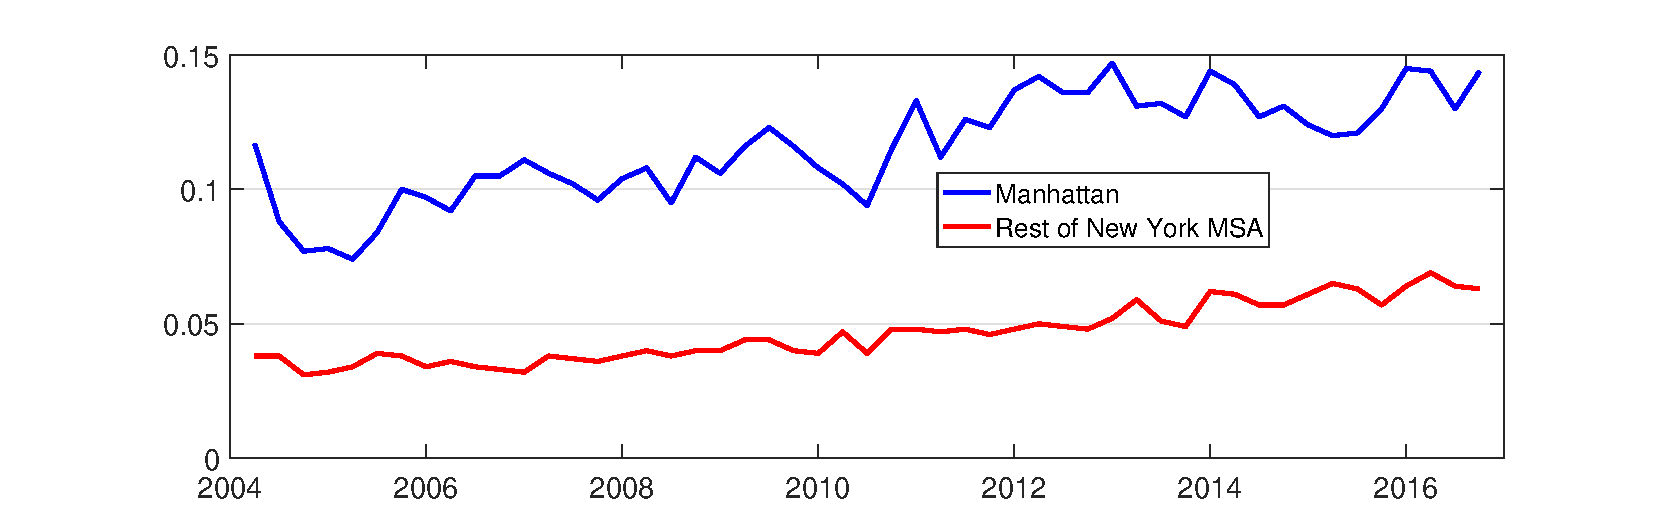
\includegraphics[width=5.5in,height=2.75in]{../Figures/OOTNY_v2}
\end{center}
\end{figure}

\citet{suher} provides corroborating evidence from New York tax records suggesting that, out of a sample of 84,000 condo units in the core of Manhattan in 2012, 25\% are owned by non-residents.\footnote{An April 2019 investigation by \emph{The Real Deal} corroborates these numbers. Out of 92,000 Manhattan condo units investigated, 16\% were bought by anonymous LLCs. One-third of units did not apply for the annual condo tax abatement available only to primary owners; those are pied-\'a-terre units. Stripping out units that are ineligible for the tax break raises the fraction of pieds-\'a-terre to 43\%.}

Evidence for the prevalence of vacant properties owned by non-residents comes from the American Community Survey data. It reports homes that are vacant for seasonal, recreational or other occasional use. Data for Manhattan show that the number of such vacant units has risen from 30.9\% of vacant units and 4.5\% of occupied units in 2010 to 39.3\% of vacant and 5.9\% of occupied units in 2015. This category of vacancies under-counts non-resident ownership because the category can only be assigned if no one responds to multiple contact requests by the surveyor. At that point, the surveyor will speak to neighbors, brokers, or property managers to try to figure out whether the unit is in fact occupied but only used occasionally. \citet{wheaton17} studies the ACS seasonal/occasional vacancy data and shows that they are related to regional variation in the amplitude of the house price boom and bust.

While non-resident buyers face no additional taxes to buy an apartment in NYC, despite public outcry for the introduction of such a tax, they face higher taxes than residents when selling. This includes Federal (20\%) and New York State (8.8\%) capital gains taxes as well as Federal estate taxes (no exemptions for foreigners). The Regional Plan Association backed a pied-\`a-terre tax for New York City in its 2018 Fourth Regional Plan, noting 60,000 NYC apartments are vacant but not on the housing market.

\paragraph{Rest of U.S.} The National Association of Realtors (NAR) has been conducting a  survey among its members on foreign home purchases in the United States since 2010. The share of foreign purchases was 10\% during the 12-month period that ended March 2017 (\$153bn). It was about 8\% in  the March 2015 (\$103.9bn), March 2016 (\$102.6bn), and the March 2018 (\$121bn)\ surveys. The 2018 foreign investment is approximately double the 2010 investment (\$65.9bn) when data collection started. Florida attracted most of the foreign investment in 2018 (22\%). Foreigners accounted for 50\% of purchases in Miami-Dade county. About 40\% of foreign purchases are by non-resident foreigners. OOT purchases would exclude  purchases by foreigners that are local residents but include all purchases by non-resident (out-of-MSA) U.S. citizens. Such data are not readily available for the entire U.S.

\citet{chincomayer:16} use housing transactions merged with tax assessor data to identify OOT buyers, using the property tax billing address. They find that the OOT share rises as high as 17\%\ in some boom markets like Las Vegas. \citet{bayerspec:11} use transaction data for the period 1988-2009 for Los Angeles county. They focus on the role of all investors, without distinguishing between local and out-of-town investors. Using three different measures, the investor share triples between the early 1990 to the peak of the boom in 2003-06.\footnote{Their measures of investors are (i) whether an individual owns two homes at the same time --this measure rises to a nearly 30\% share in 2006,-- (ii) purchases that were resold within two years --15\% of all homes bought in 2003-05 were resold within a two year period,-- and (iii) flippers defined as the fraction of purchasers who buy at least two houses while holding them for less than two years --this measure peaks at 5\% in 2006.}

\paragraph{London} A study by the Mayoral office shows that 13\% of properties sold in 2014-16 were bought by foreigners. Half of these homes were below \pounds 500,000, homes that could be bought by typical first-time home buyers. Separately, Knight Frank estimates that 49\% of Central London homes above \pounds1 million were sold to foreigners in the year to June 2013.
More than half of these sales (28\% of total sales) were to non-resident foreigners.

In April 2016, the U.K. began to levy a 3\%  stamp duty surcharge on second property purchases. Given the progressive schedule of stamp duty and the fact that OOT purchases are usually higher-end properties and always second homes, the incidence of this surcharge disproportionately falls on OOT buyers.


\paragraph{Paris} Data from \citet{CS:16} allow us to compute the share of OOT buyers in Paris. We define OOT buyers as either foreign or French residents who do not live in Paris or in Ile-de-France at the time of their housing purchase in Paris. These buyers account for 16.6\% of transactions (and a somewhat larger share of value) over the 1992-2016 sample. The OOT purchase share in Paris is fairly constant over time.

The Paris data also contain information on the use of the apartment, distinguishing between primary residence, investment property for rent, and secondary home (pied-\`a-terre). This information is available for all sales, and sellers can be grouped by residence at the time of sale. This data shows that 61\% of Parisian dwellings sold by OOT owners are secondary residences, with the remaining 39\% for rent.

\paragraph{Vancouver and Toronto} Foreigners owned 7.9\% of Vancouver's and 7.2\% of Toronto's condominium apartments   in mid-2017
according to Statistics Canada. Non-residents owned 5.1\% of all residential properties by value in Vancouver and 3.0\% in Toronto. Statistics Canada
suspects that these numbers understate foreign ownership because they fail to account for purchases made by corporations incorporated in Canada but controlled by foreign residents, as well as for properties bought by foreigners but in the name of a Canadian resident relative.\footnote{See https://vancouversun.com/news/local-news/foreign-ownership-data-released-so-far-just-the-tip-of-the-iceberg-statscan-director.}

Soaring prices prompted the government of British Columbia to introduce a 15\% transaction tax on foreign buyers in August 2016.
Foreigner buyers exclude foreign nationals who work and pay income taxes in British Columbia. This is consistent with the treatment of OOT buyers in our model: OOT investors do not work in the city either. The Government of Ontario  followed suit with its own 15\% transaction tax in April 2017. The levy in British Columbia was increased to 20\% in mid-2018, and now applies to a larger geographical area.
In the five weeks leading up  to the introduction of the tax, foreign buyers accounted for 10\% of purchase value
in the Vancouver metro area and 11\% in the City of Vancouver.

In April 2018, the City of Vancouver  instated an ``empty home tax" of 1\% of the taxable assessed value of the home for properties that are left vacant, i.e., that do not serve as primary residence or are not rented out at least six months per year. The province of British Columbia passed its own ``speculator" tax, which went into effect in 2019, targeting both foreign and domestic OOT home buyers who don't live in or rent out their properties for at least six months per year. The BC vacancy tax rate is 2\% of the home value for foreigners, 1\% for OOT residents, and 0.5\% for residents.

\paragraph{Australia and New Zealand}
Foreigners must apply with the government to purchase residential real estate in Australia. Data from Australia's Foreign Investment Review Board show a quadrupling of residential real estate approvals from 10,000 per year in the 2010-2012 period to 40,000 a year in 2015-2016. The 40,000 approvals correspond to \$72 billion in investment. The foreign buyer share hovered between 10 and 15\% between 2014.Q4 and 2017.Q1 according to the NAB. \

Approvals dropped to 13,000 in 2016-2017, totalling \$25 billion after the passage of stricter controls and higher application fees on foreign ownership.
The  province of New South Wales, where Sydney is located, introduced a stamp duty surcharge of 4\% on the purchase of residential real estate by foreign persons from June 2016 onwards. For purchases after July 2017, the surcharge was increased to 8\%. Victoria with capital Melbourne
introduced its own stamp duty surcharge of 3\% on July 1, 2015, and increased it to 7\% for purchases after July 1, 2016. Foreigners who live and work in Australia are exempt.
The  introduction of a ``ghost" tax on properties that are not available for rent or occupied more than half of the year and tighter Chinese capital controls may also have contributed to the decline in the foreign buyer share.
By 2017.Q4, it had fallen to 8.4\%.



 New Zealand similarly passed severe limitations on foreign home buyers in August 2018, after house prices surged. The non-resident share of home purchases peaked in April 2018 at 3.3\% in New Zealand, but at nearly 10\% in Queenstown and 7.3\% in Auckland.\

\paragraph{Singapore and Hong Kong}
The non-resident foreign purchase share in Singapore was 7.4\% in 2016.H1 and 6.8\% in 2017.H2. Singapore imposed a special tax of 15\% on foreign property buyers in 2013, and increased its tax to 20\% in August 2018.

Hong Kong introduced a 15\% non-resident stamp duty in 2012. Non-residents currently pay 30\% stamp duty in Hong Kong.

\paragraph{Israel} The share of residential properties owned by non-residents rose sharply from about 1\% prior to 2000 to 6\%\ in 2005-06 before falling back to 3\% by 2009, according to the Israeli Ministry of Finance. The share is much higher in Tel Aviv (about 8-10\%) and in Jerusalem (about 12-16\%). Starting January 2017, the purchase tax for non-residents was substantially increased, relative to that for residents.


\section{Model}

We model a housing market corresponding to a metropolitan statistical area (MSA). The MSA has a fixed population normalized to one.\footnote{Future work could consider an open-city model extension and study interactions between OOT investor flows and resident net migration patterns. Such a model would need to take a stance on a reservation utility of moving to other locations and on the moving costs. These would naturally differ by age, productivity, and wealth. A proliferation of parameters would ensue with little guidance from the literature on how to set these parameters. Evidence from the New York metropolitan area, discussed in Appendix \ref{app:dataNYC_migration}, suggests that net migration rates during the period of OOT inflows were small, and positively rather than negatively correlated with OOT purchase activity across time and space.} It consists of two geographies, the ``urban core" and the ``periphery." The urban core, which we refer to as zone 1, is the central business district  where all employment takes place. The periphery, or zone 2, contains the outer boroughs of the city as well as the suburban areas that belong to the metropolitan area.


\subsection{Households}

\paragraph{Preferences}
The economy consists of overlapping generations of households. There is a continuum of households of a given age. Each household maximizes utility $U$ over consumption goods $c$, housing $h$, and leisure $l$ (labor supply is $n$). Utility depends on location $\ell$, age $a$, and local public goods spending $G_t$:
\begin{eqnarray}
U(c_{t},h_{t},n_{t};\ell_{t},a,G_{t}) &=& \exp\left((1-\gamma) \theta G_t\right)  \frac{\left[\chi_{t}^{\ell,a} \mathcal{C}(c_{t},h_{t},l_t)\right]^{1-\gamma} }{1-\gamma} , \label{eq:prefs} \\
\mathcal{C}(c_t,h_t,l_t)&=&\left[(1-\alpha_n)\left((1-\alpha_h) c_t^{\epsilon} + \alpha_h h_t^{\epsilon}\right)^{\frac{\eta}{\epsilon}}+ \alpha_n l_t^{\eta}\right]^{\frac{1}{\eta}}   \label{eq:prefkernel}\\
 h_t &\geq& \underline{h} \label{eq:minhousesize} \\
n^a_t &=& \left\{\begin{array}{ll}1-\phi_{T}^\ell-\l_t \geq\underline{n}  & \text{  if  } a<65  \\
 0 & \text{  if  } a\geq65 \label{eq:minhours}
 \end{array}  \right. \\
\chi_{t}^{\ell,a}&=&\left\{\begin{array}{ll} \label{eq:shifter}
\chi^{1}  & \text{  if  } \ell=1 \text{ and  } a<65 \text{  and  } c_t<\underline{c}
\\ \chi^{1}\chi^W  & \text{  if  } \ell=1 \text{ and  } a<65 \text{  and  } c_t\geq\underline{c} \\
\chi^{1}\chi^R  & \text{  if  } \ell=1 \text{ and  } a\geq65 \\
1 &\text{  if  } \ell=2   \\
\end{array}  \right.
\end{eqnarray}
The coefficient of relative risk aversion is $\gamma$. The parameter $\theta \geq 0$ modulates the importance of the public good. The  function $\mathcal{C}$ is a CES aggregator of non-housing consumption $c$, housing consumption $h$, and leisure $l$. The Frisch elasticity of labor supply is affected by all utility parameters, but dominated by $\eta$. The parameter $\epsilon$ controls the intra-temporal elasticity of substitution between housing and non-housing consumption.

Housing is divisible and there are no moving costs. Equation \eqref{eq:minhousesize} imposes a minimum house size requirement ($\underline{h}$). Cities' building codes often contain such minimum size restrictions on dwellings.

Total non-sleeping time in equation \eqref{eq:minhours} is normalized to 1 and allocated to work ($n_t$), leisure ($l_t$), and commuting time $\phi_{T}^{\ell}$. We normalize commuting time for zone 1 residents to zero: $\phi_{T}^{2}>\phi_{T}^{1}=0$. Since we will match income data that exclude the unemployed, we impose a minimum constraint
on the number of hours worked ($\underline{n}$) for working-age households. This restriction will also help us match the correlation between income and wealth. There is an exogenous retirement age of 65; retirees supply no labor.

The age- and location-specific taste-shifter $\chi^{\ell,a}(c_t)$ is normalized to one for all zone 2 residents. The shifter $\chi^{1}$ captures the amenity value of zone 1 relative to zone 2. It captures relative school and air quality, crime, noise, and congestion, but also restaurants and cultural spaces. Whether $\chi^{1}$ is smaller or greater than 1 is an empirical matter. The parameter $\chi^W$ ($\chi^R$) shifts the utility for working-age (retired) households that live in zone 1 and consume above a threshold $\underline{c}$. Values for $\chi^W$ and $\chi^R$ above 1 capture a complementarity between living in zone 1 and high consumption levels, possibly reflecting luxury amenities located in the urban core. Such a luxury amenity effect provides an extra pull for rich households to live in the city center beyond the pull provided by the opportunity cost of commuting.  \citet{GHH:13}  achieve a similar outcome through a neighborhood consumption externality. %\comment{ A special case of the model arises for $\chi^{1}=\chi^R = \chi^W=1$; location choice is solely determined by commuting costs. Another special case is $\underline{c}=0$, which gives the same amenity value of the city center $\chi^{1}$ to all households, regardless of consumption level. We solve and discuss these special cases below.} \comment{\it{From Junjun: We don't have these cases in table 2 yet. Do you want me to add them?}}

There are two types of households in terms of the time discount factor. One group of households have a high degree of patience $\beta^H$ while the rest have a low degree of patience $\beta^L$. This preference heterogeneity helps the model match observed patterns of  wealth inequality and wealth accumulation over the life cycle. A special case of the model with $\beta^H=\beta^L$  is discussed below.

\paragraph{Endowments}
A household's labor income $y_t^{lab}$  depends on the number of hours worked $n$, the wage per hour worked $W$, a deterministic component $G(a)$ which captures the hump-shaped pattern in average labor income over the life-cycle, and an idiosyncratic, persistent, stochastic labor productivity state $z$. Idiosyncratic productivity risk is the main source of risk in the model, giving rise to market incompleteness.

There is an exogenous retirement age. After retirement, households earn a pension which is the product of an aggregate component $\overline{\Psi}$ and an idiosyncratic component $\psi^{z}$ which has a cross-sectional mean of one. The idiosyncratic component reflects productivity during the last period of the working stage. Labor income is taxed at rate $\tau^{SS}$ to finance the pension system.

Households face mortality risk which depends on age, $p^{a}$. Although there is no intentional bequest motive, agents who die leave accidental bequests. We assume that the number of people who die with positive wealth leave a bequest to the same number of agents alive of ages 21 to 65. The recipients are randomly chosen, with one restriction. Patient agents ($\beta^H$) only leave bequests to other patient agents and impatient agents ($\beta^L$) only leave bequests to other impatient agents. One interpretation is that attitudes towards saving are passed on from parents to children. Conditional on receiving a bequest, the size of the bequest $\widehat{b}_{t+1}$ is a draw from the relevant distribution (different for $\beta^H$ and $\beta^L$ types). Because housing wealth is part of the bequest and the house price depends on the aggregate state of the economy, the size of the bequest is stochastic. Agents know the distribution of bequests, conditional on $\beta$ type. This captures several stylized facts: many households receive no bequest, there is substantial heterogeneity among bequest sizes and ages at time of receipt for those who receive a bequest.%\footnote{As in \citet{Tabellini}, the young benefit from the unexpected house price appreciation of their owner parents through the type-specific bequest channel. Our bequest specification also captures that children have some idea about the kind of bequest they may expect to receive, and that bequests arrive at different points in the life cycle for different households.}


\paragraph{Location and Tenure Choice}
Let $S_{t}$ be the aggregate state of the world, which includes the wage $W_{t}$, the housing price $P^{\ell}_{t}$, the market rent $R^{\ell}_{t}$ and previous housing stock $H^{\ell}_{t-1}$ for each location $\ell$. The household's individual state variables are its net worth at the start of the period $x_t$, its idiosyncratic productivity level $z_t$, and its age $a$. We suppress the dependence on $\beta$-type in the problem formulation below, but note that there is one set of Bellman equations for each $\beta$-type. The household chooses each period in which location $\ell \in \{1,2\}$ to live and whether to be an owner or a renter. Denote by $V$ the value functions over these choices, with subscript $R$ denoting the choice of renting and $O$ that  of owning: \[V_{}=\max \left\{V_{O,1}, V_{R,1}, V_{O,2}, V_{R,2}\right\}.\]
The Bellman equations for $V_{R,\ell}$ and $V_{O,\ell}$ are defined below.


\paragraph{Renter Problem}
A renter household in location $\ell$ chooses non-durable consumption $c_{t}$, housing consumption $h_{t}$, and working hours $n_{t}$ to solve:
\begin{equation*}
\begin{array}{l}
V_{R,\ell}(x_{t},z_{t},a,S_{t})=\max\limits_{c_{t},h_{t},n_{t}}U(c_{t},h_{t},n_{t};\ell_{t},a,G_{t})+(1-p^{a})\beta E_{t}[V(x_{t+1},z_{t+1},a+1,S_{t+1})]\\ \text{   s.t.  }\\
c_{t} + R^{\ell}_{t} h_{t} + Q b_{t+1} + \phi^{\ell}_{F} = \left(1-\tau^{SS}\right)y^{lab}_t + \overline{\Psi}_t \psi^{z} + x_{t} \\
x_{t+1}=b_{t+1}+\widehat{b}_{t+1}\ge0\\
y_t^{lab} = W_{t}n_{t}G^{a}z_{t} \\
\text{  and equations } \eqref{eq:prefs}, \eqref{eq:minhousesize}, \eqref{eq:minhours}, \eqref{eq:shifter}.
\end{array}
\end{equation*}
In addition to a time cost, residents of zone 2 face a financial cost of commuting $\phi^{2}_{F}$. As we did for the time cost, we normalize the financial cost of commuting within zone 1: $\phi^{1}_{F}=0$.  The renter's savings in the risk-free bond, $Qb_{t+1}$, where $Q$ is the bond price, are obtained from the budget constraint. Next period's financial wealth consists of these savings plus any bequest received, $\widehat{b}$. Retirement income $\overline{\Psi}\psi^{z}$ is zero prior to age 65 and labor income is zero after age 65.

\paragraph{Owner's Problem}
An owner in location $\ell$ chooses non-durable consumption $c_{t}$, housing consumption $h_{t}$, working hours $n_{t}$, and investment property $\widehat{h}_{t}$ to solve:
\begin{equation*}
\begin{array}{l}
V_{O,\ell}(x_{t},z_{t},a,S_{t})=\max\limits_{c_{t},h_{t},\widehat{h}_{t},n_{t}}U(c_{t},h_{t},n_{t};\ell_{t},a,G_{t})+(1-p^{a})\beta E_{t}[V(x_{t+1},z_{t+1},a+1,S_{t+1})] \\\text{  s.t. }\\
c_{t}+P^{\ell}_t h_{t} + Q b_{t+1}+ P^{\ell}_{t}\widehat{h}_{t}+\phi^{\ell}_{F}
=\left(1-\tau^{SS}\right)y_t^{lab} + \overline{\Psi}_t\psi^{z}+x_{t} + R^{\ell}_{t}\widehat{h,}_{t}\\
x_{t+1}=b_{t+1}+\widehat{b}_{t+1}+P^{\ell}_{t+1}(h_{t}+\widehat{h}_{t})(1-\delta^{\ell}-\tau^{P,\ell}),\\ %-P^{\ell}_{t+1}\widehat{h}_{t}\delta_{inv}\\
-Q_{t}b_{t+1} \le  \kappa P^{\ell}_{t}(h_{t}+\widehat{h}_{t})-R_{t}\widehat{h}_{t} - ((1-\tau^{SS})y_t^{lab}-c_t)+\phi^{\ell}_{F,t},
 \\
\widehat{h}_{t} \ge 0,\\
\text{and equations } \eqref{eq:prefs}, \eqref{eq:minhousesize}, \eqref{eq:minhours}, \eqref{eq:shifter}.
\end{array}
\end{equation*}

Home owners in a zone are the landlords to the renters in that zone.\footnote{This assumption is not important for our results. The opposite extreme that all rentals are owned by non-locals would give rise to nearly identical quantitative results. The reason is that the equilibrium return on rental housing is close to the risk-free rate because risk aversion is low and the only source of aggregate risk, fluctuations in the OOT demand, displays only modest volatility.} For simplicity, we assume that renters cannot buy investment property and that owners can only buy investment property in the zone of their primary residence. Landlords earn rental income $R^{}_{t}\widehat{h}_{t}$ on their investment units $\widehat{h}_{t}$.

The physical rate of depreciation for  housing units is $\delta^{\ell}$. The term $Ph\delta^{\ell}$ is a financial cost, i.e., a maintenance cost.  As shown in equation (\ref{Eq:MarketClearingHousing}) below, physical depreciation is offset by residential investment undertaken by the construction sector.%\footnote{It is easy to solve for a model where investment housing incurs an additional maintenance cost which is a fraction $\delta_{inv} \geq 0$ of the value of the property. Increasing $\delta_{inv}$ makes renting less attractive and increases the home ownership rate, all else equal. We do not need a depreciation wedge to generate the observed home ownership rate.}
 Property taxes on the housing owned in period $t$ are paid in year $t+1$; the tax rate is $\tau^{P,\ell}$. Property tax revenue is used for local government spending  that enters the local residents' utility function.

Housing serves as a collateral asset for debt. For simplicity, mortgages are negative short-term safe assets.\footnote{It would be easy to introduce an exogenous mortgage spread. We could also add tax deductibility of mortgage interest rates. The implicit assumption here is that these two effects, one raising the mortgage rate and the other one lowering it, cancel out.} Households can borrow a fraction $\kappa$ of the market value of their primary residence and  investment property.\footnote{It is easy to introduce a different LTV limit for investment and primary housing.} Rental income and savings ($(1-\tau^{SS})y^{lab}-c$) in the first period (four years in the calibration) after the purchase of a rental property are excluded from household net worth when computing the LTV ratio.


\subsection{Firms}

\paragraph{Goods Producers} There are a large number $n_{f}$ of identical, competitive firms all of which produce the num\'eraire consumption good.\footnote{We assume that the number of firms is proportional to the number of households in the city when solving the model. With this assumption, our numerical solution is invariant to the number of households. Due to decreasing return to scale, the numerical solution would depend on the number of households otherwise.} This good is traded nationally; its price is unaffected by events in the city and normalized to $1$. The firms have decreasing returns to scale ($\rho<1$) and choose labor inputs to maximize profit each period:
\begin{equation}
\Pi_{c,t}=\max_{N_{c,t}} N_{c,t}^{\rho}-W_{t}N_{c,t}
\end{equation}

\paragraph{Developers} In each location $\ell$ there is a large number $n_{f}$ of identical, competitive construction firms (developers) which produce new housing units and sell them locally at a price $P^{\ell}_{t}$ per unit. All developers are headquartered in the urban core, regardless of where their construction activity takes place.
%\footnote{If some of the firms were owned locally, OOT demand would affect profits which would flow back to the locals. While our model misses this effect, there are two reasons why the effect is likely to be small. First, the capital share is only 1/3 of output. Our model captures 2/3 of the effect through labor payments. Second, while the construction profits go up, the consumption sector profits go down. The net effect is likely small, and would depend on what fraction of the firms in each sector are locally or nationally owned. Third, the empirical evidence suggests that the vast majority of developers operate in more than one metro area. For example, local developers only account for 12\% of apartment building transactions in the New York metro (RCA data).}
Let $H^{\ell}_{t-1}$ be the existing housing stock in zone $\ell$. The construction firms have decreasing returns to scale and choose labor to maximize profit each period:
\begin{equation}
\Pi_{h,t}^{\ell}=\max_{N_{h,t}^{\ell}}P_{t}^{\ell}\left(1-\frac{H_{t-1}^{\ell}}{\overline{H}^{\ell}}\right)\left(N_{h,t}^{\ell}\right)^{\rho}-W_{t}
N_{h,t}^{\ell} \label{eq:profith}
\end{equation}

The production function of housing has two nonlinearities. First, as for consumption goods firms, there are decreasing returns to scale because $\rho<1$. Second, construction is limited by zoning laws. The maximal amount of square footage zoned for residential use in zone $\ell$ is  $\overline{H}^{\ell}$. We interpret $\overline{H}^{\ell}$ as the total land area zoned for residential use multiplied by the floor area ratio (FAR), the maximum permitted number of floors that could be built on this land. This term captures the idea that, the more housing is already built in a zone, the more expensive it is to build additional housing. For example, additional construction may have to take the form of taller structures, buildings on less suitable terrain, or irregular infill lots. Therefore, producing twice as much housing requires more than twice as much labor. %Laxer zoning policy, modeled as a larger $\overline{H}^{\ell}$, makes development cheaper, and all else equal, will expand the supply of housing.

 When $\overline{H}^{\ell}$ is sufficiently high, the model's solution becomes independent of $\overline{H}^{\ell}$, and the housing supply elasticity is governed solely by $\rho$. When $\overline{H}^{\ell}$ is sufficiently low, the housing supply elasticity is lower and depends on both $\overline{H}^{\ell}$ and $\rho$.\footnote{In this sense, the model captures that construction firms must pay more for land when land is scarce. This scarcity is reflected in equilibrium house prices. In the background, the government makes available permits to build on land each period, in an amount normalized to 1 \citep{favilukis/ludvigson/nieuwerburgh:09}. }

%Because the depreciation rate of housing $\delta$ is positive, this production function implies that the total amount of housing is finite even if $\overline{H^{\ell}}=\infty$.
%The first order conditions imply that a firm in Zone $\ell$ has labor demand $N_{\ell,t}=\left(\frac{\left(1-\frac{H^{\ell}_{t-1}}{\overline{H^{\ell}}}\right)P^{\ell}_{t}\rho_{\ell}}{W_{t}}\right)^{\frac{1}{1-\rho_{\ell}}}$.

\paragraph{Profits}
Per capita profits from tradeable and construction sectors are: \[\Pi_t = \Pi_{c,t} + \Pi^{1}_{h,t} + \Pi^{2}_{h,t}\]
We assume that goods and construction firms are owned by  equity holders outside the city.   Below, we explore sensitivity to this assumption.


\subsection{Out-of-town Buyers}

OOT demand for housing is price elastic, stochastic, and persistent. OOT shocks are the only source of aggregate risk in the model. Shocks to the oil price,  to the exchange rate \citep{ruflevi}, political shocks in the country of origin \citep{BR:16} or in the destination country (e.g., Brexit) are all examples  of the underlying drivers of this stochastic OOT process. The persistence captures the notion that an OOT inflow is likely to last for a while, but could reverse in the future.\footnote{An alternative modeling approach would be to model the arrival of OOT buyers as an MIT shock. In that case, households would expect the OOT buyers to remain forever after. a MArkov process allows for the possibility of a reversal. With the benefit of hindsight, the data suggest at least a partial reversal in foreign purchases of U.S. real estate starting in 2018.} OOT buyers do not rent out their properties. Section \ref{sec:empevidence}, and in particular \citet{CS:16} provide empirical support for this assumption. Below, we  solve a version of the model that assumes OOT housing is rented out, with substantially different results. OOT buyers do not work in the local labor market, do not consume local public goods, and are not counted as part of city welfare.

Specifically,  OOT purchases  follow a two-state Markov process with a high state and a low state. In the low state, $OOT^{L}=0$ in both zones. In the high state, OOT purchases in zone $\ell$ are strictly positive and depend on the equilibrium house price with elasticity coefficient $b$:
\begin{equation}
\log\left(OOT_t^{H,\ell}\right) = a_{\ell} - b\log\left(P_t^{\ell}\right) \label{eq:OOT}
\end{equation}
Appendix \ref{app:OOTfoundation} provides two micro-foundations for this demand function based on either preference or wealth shocks to OOT investors. By virtue of the calibration, the model will match the observed price elasticity of housing demand by OOT investors.

We assume a symmetric transition probability matrix between the two OOT states, with one parameter $\pi$ governing the transition probability between regimes and therefore the expected duration of each regime.
Locals observe the aggregate OOT state, understand its law of motion, and consider it when making their optimal decisions.
%For realism, we restrict attention to the case where out-of-town buyers only acquire real estate in the city center (zone 1). The model can handle more general buying patterns.

\subsection{Equilibrium}

Given parameters and a stochastic process $\{OOT_t\}$, a competitive equilibrium is a price vector $(W_{t},P^{\ell}_{t},R^{\ell}_{t})$ and an allocation, namely aggregate residential demand by market renters $H^{R,\ell}_{t}$ and owners $H^{O,\ell}_{t}$, aggregate investment demand by owners $\widehat{H}^{\ell}_{t}$, aggregate housing supply, aggregate labor demand by goods and housing producing firms ($N_{c,t},N_{h,t}^{\ell}$), and aggregate labor supply $N_{t}$ such that households and firms optimize and markets clear.


The following conditions characterize the equilibrium. First, given wages and prices, firms optimize their labor demand, resulting in the first-order conditions:
\begin{equation}
N_{c,t}=\left(\frac{\rho_{}}{W_{t}}\right)^{\frac{1}{1-\rho_{c}}} \quad\text{and}\quad N_{h,t}=\left(\frac{\left(1-\frac{H_{t-1}^{\ell}}{\overline{H}^{\ell}}\right) P_{t}^{\ell} \rho }{W_{t}}\right)^{\frac{1}{1-\rho_{h}}}. \label{eq:foclabor}
\end{equation}Second, labor markets clear:
\begin{equation}
n_{f}\left(N_{c,t}+N^{1}_{h,t}+N^{2}_{h,t}\right)=N_{t}.
\end{equation}

Third, the housing market clears in each zone $\ell$:
\begin{equation}\label{Eq:MarketClearingHousing}
(1-\delta^{\ell})H^{\ell}_{t-1}+\underbrace{n_{f}\left(1-\frac{H^{\ell}_{t-1}}{\overline{H}^{\ell}}\right)\left(N^{\ell}_{h,t}\right)^{\rho}}_{INV}=H^{O,\ell}_{t}+\widehat{H}^{\ell}_{t}+OOT^{\ell}_{t}.
\end{equation}
The left-hand-side is the supply of housing which consists of the non-depreciated housing stock plus residential investment $INV$. The right-hand-side is the demand for those housing units by owner-occupiers, landlords, and out-of-towners.

% Housing market clearing in zone 2 is similar except for the OOT demand:
% \begin{equation}\label{Eq:MarketClearingHousing}
% (1-\delta^{2})H^2_{t-1}+\underbrace{n_{f}\left(1-\frac{H^{2}_{t-1}}{\overline{H}^2}\right)\left(N^2_{h,t}\right)^{\rho}}_{INV}=H^{O,2}_{t}+\widehat{H}^2_{t}.
% \end{equation}
Fourth, the rental market clears:
\begin{equation}
\widehat{H}^{\ell}_{t}=H^{R,\ell}_{t}
\end{equation}
Fifth, average pension payments equal to average labor income taxes collected:
\begin{equation}
\overline{\Psi}N_{ret}=\tau^{SS} E\left[N_{t}W_{t}\right],\label{eq:ss}
\end{equation}
where we used the fact that $G_a$ and $z$ average to 1 in the cross-section, and $N_{ret}$ is the total number of retirees, which is a constant.\footnote{For simplicity, we assume that the total pension payments are equal to the average of all social security tax revenues, where the expectation is across high and low OOT demand states. OOT demand affect wages and therefore the total social security tax collected in a city. We do not think that letting the pension fluctuate with OOT demand of local real estate would be desirable. In the U.S., Social Security is maintained at the national level, and pension payments do not depend on local-area variation in wages.}
Sixth, the aggregate state $S_{t}$ evolves according to rational expectations.
Seventh, the value of all bequests received is equal to the wealth of all agents who die. Eighth, local public goods spending equals property tax revenue. Appendix \ref{app:modeleq} presents first order conditions.

%\subsection{Numerical solution}

%If shocks to $z_{t}$ are permanent, then we can rewrite the household's problem such that $z_{t}$ is not a part of the state. In this case, the only individual state variable is the household's start of period wealth scaled by productivity $xs_{t}$. This will require a grid with around 40 individual gridpoints.

%If there are two zones, then the aggregate state $S_{t}$ consists of five prices $(W_{t}$,$R^{1}_{t}$,$R^{2}_{t}$,$P^{1}_{t}$,$P^{2}_{t})$ and two quantities $(H^{1}_{t-1},H^{2}_{t-1})$. If each is 4 gridpoints, this is a total of $4^7=16384$ gridpoints. Additionally, the quantity of housing demanded by foreigners will require a grid of size 2, for a total of 32768 aggregate gridpoints. Thus the total state space is 1310720 gridpoints.

%For owners, the choice set is zone (discrete choice of size 2), consumption, and residential investment. For renters the choice set zone and consumption.


%In the appendix we show that for renters, the choices of $h_{t}$ and $n_{t}$ are analytic functions of $c_{t}$, therefore the renter's problem can be rewritten with just two choices: consumption $c_{t}$ and location $\ell$. For owners, the choices of $h_{t}$ and $n_{t}$ are analytic functions of $c_{t}$ and $\widehat{h}_{t}$, therefore the owner's problem can be rewritten with just three choices: consumption $c_{t}$, investment property size $\widehat{h}_{t}$, and location $\ell$.


\subsection{Welfare effects on Locals from OOT Buyers}

We compute the welfare effect of an OOT inflow as follows. Suppose that OOT demand in period $t$ is low and that it stays low in period $t+1$. Denote agent $i$'s welfare at $t+1$ as $V_{t+1,i}(LL)$. Suppose instead that OOT demand at $t+1$ switches to high and denote agent $i$'s welfare in this situation as $V_{t+1,i}(LH)$. Agent $i's$ change in welfare from the OOT inflow in consumption equivalent units is (recall $\gamma$ denotes risk aversion):
\[\mathcal{W}_{t,i}=-1+\left(\frac{V_{t+1,i}(LH)}{V_{t+1,i}(LL)}\right)^{\frac{1}{(1-\gamma)(1-\alpha_{n})}}.\]
%Analogously, if foreign demand at $t$ is high, then agent $i$ would be willing to give up $\Delta^H_{t,i}$ in consumption equivalent units  to stay in the high state, where:
%\[ \Delta^H_{t,i}=-1+\left(\frac{V_{t+1,i}(HH)}{V_{t+1,i}(HL)}\right)^{\frac{1}{(1-\gamma)(1-\alpha_{n})}}.\]
It measures how much the household's value function, which reflects the entire expected present discounted value of future utility flows, changes upon a transition from the low to the high OOT state, expressed in consumption equivalent unit (in percentage points). It fully accounts for the persistent and stochastic nature of the OOT process. A positive number reflects a gain from the inflow, while a negative number reflects a loss. We compute aggregate welfare effects from ``inflows" by summing $\mathcal{W}_{t,i}$ across all agents, calling the resulting aggregate welfare measure $\mathcal{W}$.  We also sum separately among owners ($\mathcal{W}_o$) and renters ($\mathcal{W}_r$), for different age groups, income groups, and wealth groups. %Alternative summations by income or wealth are easy to do.
% We compute aggregate welfare effects from ``outflows" by summing $\Delta^H_{t,i}$.



\section{Calibration}

The baseline model is calibrated to the average U.S. metropolitan area. Appendix \ref{app:data} contains data sources and more detail.  Table \ref{Tbl:Calibration} summarizes the chosen model parameters. Externally calibrated parameters are indicated with a star.

\begin{sidewaystable}\caption{Calibration}\label{Tbl:Calibration}
\setlength{\tabcolsep}{4pt}
\renewcommand{\arraystretch}{1.05}
\begin{center}
{\scriptsize
\begin{tabular}{|l| c ll|}
\hline
Description                    & Parameter      & Values   & Target \\
\hline
 \multicolumn{4}{|l|}{Panel A: \textbf{Labor Income and Pension}}\\
\hline
Income states                  & $z$              & [{\IncStates}] &   Income distribution SCF  \\
Pension income*                & $\psi^{z}$       & [{\psiz}] &  Pension distr. rules     \\
Pension tax rate*              & $\tau^{SS}$      & {\taxss}  & Contribution rates\\
\hline
 \multicolumn{4}{|l|}{Panel B: \textbf{Preferences}}\\
\hline
Time Preference (4yr)               & $(\beta^L,\beta^H)$ & ({\PbetaL},{\PbetaH}) &  Wealth/income and wealth gini \\
Risk aversion*                      & $\gamma$            & {\Pgamma}      & Standard value      \\
Leisure weight*                     & $\alpha_{n}$    & {\alphaN}  & Average workweek    \\
Housing consumption weight*         & $\alpha_{h}$    & {\alphaH}  & Housing share in consumption of 21.6\%   \\
CES parameter consumption/housing*  & $\epsilon$      & {\ElastCH}   & Intra-temp elasticity c \& h of 2/3 \\
CES parameter consumption/leisure   & $\eta$          & {\ElastCN}     & Frish elasticity of labor supply of 1 \\
Minimum hours   & $\underline{n}$      & {\HoursMinbyHours} E[n]      & Capture part-time and full-time work  \\
Local Public Goods Preference   & $\theta$      & 1.15      &   \\
\hline
 \multicolumn{4}{|l|}{Panel C: \textbf{Finance and Regulatory}}\\
\hline
Bond Price (4yr)*               & $Q$            & {\PQ} & Avg return stock-bond portfolio 1987-2018   \\
Maximum residential/investment LTV*        & $\kappa$ & {\Pkappa} & Max LTV on primary residence/investment property    \\
Property tax (4yr)*             & $\tau^{P}$     & {\tauP}\%  & Property tax rates \\
Housing depreciation (4yr)*     & $\delta$   & {\deprH}  & BEA housing depr 1987-2018  \\
Minimum dwelling size* & $\underline{h}$ & {\HresMinbyHresRatio} $E[h]$  & Annual Housing Survey \\
\hline
 \multicolumn{4}{|l|}{Panel D: \textbf{Production and OOT Demand}}\\
\hline
Return to scale*  &$\rho_{c}=\rho_h^1=\rho_h^2$ & {\RTSC}  & Labor share of income   \\
%Return to scale construction   &$\rho_{h}$ & 0.5    & Housing supply elasticity of 1.0 (Saiz)   \\
Available space             & $(\overline{H}_1, \overline{H}_2)$  & ({\HBARone}, {\HBARtwo})  & Housing supply elasticity of 1.0  \\
Time-commuting cost*           &$\phi_{T}^{2}$       & {\PphiT}  & Avg. commuting time\\
Financial-commuting cost*      &$\phi_{F}^{2}$       & {\PphiF}   & Transportation spending BEA \\
OOT demand elasticity        & $b$ & {\OOTElas}   & Section 2 \\
OOT demand level         & $(a_1^{H},a_2^{H})$ & ({\OOTLevel})   & Section 2 \\
OOT demand transition prob.*   & $\pi$                   & {\Ppi} & Section 2    \\
Cons. externality threshold    & \underline{c} & {\Pchibar}    & Ratio of income zone 1/zone 2 avg. msa \\
Utility multiplier zone 1 all residents  & $\chi^1$   &{\PchiAll}    & Ratio of home ownership rate zone 1/zone 2 avg. msa\\
Utility multiplier zone 1 workers   & $\chi^W$       & {\PchiW}  & Ratio of rent zone 1/zone 2 avg. msa\\
Utility multiplier zone 1 retirees  & $\chi^R$       & {\PchiR} & Fraction of retirees in zone 1  \\
\hline
        \end{tabular}
}
\end{center}
\begin{minipage}{\textwidth}\tiny
    \smallskip{\it Notes:} The table reports the parameters of the model, their values in the baseline model and the the Vancouver model, as well as the target. Moments denoted with a * are externally calibrated. The other parameters are chosen to target a moment that is endogenous to the model.
    \end{minipage}
\end{sidewaystable}

\subsection{Demographics}
The model is calibrated so that one model period is equivalent to 4 years. Households enter the model at age 21, work until age 65, and retire with a pension after age 65. Survival probabilities $p(a)$ are calibrated to mortality data from the Census Bureau. People  age 65 and over comprise 18.3\% of the MSA population age 21 and over in the data and {\fracRet}\% in the model.\footnote{To speed up computation, we assume that the probability of dying is zero before age 36. The observed probability is below 1\% for each 4-year period before age 36. We use mortality tables from 1960 rather than the latest available ones so as to better match the observed share of agents above age 65 in the current population.}

\subsection{Labor Income}

Pre-tax labor earnings for agent $i$ of age $a<65$ is $y_t^{lab}= W_t n_t^i G^a z_t^i,$ where the household takes wages as given and chooses labor supply $n_t^i$. The choice of hours is subject to a minimum hours constraint, which is set to  {\HoursMinbyHours} times average hours worked.\footnote{This constraint rules out a choice of a positive but very small number of hours, which we do not see in the data given the indivisibility of jobs. It also rules out unemployment since the earnings data is for the (part-time and full-time) employed. The presence of the constraint enables the model to better match the observed correlation between wealth and income.} This constraint binds for {\HoursMinBind}\% of workers in equilibrium.


Efficiency units of labor $G^a z_t^i$ consist of a deterministic component that depends on age ($G^a$) and a stochastic component $z^i$ that captures idiosyncratic income risk. The $G^{a}$ function is chosen to enable the model to match the mean of labor earnings by age. We use data from ten waves of the Survey of Consumer Finance (SCF) from 1983-2010 to estimate $G^a$.

The idiosyncratic productivity process $z^i$ is chosen to match earnings inequality and to generate realistic persistence in individual earnings. We discretize productivity $z$ as a 3-state Markov chain. The values for the three states are chosen so that the average earnings of households in the bottom 25\%, middle 50\%, and top 25\% of the earnings distribution in the model matches those same objects in the 1983-2010 SCF. We assume a parsimonious transition probability matrix for $z$, where the probability of staying in the same productivity state is 90\% for the average worker and 100\% for retirees. The implied standard deviation and autocorrelation of the idiosyncratic component of labor income are 0.7 and 0.9, respectively, matching the micro evidence in \citet{StoreslettenTelmerYaron2006}. We refer the reader to appendix \ref{app:labinccalib} for details.

The Social Security tax rate, $\tau^{SS}$, is set to{\taxssper}\%. In the data, employees contribute 6\% and employers contribute an additional 6\%, but only on income below \$118,500. Retirement income is increasing in the household's last productivity level prior to retirement, but is capped for higher income levels.  We use actual Social Security rules to estimate each productivity group's pension relative to the average pension.  The resulting pension income states are $\psi^{z}= [{\Ppsizone},{\Ppsiztwo},{\Ppsizthree}]$, where $z$ reflects the last productivity level prior to retirement. Average budget balancing retirement income $\overline{\Psi}$ is \${\RetInc}, which corresponds to {\RetIncbyLabInc}\% of average earnings.



\subsection{Preferences}
The functional form for the utility function is given in equations \eqref{eq:prefs} and \eqref{eq:prefkernel}. We set risk aversion $\gamma={\Pgamma}$, a standard value in the macro-finance literature.

We set $\alpha_{n}$ to match the average workweek of 34.5 hours per week in the U.S., which is 30.8\% of non-sleeping time (112 hours per week).
The model generates {\AvgHours} \%.

We set $\alpha_{h}$ to match the ratio of housing consumption to total consumption. The average in U.S. data for 1987-2018 (BEA real housing services consumption to real non-durable plus real services consumption) is 22.1\%; the model generates {\HousTotConsratio}\%.

The parameter $\epsilon$ governs the intra-temporal marginal rate of substitution between housing and non-housing consumption. While the literature contains a range of estimates, the median elasticity across studies is 2/3, resulting in $\epsilon=-0.5$. We provide sensitivity analysis below.

The parameter $\eta$ governs the Frisch elasticity of labor supply, alongside the other utility parameters. Here too, there is a wide range of estimates from 0 to 1.5 based on micro data and from 2 to 4 based on macro data. We target a value of 1, resulting in $\eta = 0$. We obtain a Frisch elasticity in the model of {\FrischEMacro} using aggregate quantities and {\FrischEMicro} when using individual quantities.

We set $\beta^H={\PbetaH}$ ({\PbetaHy} per year) and $\beta^L={\PbetaL}$ ({\PbetaLy} per year).\footnote{ Note that because of the probability of death, the effective time discount rate is $(1-p(a))\beta$, which is less than one.} A 25\% share of agents has $\beta^H$, the rest has $\beta^L$. This delivers an average $\beta$ of {\Pbeta}, chosen to match the average wealth-income ratio which is 5.69 in the 1998-2010 SCF data. The model generates {\NWbyInc}. The dispersion in betas delivers a wealth Gini coefficient of {\GiniNW}, close to the observed wealth Gini coefficient of 0.80 for the U.S.

The probability of receiving a bequest equals the number of dead households divided by the number of households between ages 21 and 65. It is equal to {\Probbequest}\% over each 4-year period, and identical for $\beta^H$ and $\beta^L$ household types. Under our calibration, {\fracbeqann}\% of wealth is bequeathed each year, close to the 1.2\% in the data.

%The parameter $\theta \geq 0$ modulates the importance of the public good in the utility function. It captures the government's efficacy at converting a given amount of tax revenue into valuable public goods. The public finance literature provides little guidance on how to set $\theta$. Values of $\theta$ below 1 imply that the average household is unwilling to forgo private consumption for more public goods. Values of $\theta$ above 2 imply that households want to forgo so much private consumption that optimal government tax revenue would end up above  50\% of private consumption. In our baseline calibration, we set $\theta=1.15$. It implies that the property tax rate we set generates  property tax revenue which is \comment{5\%} of private consumption. This is close to the observed  share of local tax revenue in local GDP.\comment{Tighten up and look at the data here.}
The parameter $\theta\geq 0$ modulates the importance of the public good in the utility function. It captures the government's efficacy at converting a given amount of tax revenue into valuable public goods. When $\theta=0$, government spending is wasteful. Values of $\theta$ below 1 imply that the average household is unwilling to forgo private consumption for more public goods. Values of $\theta$ above 2 imply that households want to forgo so much private consumption that optimal government tax revenue would exceed 50\% of private consumption. The public finance literature provides little guidance on how to set $\theta$. We set $\theta = 1.15$  in our benchmark model and provide sensitivity analysis.
%In the benchmark model, the property tax rate of 6.3\% (per 4 years) raises government revenue equal to {\TaxbyInc}\% of personal income. In the U.S., property taxes account for 1.8\% of personal income.\footnote{This is based on Census data compiled by the Urban Institute-Brookings Institution Tax Policy Center. Their Table 51 reports state and local general revenue by source for 1977-2015. This allows us to compute property tax revenue as a share of total state and local government revenue. Their Table 71 reports state and local tax revenue as a share of personal income, every five years from 1977 until 2002 and annually from 2004 until 2015. Combining the two results in a time series for property tax revenue relative to personal income. The series is nearly constant over time at around 1.8\%.} Thus the property tax rate is higher than would optimally be chosen by a benevolent social planner.

The taste-shifter for zone 1 is parameterized as: $\chi^{1}={\PchiAll}$,  $\chi^{W}={\PchiW}$, $\chi^{R}={\PchiR}$, $\underline{c}={\Pchibar}$.  We chose these four parameters to get our model to better match the following four ratios of zone 1 relative to zone 2 variables, given all other parameters: the relative fraction of retirees of 0.84, a relative household income ratio of 1.12, the relative ratio of market rents per unit of 1.03, and the relative home ownership rate of 0.65. In the model, these ratios are {\fracRetRel}, {\IncRel}, {\MedMktRentbySqftRel}, and {\HORel}, respectively. The parameters imply that the amenities of zone 1 are 7\% below those of zone 2 for households who consume below the threshold. The financial commuting cost compels these lower-income households to live in zone 1. Matching the relative income and rent ratios requires net disamenities for the city center. About {\cbarFrac}\% of the agents in the model consume above the threshold  $\underline{c}$. They like zone 1 better than poorer agents, especially the retirees ($\chi^1\chi^R={\PchiAllchiR}$).


\subsection{Production and Housing }
The return to scale parameter in the both sectors is set to $\rho={\RTSC}$ to match the observed labor share of output of 66\%.

The two zones in the MSA differ in the maximum buildable residential square footage permitted by existing zoning rules, $\overline{H}^{1}$ and $\overline{H}^{2}$. We use two moments to pin down the two parameters. The first moment is the fraction of households in the metro area that lives in the urban core. In 2017 data for the largest 74 U.S. MSAs, that fraction is 22.8\%. The second moment is the long-run housing supply elasticity in the metro area. \citet{Saiz:10} estimates housing supply elasticities for the largest 50 MSAs; they range from 0.6 for Miami to 1.70 for Albany. We target  a value of 1.0, the weighted average of the housing supply elasticities, weighted by the MSA population shares. The model generates a supply elasticity of {\HSE}; Appendix \ref{app:HSE} contains the derivation. The housing supply elasticity is much lower in zone 1 ({\HSEone}) than in zone 2 ({\HSEtwo}), because in zone 1 the housing stock is much closer to $\overline{H}^{1}$ ({\HbaroneDist}\% from the constraint) than it is in zone 2 ({\HbartwoDist}\% from the constraint). Since the housing stock of the metro area is concentrated in zone 2, the city-wide elasticity is dominated by that in zone 2.\footnote{In recent work, \citet{BaumHan2020} find slightly lower average housing supply elasticities of 0.6-0.7 at the MSA level as \citet{Saiz:10}. Looking at more disaggregate data, they also find that housing supply elasticities are substantially lower in the urban core than in the periphery.}

We set the maximum loan-to-value ratio (LTV) on mortgage debt at 90\% ($\kappa=\Pkappa$), implying a 10\% down payment requirement. The observed mean combined LTV ratio at origination for U.S. mortgages in the U.S. is 87.3\% as of October 2016 according to the Urban Institute and has consistently been above 80\% since the start of the data in 2001. %The LTV for investment property is set at 80\% ($\theta_{inv}=0.8$), consistent with higher downpayment requirements for investment properties.

We set the property tax rate $\tau^{P}={\tauP}\%$ or {\tauPy}\% per year. This is the population-weighted average property tax rate among the 74 largest MSAs in 2016, using data from the American Community Survey and the Zillow Home Value Index. Separate calculations for property tax rates in zones 1 and 2 of these MSAs show nearly identical averages. %The revenue from this tax is used to fund local public goods. In the baseline model, local residents derive no utility from public goods. We relax this assumption in Section \ref{sec:Vancouver}.

We assume that property depreciates at 2.45\% per year and set $\delta={\deprH}$. This is the average depreciation rate for privately-held residential property in the BEA Fixed Asset tables for the period 1987-2016. %It is also consistent with the 27.5 year life span over which the IRS allows for the depreciation of rental property.


The price for the one-period (4-year) bond is set to $Q={\PQ}$ to match the population-weighted average house price-to-rent ratio in the largest 74 MSAs using Zillow data. This ratio is 13.03. The model delivers {\MedMktPHbyMedMktRent}. The implicit interest rate is {\ImInt}\% per year.\footnote{Households in the model only have access to a real bond to save in (beside housing). In reality, a wider range of investment opportunities is available and governs wealth accumulation in the data. The average real return on a 50-50 bond-stock portfolio over the period 1987-2018 is 5.05\%, where the bond is the five-year constant maturity Treasury and the stock is the CRSP value-weighted stock index.}

Finally, we impose a minimum housing size of {\HresMin} square feet, or {\HresMinbyHres}\% of the average housing unit size.  According to the American Housing Survey, the average housing unit (including single- and multi-family units) built after 1960 is about 1,600 square feet  big.

\subsection{Commuting Costs}

We set the time cost of commuting to the observed commuting time in the largest 74 MSAs. The average one-way commuting time to work in the data is 28.6 minutes according to the 2017 American Community Survey of the U.S. Census. This data number is a weighted average of commutes within zone 1 and from zone 2 to zone 1. Since the model normalizes the commuting time within zone 1 to zero, we target the additional commuting time of zone 2 residents of 24.2 minutes per trip for 10 commuting trips per week.\footnote{Given that 22.8\% of the population lives in zone 1 as in the data (and matched by the model), and assuming a 10 minute commute within zone 1, the metro-wide average commute of 28.6 minutes implies an average commute from zone 2 to zone 1 of 34.2 minutes, or 24.2 minutes longer than the commute within zone 1. Under this assumption, commutes within zone 1 represent 8\% of total commuting time.} The 4.0 hours represent {\CommCost}\% of the 112 hours of weekly non-sleeping time. Hence, we set $\phi_{T}^{2}={\PphiT}$.

The financial cost of commuting $\phi_{F}^{2}$ is set to {\CommCostFinbyInc}\% of average labor earnings, or  \${\CommCostFinDollar} per household per year. This is a reasonable estimate for the commuting cost in excess of the commuting cost within zone 1, which is normalized to zero.\footnote{Aggregate spending on transportation services accounts for 3.9\% of aggregate non-durable and services consumption and the same fraction of compensation of employees. We choose a slightly lower number given that only zone 2 residents commute. A 2015 survey by Citi, the Citi ThankYou Premier Commuter Index, finds that the average commuter spends \$2,600 per year on their commute, which is close to our chosen value.}


%We set the \emph{financial} cost of commuting for workers such that the model generates transportation expenses that are 3.8\% of total consumption. This is the average value in the U.S. data for 1987-2018 (BEA real transportation spending to real non-durable plus real services consumption). Some of these transportation costs are incurred by zone 1 residents. If we assume that zone 1 residents spend 1/4 as much on transportation expenses than zone 2 residents, then $\phi_{F}^{1}=0.0115$ and $\phi_{F}^{2}=.0460$ match the nationwide average of 3.8\% given the population shares.

%We assume that retirees have time and financial commuting costs that are $1/3$ of those of workers. This captures that retirees make fewer trips, travel at off-peak hours, and receive large discounts for transportation.

\subsection{OOT share}

We set the low OOT state to reflect a situation without (before) OOT real estate purchases: $OOT^L=0$. Given the empirical evidence discussed in Section 2 for several of the world's major MSAs, we target a 10\% share of housing demand by OOT buyers in the city center and a 5\% share in zone 2. We set the parameter $a_{\ell}$ in equation \eqref{eq:OOT} to obtain the target share, given the value for $b$.

For  the price elasticity of demand coefficient $b$, we consider two values. First, \citet{suher} estimates a  price elasticity of 0.6 using a 2013 experiment in New York City when a property tax abatement was phased out for non-residents only. We use this 0.6  estimate as our benchmark value for $b$. The second value comes from matching the observed change in OOT home purchases in Vancouver in response to the introduction of the OOT transaction tax in August 2016. The 15\% transaction tax raised prices for OOT buyers by 15\%. The share of OOT purchases in Vancouver in the five weeks prior to the OOT tax was  10\%.\footnote{Official statistics indicate a 10\% share for the period from June 10 until July 16, 2016. This period excludes the two weeks prior to the announcement of the tax and another month prior to the introduction of the tax, during which anticipation buying may have artificially inflated the foreign purchase share.  Several articles indicate that a foreign purchase share of 10-13\% was common for metro Vancouver in the months before June 10, 2016. E.g., \url{http://www.rew.ca/news/foreign-purchases-of-vancouver-homes-rise-slightly-as-market-adjusts-to-tax-1.3412049}. } After the tax was introduced the OOT share fell to 4.1\% of purchases.\footnote{The 4.1\% share is for January 2017. Because of the initial bunching of OOT purchases prior to August 2016, there was a sharp drop-off in the immediate aftermath of the introduction of the tax. The foreign share was only 1.8\% in September 2016 and gradually started to increase to 3-4\% in the October 2016-January 2017 period. Foreign purchases fell from 4.1\%\ to 2.5\% by mid-2017 before  rising again to 4.9\% in early 2019. The post-January 2017 changes are likely due to reasons other than the transaction tax.\ } The implied price elasticity is $(\log(0.041)-\log(0.10))/(\log(1.15)-\log(1))=6.4$. This much higher sensitivity may reflect substitution of foreign purchases to other Canadian or U.S. cities (e.g., Toronto and Seattle) in response to the Vancouver tax increase. We use this second value for an important sensitivity check.

We assume a state transition probability between the low and the high OOT regimes of 10\% per 4-year period. That is, $\pi=0.90$. Given the uncertainty regarding these numbers, we explore changing  $a$, $b$, and $\pi$ below.






%\paragraph{City-center Amenities}

%If a household lives in zone 1 and consumption is higher than $\underline{c}$, then the taste shifter takes on the value $\chi^W>1$ for workers and $\chi^R$ for retirees. This amenity effect creates a complementarity between living in zone 1 and high consumption levels. This modeling device stands in for a certain luxury consumption good bundle (high-end entertainment and restaurants) that is only available in the urban core. This modeling device is similar to the neighborhood consumption externalities modeled in \citet*{GHH:13}.

%We choose $\chi^{W}=1.05$, $\chi^{R}=1.086$, $\underline{c}=0.70$. The latter number implies that 11\% of the population is above the consumption cutoff. We target the 1.12 ratio of zone 1 to zone 2 per capita income in the average MSA, the 1.03 ratio of rents in zone 1 to zone 2 in the average MSA, and the 0.9 fraction of retirees in zone 1 to zone 2.


\section{Baseline Model Results}

%We are reluctant to further increase risk-free interest, depreciation or tax rates to lower the price-rent ratio in the model, since we have chosen high values for these parameters already.
This section discusses the baseline results. In the next section, we switch off several features of the model one by one, to explain and quantify the role of the various model ingredients.

\subsection{Earnings, Wealth, and Home Ownership}


A first check on the model concerns its ability to broadly match observed patterns in  income, wealth accumulation and home ownership over the life cycle.

The top panels of Figure \ref{Fig:WealthByAgeBaseline} show pre-tax earnings by age in the data (left panel) and in the model (right panel). The solid black line shows the well-known hump-shaped labor income profile over the life cycle for the median household. The dashed red line shows average labor income in the bottom 25 percent of the labor income distribution, the dash-dotted blue line reports average income among the middle 50 percent of the income distribution, and the dotted green line shows the average income among the top-25\% of the distribution. The model matches the observed labor income profiles closely. Since hours worked are a choice variable, the good fit of labor earnings means that model has realistic implications for hours worked. Our assumption of a constant income in retirement after age 65 causes a more discrete decline in income than in the data, presumably because some people continue to work after age 65 in the data.


\begin{figure}\caption{Earnings, Net Worth, and Home Ownership across Age and Income groups} \label{Fig:WealthByAgeBaseline}
\begin{center}
\includegraphics[width=7in,height=8in,trim=1cm 0.5cm 1cm 0.5cm]{../Figures/city_fig_wealth_data_model_updated}
%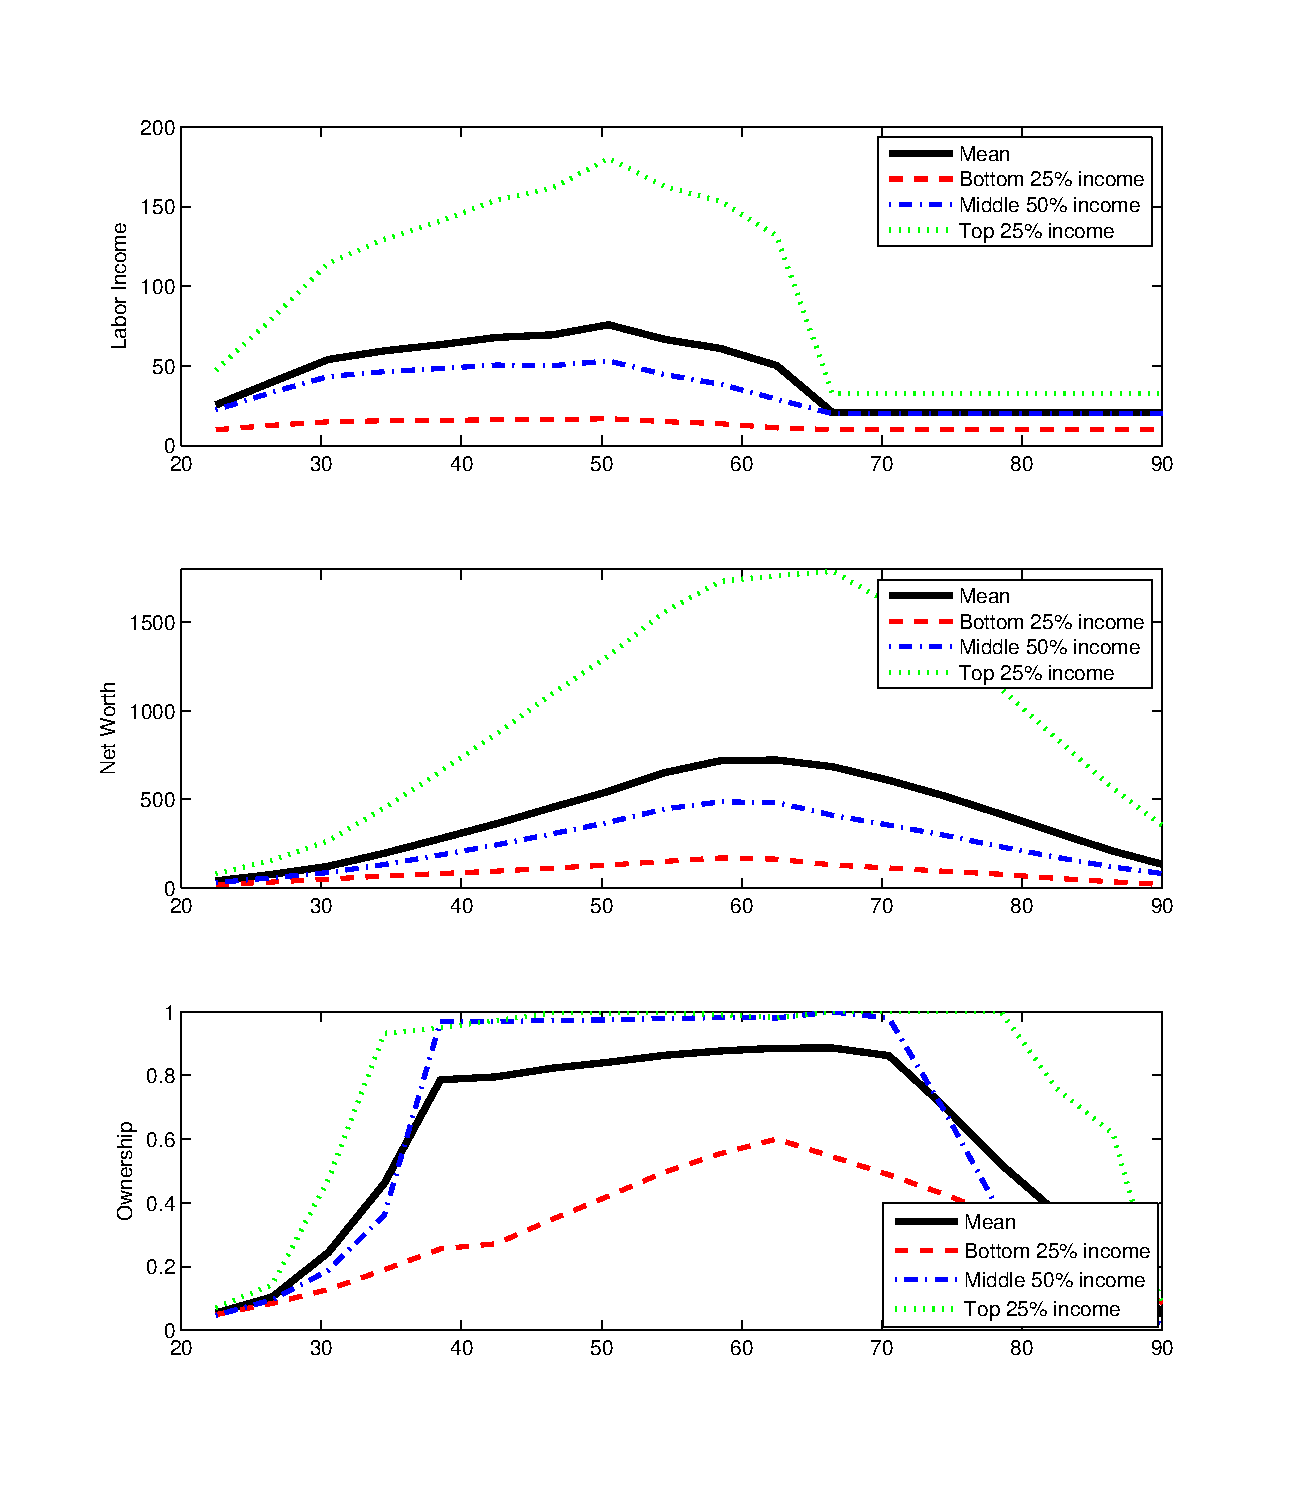
\includegraphics[width=3.2in,height=8in,trim=1cm 0.5cm 1cm 0.5cm]{../Figures/city_fig_wealth_baseline}
\end{center}
\vspace{-1cm}
\begin{minipage}{\textwidth}\tiny
    \smallskip{\it Notes:} The left panels are for the data and based on the Survey of Consumer Finance (all 1983-2010 waves). All survey data are first expressed in 2010 real dollars before averaging across survey waves. The right panels are for the benchmark model. The top row denotes household earnings. The middle row denotes household wealth. The bottom row denotes the home ownership rate.
    \end{minipage}
\end{figure}


Wealth and home ownership result from households' optimal consumption and investment decisions. The middle panels of Figure \ref{Fig:WealthByAgeBaseline} plot household net worth, defined as real estate wealth plus financial wealth minus debt. The bottom panels plot the home ownership rate.

The model generates a home ownership rate of {\AvgOwnRate}\% ({\AvgOwnRateB}\% prior to the OOT inflow), close  to the observed home ownership rate of 60.6\% for the average U.S. MSA in 2016.
The model fits the life-cycle patterns of  wealth accumulation and home ownership well. The average home ownership rate starts out below 20\% for the youngest households and displays a hump-shaped pattern over the life-cycle. It peaks at about 80\% around age 70 in both model and data. It then declines in retirement. Home ownership rates were not targeted in the calibration, so this is an important success for the model.

The model also generates about the right amount of average wealth at different ages during the working stage of life. Households accumulate about \$250,000 by age 40 and \$650,000 by age 65, on average, in both model and data. Wealth gradually declines in retirement, in large part because home ownership rate declines. Both the decline in home ownership and total wealth are steeper in the model than in the data, and closely connected to each other.\footnote{Allowing for an intentional bequest motive and/or adding late-in-life medical/long-term care risk would give households additional motives to slow down wealth decumulation \citep{ACLVN:11}. So would giving elderly people a preference for ``aging in place" or letting them forgo housing maintenance \citep{CoccoLopes:17}. Adding these motives would overly complicate the model whose main purpose is to analyze the effect of OOT investors.}


The model generates substantial cross-sectional variation in wealth and home ownership across cohorts and income groups that is broadly consistent with the data. The model matches the  Gini coefficient for wealth ({\GiniNW} in model and 0.78 in data), which substantially exceeds the Gini of income ({\GiniInc} in model and 0.46 in data). %The average wealth held by the top-25\% of income earners is somewhat higher than in the data while the share of wealth held by this group is somewhat lower (61\% in the data and 48\% in the model).



\subsection{House Prices and Rents}

House prices, rents, and wages are determined in equilibrium. Since risk premia are small, as can be expected from a model with CRRA preferences and risk aversion of 5, the house price-to-rent ratio is close to the one arising from the user cost formula:$(1-Q\times(1-\delta-\tau^{P}))^{-1}=3.28$ or 13.1 annualized. This 13.1 ratio in the model is close to the 13.0 average across the 75 largest MSAs in the U.S. data. The model also matches the relative ratio of rents between zones by virtue of the calibration. The quantity and price results suggest that the model is well positioned to quantitatively evaluate both the average and the distributional consequences of OOT purchases.

\subsection{Main Results: Increase in OOT Purchases}
%In the baseline model, the average OOT demand in Zone 1 (Zone 2) takes on two values, 10\% (5\%) of housing in the high state and 0 in the low state. OOT fluctuations are the only source of aggregate risk in the economy. Conditional on a switch, each regime is expected to last 40 years. %Because of the high persistence of the OOT demand process, the model with stochastic OOT demand that is in the low (zero) OOT demand state produces moments that are similar to the model without any OOT demand.

Table \ref{Tbl:MomentsPrice} summarizes how key prices and quantities adjust in response to the OOT shock.  The first row  reports the short-run response,  in the first (four-year) period after the economy switches from the low to the high OOT state. These short-run changes are denoted by $\Delta_1$  and expressed as percentage changes. The second row reports long-run changes, denoted by $\Delta_{ss}$, measured as the difference between the high-OOT and low-OOT stochastic steady states.  The last three columns report welfare effects for the average renter, for the average home owner, and average across all households.

\paragraph{Short-run response}
The increase in OOT demand for housing is partly met by new construction. In zone 1, where the OOT inflow is 10\%, residential investment increases by {\BaselineINVone{2}{0}}\% in the short-run. Additional construction accommodates 16\% of the OOT housing demand. The low housing supply elasticity (due to stricter zoning) is responsible for the less than one-for-one supply response. To clear housing markets, locals must therefore consume less housing. To induce a sufficiently large decline in local housing demand, rents rise by {\BaselineRone{2}{0}}\% in zone 1. House prices rise by {\BaselinePone{2}{0}}\%. Thus, the arrival of OOT investors leads to a significant increase in the cost of housing in the first four years. It not only increases the prices of owner-occupied housing, which the OOT investors buy, but it has an even larger effects on rents. Rental and owner-occupied units are part of the same market for space.

Because OOT demand  is mean-reverting, an OOT inflow today implies lower expected future OOT demand and hence rental growth. Prices go up by less than rents since they capitalize the expected lower rent growth; the price-rent ratio declines ({\BaselinePoneByRone{2}{0}}\%).\footnote{The risk premium associated with OOT demand fluctuations is small, and does not fluctuate much with the OOT state. Discount rate variation explains little of the price-rent dynamics. To generate meaningful variation in housing risk premia would require additional sources of aggregate risk such as changes in mortgage lending standards as in \citet{favilukis/ludvigson/nieuwerburgh:09}.}

In zone 2, where the OOT inflow is 5\%, residential investment increases by {\BaselineINVtwo{2}{0}}\% in the short-run. The larger expansion in the housing stock in zone 2, despite the smaller OOT inflow, is due to the larger housing supply elasticity in zone 2 which itself reflects the larger availability of undeveloped space $\overline{H}^2$. Zone-2 rents rise by {\BaselineRtwo{2}{0}}\% and prices rise by {\BaselinePtwo{2}{0}}\%, nearly as much as in zone 1 despite the smaller relative OOT demand and the larger supply response. In the MSA's spatial equilibrium, changes in rents and prices in zone 2 cannot differ by too much from changes in zone 1, lest they trigger large migration from zone 1 to zone 2. Commuting costs and amenity differences segment the housing markets of the two zones but spatial equilibrium forces bind them together.


The model's predicted response of house prices to an increase in OOT buyers is similar to that estimated in recent empirical work. Using a difference-in-differences design, \cite{GorbackKeys2020} estimate that U.S. zip codes with a high foreign-born population share experienced a 3.2\% larger increases in foreign demand, price increases of around 5\%, and housing stock increases of around 1.6\% relative to zip codes with low foreign-born shares.\footnote{The instrumented increase in foreign purchases understates total OOT purchases because (i) it excludes domestic OOT buyers, (ii) the foreign purchase surge lasted longer than 4 years, (iii) their DiD estimates do not include non-Chinese foreign-born residents, and (iv) the DiD estimates cannot capture any aggregate trend affecting all zip codes at the same time.} These numbers are broadly consistent with our baseline model where OOT purchases of 6\% (10\% in zone 1 and 5\% in zone 2) of the housing stock lead to short term (4-8 years) price increases of 6.4\% and supply increases of 1\%. The price increase is smaller and the supply increase is bigger in the long run.

\paragraph{Composition effect}
An interesting population composition effect takes place in response to the OOT inflow which helps explain the rent and price effects. High-wealth, middle-aged households leave zone 1 for zone 2; they sell to the OOT buyers. The average wealth and income of zone-1 residents in the 44-64 age group falls by {\NWMidChZoneOne}\% and {\WageMidChZoneOne}\%, respectively. The home ownership rate among locals in zone 1 falls by{\OwnLocalChangeZoneOne}\% since many in this demographic are owners. The increase in house prices brought about by the OOT inflow makes living in a large zone-1 home expensive for this group. The higher prices also make it harder to satisfy the housing collateral constraint for households that are not already owners in zone 1. By the same token, this group now demands a lot of housing in zone 2 where house prices are much lower per square foot. The increase in demand for zone-2 housing by this group helps explain the large rent and price increases in zone 2. It also explains the increase in home ownership among locals in zone 2 (+{\OwnLocalChangeZoneTwo}\%).

In contrast, after the OOT inflow, the young (and thus low-wealth), high-income group becomes more prominent in zone 1. Due to its high productivity, this group has a high opportunity cost of commuting and a high marginal value for zone-1 housing. They tend to live in smaller housing units. This reverse population flow of the young high-productivity households helps explain why the zone-1 local population only falls modestly ({\BaselineZoneOneFrac{2}{0}}\%). The OOT inflow crystalizes who among the locals has the highest value of space.

\paragraph{Housing affordability}
The price-income ratio in the model, denoted $HP/Y$ in the table, is computed as the average house price per square foot, $P$, multiplied by the average house size in square feet divided by the average earnings of working-age households $Y$. Because we want to compare the same house across OOT states, we hold the average house size in a zone fixed at its unconditional average.
The price-income ratio in zone 1 (zone 2) increases  by {\BaselineHPoneByY{2}{0}}\% ({\BaselineHPtwoByY{2}{0}}\%). These changes are much larger (smaller) than house price changes in zone 1 (zone 2) since some higher-income households move from zone 1 to zone 2 in response to the outflow, lowering (increasing) average income in zone 1 (zone 2).
A second major housing affordability indicator is the fraction of income spent on rent, denoted $HR/Y$. Average rent is the rent per square foot $R$ multiplied by the average house size; it is divided by average working-age earnings. The rent-income ratio rises by {\BaselineHRoneByY{2}{0}}\% in zone 1 ({\BaselineHRtwoByY{2}{0}}\% in zone 2). By these common metrics, OOT buyers reduce housing affordability substantially. They do so disproportionably in the city center.

\paragraph{Labor Market}
OOT demand drives up wages by {\BaselineW{2}{0}}\%. The share of construction employment increases by {\FracConstructChShort}\% (construction share of hours worked rises from{\FracConstructBefore}\% to{\FracConstructAfter}\%) as additional housing is built upon the OOT inflow. The construction employment share then slowly falls, but remains at a higher level as long as OOT demand remains high because the higher housing stock requires more maintenance. To reallocate workers from the non-housing to the housing sector, equilibrium wages must rise. Higher city-wide wages lead to lower aggregate labor demand, with hours worked falling{\HoursWorkedChange}\%.   In sum, the OOT influx prompts an increase in wages and a boom in the non-tradable sector, but also to a loss in competitiveness and a fall in employment in the tradable sector.\footnote{Although housing is the only non-tradable good in our model, the same intuition carries over to any other non-tradable goods and services that OOT consume when they are in town, e.g., restaurants or entertainment.} The increase in wages is offset by a reduction in hours worked, leaving average earnings down by \EarningsChange\%. Cost of housing increases translate (slightly more than) one-for-one into cost of living increases.


\paragraph{Long-run effects}
The second row of Panel A shows the long-run effects. Effects on prices and rents are long-lasting. While the OOT shock itself is persistent, it will eventually mean-revert. Also construction has more time to adjust in the long-run. But because of decreasing returns to scale and zoning restrictions, housing supply is not perfectly elastic even in the long run.  The housing stock in zone-1 (zone 2) is permanently higher by {\BaselineSSINVone{2}{0}}\% ({\BaselineSSINVtwo{2}{0}}\%). The long-run cost of rental housing increases by {\BaselineSSRone{2}{0}}\% ({\BaselineSSRtwo{2}{0}}\%) and the cost of owner-occupied housing by {\BaselineSSPone{2}{0}}\% ({\BaselineSSPtwo{2}{0}}\%). The larger quantity and smaller price response in zone 2 is due to the more elastic housing supply and the population relocation effects described above. The wage effect is also permanent due to higher maintenance on a larger housing stock.

%The increase in rents exceeds that in price, so that the price-rent ratio falls  ({\BaselinePoneByRoneP}\%) on impact and rebounds a bit in the long run ({\BaselineSSPoneByRoneP}\%).


%The home ownership rate, $Own$, increases by{\BaselineOwnP}\% (from {\AvgOwnRate} to {\AvgOwnRateA}\%)\ when OOT buyers first enter and by {\BaselineSSOwnP}\% in the long-run. The home ownership rate includes the new OOT buyers.\footnote{We model aggregate OOT housing demand. To translate this into a number of new OOT home owners, we assume each OOT buyer purchases a housing unit of the same size as the average local home owner.} OOT buyers displace local owners since the housing stock does not expand in proportion to OOT housing demand.  The home ownership rate among local residents in Zone 1 decreases by {\OwnLocalChangeZoneOne}\% while it increases by {\OwnLocalChangeZoneTwo}\% in Zone 2. The reasons are that (i) the decline in the $P/R$ ratio makes ownership more attractive relative to renting for households that are affected by the downpayment constraint, and (ii) local owners adjust also on the intensive margin by living in smaller housing units (\comment{{\SizeChShort}\% in the short-run and {\SizeChLong}\% in the long run.

\begin{sidewaystable}
\caption{Effect of OOT Demand}\label{Tbl:MomentsPrice}
\setlength{\tabcolsep}{5pt}
\renewcommand{\arraystretch}{1.1}
\begin{center}
{\scriptsize
\begin{tabular}{|l|ccccccccccccccccc|}
\hline
   &  $W$ & $R^1$ & $R^2$ &  $P^1$ & $P^2$ &  $INV1$ &  $INV2$ &  $P^1/R^1$ &  $P^2/R^2$ & $HP^1/Y$ & $HP^2/Y$ &  $HR^1/Y$ &  $HR^2/Y$ &  $Pop^1\%$ & $\mathcal{W}$ & $\mathcal{W}_r$ & $\mathcal{W}_o$ \\ \hline
& \multicolumn{17}{c|}{Panel A: \textbf{Baseline Model}}\\ \hline
$\Delta_1$ & {\BaselineW{2}{0}} & {\BaselineRone{2}{0}} & {\BaselineRtwo{2}{0}} & {\BaselinePone{2}{0}} & {\BaselinePtwo{2}{0}} & {\BaselineINVone{2}{0}} & {\BaselineINVtwo{2}{0}} & {\BaselinePoneByRone{2}{0}} & {\BaselinePtwoByRtwo{2}{0}} & {\BaselineHPoneByY{2}{0}} & {\BaselineHPtwoByY{2}{0}} & {\BaselineHRoneByY{2}{0}} & {\BaselineHRtwoByY{2}{0}} & {\BaselineZoneOneFrac{2}{0}} & {\BaselineWel{2}{0}} & {\BaselineWelR{2}{0}} & {\BaselineWelO{2}{0}}\\
$\Delta_{ss}$  & {\BaselineSSW{2}{0}} & {\BaselineSSRone{2}{0}} & {\BaselineSSRtwo{2}{0}} & {\BaselineSSPone{2}{0}} & {\BaselineSSPtwo{2}{0}} & {\BaselineSSINVone{2}{0}} & {\BaselineSSINVtwo{2}{0}} & {\BaselineSSPoneByRone{2}{0}} & {\BaselineSSPtwoByRtwo{2}{0}} & {\BaselineSSHPoneByY{2}{0}} & {\BaselineSSHPtwoByY{2}{0}} & {\BaselineSSHRoneByY{2}{0}} & {\BaselineSSHRtwoByY{2}{0}} & {\BaselineSSZoneOneFrac{2}{0}} & -- & -- & --\\ \hline

        & \multicolumn{17}{c|}{Panel B: \textbf{OOT Parameters}}\\ \hline
$\Delta_1$ $OOT_1^H=15\%$, $OOT_2^H=0\%$ & {\NoZoneTwoOOTW{2}{0}} & {\NoZoneTwoOOTRone{2}{0}} & {\NoZoneTwoOOTRtwo{2}{0}} & {\NoZoneTwoOOTPone{2}{0}} & {\NoZoneTwoOOTPtwo{2}{0}} & {\NoZoneTwoOOTINVone{2}{0}} & {\NoZoneTwoOOTINVtwo{2}{0}} & {\NoZoneTwoOOTPoneByRone{2}{0}} & {\NoZoneTwoOOTPtwoByRtwo{2}{0}} & {\NoZoneTwoOOTHPoneByY{2}{0}} & {\NoZoneTwoOOTHPtwoByY{2}{0}} & {\NoZoneTwoOOTHRoneByY{2}{0}} & {\NoZoneTwoOOTHRtwoByY{2}{0}} & {\NoZoneTwoOOTZoneOneFrac{2}{0}} & {\NoZoneTwoOOTWel{2}{0}} & {\NoZoneTwoOOTWelR{2}{0}} & {\NoZoneTwoOOTWelO{2}{0}} \\

$\Delta_1$ $OOT_1^H=15\%$, $OOT_2^H=7.5\%$ & {\OOTUpFiftyW{2}{0}} & {\OOTUpFiftyRone{2}{0}} & {\OOTUpFiftyRtwo{2}{0}} & {\OOTUpFiftyPone{2}{0}} & {\OOTUpFiftyPtwo{2}{0}} & {\OOTUpFiftyINVone{2}{0}} & {\OOTUpFiftyINVtwo{2}{0}} & {\OOTUpFiftyPoneByRone{2}{0}} & {\OOTUpFiftyPtwoByRtwo{2}{0}} & {\OOTUpFiftyHPoneByY{2}{0}} & {\OOTUpFiftyHPtwoByY{2}{0}} & {\OOTUpFiftyHRoneByY{2}{0}} & {\OOTUpFiftyHRtwoByY{2}{0}} & {\OOTUpFiftyZoneOneFrac{2}{0}} & {\OOTUpFiftyWel{2}{0}} & {\OOTUpFiftyWelR{2}{0}} & {\OOTUpFiftyWelO{2}{0}} \\

$\Delta_1$ $OOT_1^H=5\%$, $OOT_2^H=2.5\%$ & {\OOTDownFiftyW{2}{0}} & {\OOTDownFiftyRone{2}{0}} & {\OOTDownFiftyRtwo{2}{0}} & {\OOTDownFiftyPone{2}{0}} & {\OOTDownFiftyPtwo{2}{0}} & {\OOTDownFiftyINVone{2}{0}} & {\OOTDownFiftyINVtwo{2}{0}} & {\OOTDownFiftyPoneByRone{2}{0}} & {\OOTDownFiftyPtwoByRtwo{2}{0}} & {\OOTDownFiftyHPoneByY{2}{0}} & {\OOTDownFiftyHPtwoByY{2}{0}} & {\OOTDownFiftyHRoneByY{2}{0}} & {\OOTDownFiftyHRtwoByY{2}{0}} & {\OOTDownFiftyZoneOneFrac{2}{0}} & {\OOTDownFiftyWel{2}{0}} & {\OOTDownFiftyWelR{2}{0}} & {\OOTDownFiftyWelO{2}{0}} \\

$\Delta_1$ $b=6.4$ & {\AltOOTBW{2}{0}} & {\AltOOTBRone{2}{0}} & {\AltOOTBRtwo{2}{0}} & {\AltOOTBPone{2}{0}} & {\AltOOTBPtwo{2}{0}} & {\AltOOTBINVone{2}{0}} & {\AltOOTBINVtwo{2}{0}} & {\AltOOTBPoneByRone{2}{0}} & {\AltOOTBPtwoByRtwo{2}{0}} & {\AltOOTBHPoneByY{2}{0}} & {\AltOOTBHPtwoByY{2}{0}} & {\AltOOTBHRoneByY{2}{0}} & {\AltOOTBHRtwoByY{2}{0}} & {\AltOOTBZoneOneFrac{2}{0}} & {\AltOOTBWel{2}{0}} & {\AltOOTBWelR{2}{0}} & {\AltOOTBWelO{2}{0}}\\


$\Delta_1$ $\pi$=.75 & {\PersistLowW{2}{0}} & {\PersistLowRone{2}{0}} & {\PersistLowRtwo{2}{0}} & {\PersistLowPone{2}{0}} & {\PersistLowPtwo{2}{0}} & {\PersistLowINVone{2}{0}} & {\PersistLowINVtwo{2}{0}} & {\PersistLowPoneByRone{2}{0}} & {\PersistLowPtwoByRtwo{2}{0}} & {\PersistLowHPoneByY{2}{0}} & {\PersistLowHPtwoByY{2}{0}} & {\PersistLowHRoneByY{2}{0}} & {\PersistLowHRtwoByY{2}{0}} & {\PersistLowZoneOneFrac{2}{0}} & {\PersistLowWel{2}{0}} & {\PersistLowWelR{2}{0}} & {\PersistLowWelO{2}{0}}\\

$\Delta_1$ $\pi$=.95 & {\PersistHighW{2}{0}} & {\PersistHighRone{2}{0}} & {\PersistHighRtwo{2}{0}} & {\PersistHighPone{2}{0}} & {\PersistHighPtwo{2}{0}} & {\PersistHighINVone{2}{0}} & {\PersistHighINVtwo{2}{0}} & {\PersistHighPoneByRone{2}{0}} & {\PersistHighPtwoByRtwo{2}{0}} & {\PersistHighHPoneByY{2}{0}} & {\PersistHighHPtwoByY{2}{0}} & {\PersistHighHRoneByY{2}{0}} & {\PersistHighHRtwoByY{2}{0}} & {\PersistHighZoneOneFrac{2}{0}} & {\PersistHighWel{2}{0}} & {\PersistHighWelR{2}{0}} & {\PersistHighWelO{2}{0}}\\ \hline
    & \multicolumn{17}{c|}{Panel C: \textbf{Housing supply and demand elasticities}}\\ \hline
$\Delta_1$ $\overline{H}_1 = \overline{H}_2$=3.30    & {\HBarZOneEZTwoW{2}{0}} & {\HBarZOneEZTwoRone{2}{0}} & {\HBarZOneEZTwoRtwo{2}{0}} & {\HBarZOneEZTwoPone{2}{0}} & {\HBarZOneEZTwoPtwo{2}{0}} & {\HBarZOneEZTwoINVone{2}{0}} & {\HBarZOneEZTwoINVtwo{2}{0}} & {\HBarZOneEZTwoPoneByRone{2}{0}} & {\HBarZOneEZTwoPtwoByRtwo{2}{0}} & {\HBarZOneEZTwoHPoneByY{2}{0}} & {\HBarZOneEZTwoHPtwoByY{2}{0}} & {\HBarZOneEZTwoHRoneByY{2}{0}} & {\HBarZOneEZTwoHRtwoByY{2}{0}} & {\HBarZOneEZTwoZoneOneFrac{2}{0}} & {\HBarZOneEZTwoWel{2}{0}} & {\HBarZOneEZTwoWelR{2}{0}} & {\HBarZOneEZTwoWelO{2}{0}}  \\
$\Delta_1$ $\overline{H}_1$=0.11, $\overline{H}_2$=3.30    & {\HBarZOneDownFiftyW{2}{0}} & {\HBarZOneDownFiftyRone{2}{0}} & {\HBarZOneDownFiftyRtwo{2}{0}} & {\HBarZOneDownFiftyPone{2}{0}} & {\HBarZOneDownFiftyPtwo{2}{0}} & {\HBarZOneDownFiftyINVone{2}{0}} & {\HBarZOneDownFiftyINVtwo{2}{0}} & {\HBarZOneDownFiftyPoneByRone{2}{0}} & {\HBarZOneDownFiftyPtwoByRtwo{2}{0}} & {\HBarZOneDownFiftyHPoneByY{2}{0}} & {\HBarZOneDownFiftyHPtwoByY{2}{0}} & {\HBarZOneDownFiftyHRoneByY{2}{0}} & {\HBarZOneDownFiftyHRtwoByY{2}{0}} & {\HBarZOneDownFiftyZoneOneFrac{2}{0}} & {\HBarZOneDownFiftyWel{2}{0}} & {\HBarZOneDownFiftyWelR{2}{0}} & {\HBarZOneDownFiftyWelO{2}{0}}  \\
%$\Delta_1$ $\overline{H}_1 = \overline{H}_2$=50.0
%& {\HBarZOneEZTwoFiftyW} & {\HBarZOneEZTwoFiftyRone} & {\HBarZOneEZTwoFiftyRtwo} & {\HBarZOneEZTwoFiftyPone} & {\HBarZOneEZTwoFiftyPtwo} & {\HBarZOneEZTwoFiftyINVone} & {\HBarZOneEZTwoFiftyINVtwo} & {\HBarZOneEZTwoFiftyPoneByRone} & {\HBarZOneEZTwoFiftyPtwoByRtwo} & {\HBarZOneEZTwoFiftyHPoneByY} & {\HBarZOneEZTwoFiftyHPtwoByY} & {\HBarZOneEZTwoFiftyHRoneByY} & {\HBarZOneEZTwoFiftyHRtwoByY} & {\HBarZOneEZTwoFiftyZoneOneFrac} & {\HBarZOneEZTwoFiftyWel} & {\HBarZOneEZTwoFiftyWelR} & {\HBarZOneEZTwoFiftyWelO}
%\\
$\Delta_1$ $(1-\epsilon)^{-1}$=0.33 & {\LowDemandEW{2}{0}} & {\LowDemandERone{2}{0}} & {\LowDemandERtwo{2}{0}} & {\LowDemandEPone{2}{0}} & {\LowDemandEPtwo{2}{0}} & {\LowDemandEINVone{2}{0}} & {\LowDemandEINVtwo{2}{0}} & {\LowDemandEPoneByRone{2}{0}} & {\LowDemandEPtwoByRtwo{2}{0}} & {\LowDemandEHPoneByY{2}{0}} & {\LowDemandEHPtwoByY{2}{0}} & {\LowDemandEHRoneByY{2}{0}} & {\LowDemandEHRtwoByY{2}{0}} & {\LowDemandEZoneOneFrac{2}{0}} & {\LowDemandEWel{2}{0}} & {\LowDemandEWelR{2}{0}} & {\LowDemandEWelO{2}{0}}\\

$\Delta_1$ $(1-\epsilon)^{-1}$=0.5 & {\MedDemandEW{2}{0}} & {\MedDemandERone{2}{0}} & {\MedDemandERtwo{2}{0}} & {\MedDemandEPone{2}{0}} & {\MedDemandEPtwo{2}{0}} & {\MedDemandEINVone{2}{0}} & {\MedDemandEINVtwo{2}{0}} & {\MedDemandEPoneByRone{2}{0}} & {\MedDemandEPtwoByRtwo{2}{0}} & {\MedDemandEHPoneByY{2}{0}} & {\MedDemandEHPtwoByY{2}{0}} & {\MedDemandEHRoneByY{2}{0}} & {\MedDemandEHRtwoByY{2}{0}} & {\MedDemandEZoneOneFrac{2}{0}} & {\MedDemandEWel{2}{0}} & {\MedDemandEWelR{2}{0}} & {\MedDemandEWelO{2}{0}}\\
$\Delta_1$ $(1-\epsilon)^{-1}$=1.0     & {\HighDemandEW{2}{0}} & {\HighDemandERone{2}{0}} & {\HighDemandERtwo{2}{0}} & {\HighDemandEPone{2}{0}} & {\HighDemandEPtwo{2}{0}} & {\HighDemandEINVone{2}{0}} & {\HighDemandEINVtwo{2}{0}} & {\HighDemandEPoneByRone{2}{0}} & {\HighDemandEPtwoByRtwo{2}{0}} & {\HighDemandEHPoneByY{2}{0}} & {\HighDemandEHPtwoByY{2}{0}} & {\HighDemandEHRoneByY{2}{0}} & {\HighDemandEHRtwoByY{2}{0}} & {\HighDemandEZoneOneFrac{2}{0}} & {\HighDemandEWel{2}{0}} & {\HighDemandEWelR{2}{0}} & {\HighDemandEWelO{2}{0}}\\
 \hline
      & \multicolumn{17}{c|}{Panel D: \textbf{OOT rent out property}}\\ \hline
$\Delta_1 \ $ $b=0.6$ & {\OOTRentOutW{2}{0}} & {\OOTRentOutRone{2}{0}} & {\OOTRentOutRtwo{2}{0}} & {\OOTRentOutPone{2}{0}} & {\OOTRentOutPtwo{2}{0}} & {\OOTRentOutINVone{2}{0}} & {\OOTRentOutINVtwo{2}{0}} & {\OOTRentOutPoneByRone{2}{0}} & {\OOTRentOutPtwoByRtwo{2}{0}} & {\OOTRentOutHPoneByY{2}{0}} & {\OOTRentOutHPtwoByY{2}{0}} & {\OOTRentOutHRoneByY{2}{0}} & {\OOTRentOutHRtwoByY{2}{0}} & {\OOTRentOutZoneOneFrac{2}{0}} & {\OOTRentOutWel{2}{0}} & {\OOTRentOutWelR{2}{0}} & {\OOTRentOutWelO{2}{0}}\\

$\Delta_1 \ $ $b=6.4$ & {\OOTRentOutSixFourW{2}{0}} & {\OOTRentOutSixFourRone{2}{0}} & {\OOTRentOutSixFourRtwo{2}{0}} & {\OOTRentOutSixFourPone{2}{0}} & {\OOTRentOutSixFourPtwo{2}{0}} & {\OOTRentOutSixFourINVone{2}{0}} & {\OOTRentOutSixFourINVtwo{2}{0}} & {\OOTRentOutSixFourPoneByRone{2}{0}} & {\OOTRentOutSixFourPtwoByRtwo{2}{0}} & {\OOTRentOutSixFourHPoneByY{2}{0}} & {\OOTRentOutSixFourHPtwoByY{2}{0}} & {\OOTRentOutSixFourHRoneByY{2}{0}} & {\OOTRentOutSixFourHRtwoByY{2}{0}} & {\OOTRentOutSixFourZoneOneFrac{2}{0}} & {\OOTRentOutSixFourWel{2}{0}} & {\OOTRentOutSixFourWelR{2}{0}} & {\OOTRentOutSixFourWelO{2}{0}}\\
 \hline
      & \multicolumn{17}{c|}{Panel E: \textbf{Model variants }}\\ \hline
$\Delta_1$ $\beta^H=\beta^L$ & {\SameBetaW{2}{0}} & {\SameBetaRone{2}{0}} & {\SameBetaRtwo{2}{0}} & {\SameBetaPone{2}{0}} & {\SameBetaPtwo{2}{0}} & {\SameBetaINVone{2}{0}} & {\SameBetaINVtwo{2}{0}} & {\SameBetaPoneByRone{2}{0}} & {\SameBetaPtwoByRtwo{2}{0}} & {\SameBetaHPoneByY{2}{0}} & {\SameBetaHPtwoByY{2}{0}} & {\SameBetaHRoneByY{2}{0}} & {\SameBetaHRtwoByY{2}{0}} & {\SameBetaZoneOneFrac{2}{0}} & {\SameBetaWel{2}{0}} & {\SameBetaWelR{2}{0}} & {\SameBetaWelO{2}{0}}\\


$\Delta_1$ LTV=.80  & {\LTVlowW{2}{0}} & {\LTVlowRone{2}{0}} & {\LTVlowRtwo{2}{0}} & {\LTVlowPone{2}{0}} & {\LTVlowPtwo{2}{0}} & {\LTVlowINVone{2}{0}} & {\LTVlowINVtwo{2}{0}} & {\LTVlowPoneByRone{2}{0}} & {\LTVlowPtwoByRtwo{2}{0}} & {\LTVlowHPoneByY{2}{0}} & {\LTVlowHPtwoByY{2}{0}} & {\LTVlowHRoneByY{2}{0}} & {\LTVlowHRtwoByY{2}{0}} & {\LTVlowZoneOneFrac{2}{0}} & {\LTVlowWel{2}{0}} & {\LTVlowWelR{2}{0}} & {\LTVlowWelO{2}{0}}\\

$\Delta_1$ LTV=.95 & {\LTVHighW{2}{0}} & {\LTVHighRone{2}{0}} & {\LTVHighRtwo{2}{0}} & {\LTVHighPone{2}{0}} & {\LTVHighPtwo{2}{0}} & {\LTVHighINVone{2}{0}} & {\LTVHighINVtwo{2}{0}} & {\LTVHighPoneByRone{2}{0}} & {\LTVHighPtwoByRtwo{2}{0}} & {\LTVHighHPoneByY{2}{0}} & {\LTVHighHPtwoByY{2}{0}} & {\LTVHighHRoneByY{2}{0}} & {\LTVHighHRtwoByY{2}{0}} & {\LTVHighZoneOneFrac{2}{0}} & {\LTVHighWel{2}{0}} & {\LTVHighWelR{2}{0}} & {\LTVHighWelO{2}{0}}\\


$\Delta_1$ $H_{min}=0$& {\NoHresMinW{2}{0}} & {\NoHresMinRone{2}{0}} & {\NoHresMinRtwo{2}{0}} & {\NoHresMinPone{2}{0}} & {\NoHresMinPtwo{2}{0}} & {\NoHresMinINVone{2}{0}} & {\NoHresMinINVtwo{2}{0}} & {\NoHresMinPoneByRone{2}{0}} & {\NoHresMinPtwoByRtwo{2}{0}} & {\NoHresMinHPoneByY{2}{0}} & {\NoHresMinHPtwoByY{2}{0}} & {\NoHresMinHRoneByY{2}{0}} & {\NoHresMinHRtwoByY{2}{0}} & {\NoHresMinZoneOneFrac{2}{0}} & {\NoHresMinWel{2}{0}} & {\NoHresMinWelR{2}{0}} & {\NoHresMinWelO{2}{0}}\\


$\Delta_1$ Profit redistribution & {\ProfitRedistW{2}{0}} & {\ProfitRedistRone{2}{0}} & {\ProfitRedistRtwo{2}{0}} & {\ProfitRedistPone{2}{0}} & {\ProfitRedistPtwo{2}{0}} & {\ProfitRedistINVone{2}{0}} & {\ProfitRedistINVtwo{2}{0}} & {\ProfitRedistPoneByRone{2}{0}} & {\ProfitRedistPtwoByRtwo{2}{0}} & {\ProfitRedistHPoneByY{2}{0}} & {\ProfitRedistHPtwoByY{2}{0}} & {\ProfitRedistHRoneByY{2}{0}} & {\ProfitRedistHRtwoByY{2}{0}} & {\ProfitRedistZoneOneFrac{2}{0}} & {\ProfitRedistWel{2}{0}} & {\ProfitRedistWelR{2}{0}} & {\ProfitRedistWelO{2}{0}}\\

%$\Delta_1$ OOT tax revenue redistribution & {\OOTTaxtoLowIncW{2}{0}} & {\OOTTaxtoLowIncRone{2}{0}} & {\OOTTaxtoLowIncRtwo{2}{0}} & {\OOTTaxtoLowIncPone{2}{0}} & {\OOTTaxtoLowIncPtwo{2}{0}} & {\OOTTaxtoLowIncINVone{2}{0}} & {\OOTTaxtoLowIncINVtwo{2}{0}} & {\OOTTaxtoLowIncPoneByRone{2}{0}} & {\OOTTaxtoLowIncPtwoByRtwo{2}{0}} & {\OOTTaxtoLowIncHPoneByY{2}{0}} & {\OOTTaxtoLowIncHPtwoByY{2}{0}} & {\OOTTaxtoLowIncHRoneByY{2}{0}} & {\OOTTaxtoLowIncHRtwoByY{2}{0}} & {\OOTTaxtoLowIncZoneOneFrac{2}{0}} & {\OOTTaxtoLowIncWel{2}{0}} & {\OOTTaxtoLowIncWelR{2}{0}} & {\OOTTaxtoLowIncWelO{2}{0}}\\

$\Delta_1$ $\underline{c}=0$ & {\NoShiftThreshW{2}{0}} & {\NoShiftThreshRone{2}{0}} & {\NoShiftThreshRtwo{2}{0}} & {\NoShiftThreshPone{2}{0}} & {\NoShiftThreshPtwo{2}{0}} & {\NoShiftThreshINVone{2}{0}} & {\NoShiftThreshINVtwo{2}{0}} & {\NoShiftThreshPoneByRone{2}{0}} & {\NoShiftThreshPtwoByRtwo{2}{0}} & {\NoShiftThreshHPoneByY{2}{0}} & {\NoShiftThreshHPtwoByY{2}{0}} & {\NoShiftThreshHRoneByY{2}{0}} & {\NoShiftThreshHRtwoByY{2}{0}} & {\NoShiftThreshZoneOneFrac{2}{0}} & {\NoShiftThreshWel{2}{0}} & {\NoShiftThreshWelR{2}{0}} & {\NoShiftThreshWelO{2}{0}}\\

$\Delta_1$ Only owners & {\OnlyOwnersW{2}{0}} & {--} & {--} & {\OnlyOwnersPone{2}{0}} & {\OnlyOwnersPtwo{2}{0}} & {\OnlyOwnersINVone{2}{0}} & {\OnlyOwnersINVtwo{2}{0}} & {--} & {--} & {\OnlyOwnersHPoneByY{2}{0}} & {\OnlyOwnersHPtwoByY{2}{0}} & {--} & {--} & {\OnlyOwnersZoneOneFrac{2}{0}} & {\OnlyOwnersWelO{2}{0}} & - & {\OnlyOwnersWelO{2}{0}}\\
 \hline
%      & \multicolumn{17}{c|}{Panel K: \textbf{Only owners}}\\ \hline
%$\Delta_1$  & {\OnlyOwnersW} & {\OnlyOwnersRone} & {\OnlyOwnersRtwo} & {\OnlyOwnersPone} & {\OnlyOwnersPtwo} & {\OnlyOwnersINVone} & {\OnlyOwnersINVtwo} & {\OnlyOwnersPoneByRone} & {\OnlyOwnersPtwoByRtwo} & {\OnlyOwnersHPoneByY} & {\OnlyOwnersHPtwoByY} & {\OnlyOwnersHRoneByY} & {\OnlyOwnersHRtwoByY} & {\OnlyOwnersZoneOneFrac} & {\OnlyOwnersWel} & {\OnlyOwnersWelR} & {\OnlyOwnersWelO}\\
% \hline

        \end{tabular}
}
\end{center}
\begin{minipage}{\textwidth}\tiny
    \smallskip{\it Notes:} The table reports averages from a long simulation of the model. It reports the wage $W$, the rent per sqft $R$, the house price per sqft $P$, the price-rent ratio (each expressed per square foot and rent expressed annually), the home value-to-income ratio $HP/Y$ (price times average house size among all residents divided by average annualized income in the working-stage of life), the rental expenditure share (rent times average house size among all residents divided by annualized income in the working-stage of life), the home ownership rate $Own$ (including OOT owners), the average welfare change from an increase in OOT buyers among all residents, $\mathcal{W}$, the welfare change among renters $\mathcal{W}_r$, and among owners $\mathcal{W}_o$. Panel A is for the baseline calibration. The first row, labeled $\Delta_1$, shows the percentage change in the variables in the first period of the transition from the low to the high OOT housing demand state. The second row, labeled $\Delta_{ss}$ shows the percentage difference between the variables in the stochastic stead states of high and low OOT home demand. Panels B-K report variants of the baseline model, described in the main text.
    \end{minipage}
\end{sidewaystable}



 \paragraph{Welfare}
What are the welfare effects from an increase in OOT demand? The average household in the baseline model is worse off  with a welfare loss of \BaselineWelP\% in consumption equivalent units, as shown in the column labeled $\mathcal{W}$. To understand this headline welfare number, it is important to consider how different agents are affected. The average renter is severely hurt by the inflow and would be willing to give up \BaselineWelRP\% of lifetime consumption to avoid the OOT capital inflow. In contrast, an average home owner benefits by {\BaselineWelOP\% of lifetime consumption.

The top panel of Figure \ref{fig:welfarebins} splits out these welfare gains and losses for owners and renters by age. Overall, the young and the old suffer from the OOT inflow while the middle-aged benefit. This pattern reflects both the home ownership rate over the life-cycle and how renters and owners fare individually. Renters of all ages are hurt by the higher OOT demand since their current and future housing expenditures rise. Working-age renters receive some relief in the form of higher current and future wages. This benefits the young more, given their longer expected work life. However,  rents go up far more than earnings. Renter losses start to grow meaningfully after age 60. An average 75-year old renter would be willing to give up {\BaselineAgeSeventyFiveWelR}\% of lifetime consumption to avoid the OOT inflow, while an average 40-year old renter would give up only {\BaselineAgeFourtyWelR}\%.

Owners benefit from higher OOT demand because they reap capital gains on their house. This increases their wealth, expanding their consumption opportunity set. Owners also earn higher rents on their rental properties. The gains are larger for owners who expect to remain owners but expect their housing consumption to fall. These typically older households are not worried about the higher future rents and prices brought about by the OOT inflow. The capital gains effect is weaker for younger owners because they tend to own relatively little real estate and expect their housing consumption to increase in the future as they move up the housing ladder.  The positive wage effect we described for renters also applies to owners. The confluence of these factors generates a welfare benefit for the average owner that increases from {\BaselineAgeFourtyWelO}\% at age 40 to {\BaselineAgeNinetyFiveWelO}\% at age 95.
OOT inflows are not unambiguously good for owners. About \BaselineAgeTwoOwnHurt\% of 25-year old owners and \BaselineAgeForteenOwnHurt\% of 75-year old owners are hurt by the inflow. These owners have much lower wealth than the owners who benefit from the inflow.



\begin{figure}[h!]
\begin{center}
\caption{Welfare Effects of Increase in OOT Housing Demand}\label{fig:welfarebins}
\includegraphics[width=7in,height=5.4in]{../Figures/welfarebyageincomewealth_updated}
\end{center}
\begin{minipage}{\textwidth}\tiny
   \smallskip{\it Notes:} The figure presents the consumption-equivalent welfare change from an increase in OOT housing demand in the baseline model. All numbers are in percentage points, thus -5.0 for a group of households means that the average household in that group would need to receive 5.0\% of its average consumption to be as well off after the OOT increase as before. All panels split households into 20 age groups of 4-years. The top panel splits households by tenure status, the middle panel by income (incl. retirement income), and the bottom panel by wealth (financial wealth, positive or negative, plus housing wealth).
    \end{minipage}
\end{figure}


Panel B of Figure \ref{fig:welfarebins} reports the welfare effects for households sorted by income, and panel C for households sorted by net worth. The welfare costs are disproportionately born by low-income households, especially younger and elderly low-income households. Not only are these households much more likely to be renters, they also have high marginal utility of consumption which makes them vulnerable to the increase in the cost of living caused by the OOT inflow. The welfare effects along the wealth distribution are similar, with elderly and low-wealth households suffering the most and middle-aged, middle-class households gaining modestly. In sum, the OOT shock is regressive.

This discussion makes clear why the model needs to feature  a rich cross-section of agents in terms of age, earnings, wealth, and home ownership. House price, rent, and wage changes induced by an increase in OOT demand will affect these agents differently.


\subsection{Political Economy of OOT Purchases}

Although the average welfare effect of OOT buyers is negative, it is not evenly distributed. Owners make up {\AvgOwnRateB}\% of the resident population prior to the inflow, and owners on average benefit from an inflow. Renters, which are a numerical minority, are hurt by much more than the owners gain. If each household received one vote, a {\BaselineAvgBenefit}\% majority of the population would vote in favor of the OOT inflow, despite the aggregate welfare loss it causes. OOT home purchases are a divisive political issue: {\BaselineAvgOwnBenefit}\% of owners prefer the inflow, but only {\BaselineAvgRentBenefit}\% of renters do. Policies aimed at curbing OOT purchases, such as those analyzed in Section 7, may not only be welfare improving but also politically unpopular. This calculus would change in cities like New York City, where the majority of the population rents. There, voting outcomes and welfare would move in the same direction.


\section{Exploring Key Drivers of the Model}

To better understand the workings of the model and to gauge the sensitivity of its welfare implications, we now explore versions of the model where we switch off model ingredients or change key parameters. Panels B-E of Table \ref{Tbl:MomentsPrice} report the results. The first set of experiments involve the OOT housing demand process itself.


\subsection{Properties of OOT Demand}
The first model variant concentrates all OOT purchases in zone 1. The high OOT state features a 15\% share of OOT purchases in zone 1 and 0\% in zone 2, compared to 10\% in zone 1 and 5\% in zone 2 in the baseline model. Since zone 1 is significantly smaller than zone 2, this experiment also features lower aggregate OOT housing demand. Prices and rents in zone 1 now rise by significantly more than in zone 2. However, given that there is no direct effect from OOT demand in zone 2, this case also illustrates the strong spillover effects across housing markets. There is a much larger displacement effect in this experiment, as the resident population of zone 1 falls by  \NoZoneTwoOOTZoneOneFrac{1}{0}\% and relocates to zone 2. The aggregate welfare change is \NoZoneTwoOOTWel{2}{0}\%.

In the second model variant, we increase the size of the OOT inflow in each zone by 50\%.  The welfare cost to society is {\OOTUpFiftyWel{2}{0}}\%. Both owners and renters see 50\% larger welfare effects in absolute values. Rents in zone 1 are up \OOTUpFiftyRone{1}{0}\% compared to \BaselineRone{1}{0}\% in the baseline. Comparison to the previous case shows that increasing OOT demand in zone 2 from 0\% to 7.5\% results not only in much higher rents in zone 2 but also in strong spatial spillovers to zone 1.

In the third row, we cut OOT demand in the high state in half compared to the baseline. The overall welfare loss is less than half as large, driven by the smaller loss for renters. Rent and price increases are also less than half as large as in the benchmark. In sum, results display some convexity in the OOT share. %With fewer OOT buyers, the local home ownership rate declines by less and aggregate welfare reflects the home owners, who benefit, more strongly.

Next, we consider a much higher value for the price sensitivity of OOT demand ($b=6.4$), based on the Vancouver experience around the 2016 introduction of the OOT tax. We recalibrate the parameter $a$ so that the unconditional size of the inflow is the same. With more elastic OOT demand, rent and price increases are smaller as is the welfare loss. Overall, the results are not much affected by the price elasticity of demand of the OOT investors.

In the baseline calibration, each OOT state has an expected duration of 40 years. We study a faster mean-reverting OOT process with persistence of $\pi=0.75$ (16-year duration) and a slower one with $\pi=.95$ (80 years). Higher persistence increases the welfare cost. But even a large reduction in the expected length of each OOT regime from 40 to 16 years lowers the aggregate welfare cost only modestly from {\BaselineWel{2}{0}}\% to {\PersistLowWel{2}{0}}\%. There is an asymmetry. Increasing persistence barely increases the welfare cost to {\PersistHighWel{2}{0}}\%. To understand this, note that housing investment responds more strongly if the inflow is more persistent, reducing the need for rents to adjust as much. In fact, the increase in rents is highest when the OOT inflow is the least persistent. This is not true for prices, which reflect the persistence of the rent increases. The stronger rent responses help understand the modest decline in the welfare cost from less persistence.

All six experiments show results that are robust to the details of the specification of the OOT demand function.


\subsection{Housing supply and demand elasticities}

Our baseline model generates a housing supply elasticity of \HSE, matching that in the average U.S. MSA. It generates a lower elasticity in zone 1 (\HSEone) than in zone 2 (\HSEtwo). The first row of Panel C studies a case in which we increase the land available for construction in zone 1 to the same level as that in zone 2, keeping the latter at the baseline value. When it is easier to build in zone 1, rents and prices increase by less in response to the OOT shock. This is not only the case in zone 1, but also in zone 2 due to spatial equilibrium effects. The lower price response in turn blunts the incentive to develop, so that residential construction responds less to the OOT inflow in equilibrium.

In the second row, we cut the maximum housing supply in zone 1 $\overline{H}^1$ by half. When the OOT shock hits, there is a large outflow of locals from zone 1. Prices in zone 1 rise by more than in the baseline. This in turn spurs on construction, which rises modestly in zone 1 despite the low housing supply elasticity. Construction in zone 2 rises strongly, in part due to the migration. Welfare effects are substantially larger in absolute value when housing supply is more inelastic; the aggregate welfare change is {\HBarZOneDownFiftyWel{2}{0}}\%.  This exercise shows that supply-constrained cities like San Francisco, Miami, or New York show more adverse effects from OOT purchases. The case with lower housing supply elasticity is also relevant in light of recent estimates of housing supply elasticity by \citet{BaumHan2020} using more disaggregate data. Their estimates indicate much lower housing unit supply elasticity in the city center than further away from the center. When aggregated to the MSA-level, the supply elasticity is somewhat lower than found in \citet{Saiz:10}.

The last three rows of Panel C vary the elasticity of housing demand, governed by the intra-temporal elasticities of substitution between housing and non-housing consumption. Two cases have lower elasticity than in the baseline (0.67), $(1-\epsilon)^{-1}= 0.33$ and 0.50, and one case has a larger elasticity of 1, corresponding to the Cobb-Douglas case. The literature has found a wide range of estimates for this parameter.\footnote{For example, \cite{hanushek-quigley:80} report values of 0.45-0.65 for a range of cities, \cite{stokey:09} uses 0.5 based on CEX data for 27 cities, \cite{LLYY} estimate 0.48, and the CBO uses 0.4. \cite{flavin2008model} uses the PSID but a different measure of housing and estimate a value of 0.13.} The welfare costs of OOT inflows are substantially larger when housing demand is more inelastic. The aggregate welfare cost is \LowDemandEWel{2}{0}\% for an elasticity of 0.33 and \MedDemandEWel{2}{0}\% when the elasticity is 0.50. When households are less willing to adjust housing quantities relative to non-housing consumption, rent and house prices must do much more of the adjustment. The OOT inflow triggers a rent (house price) increase of \LowDemandERone{2}{0}\% (\LowDemandEPone{2}{0}\%)\ when the elasticity is 0.33, more than twice as large as in the baseline calibration. Such large price increases trigger a large equilibrium construction response. The opposite is true with Cobb-Douglas preferences. Rents and house prices increase by less upon an OOT inflow as households are now more willing to substitute between housing and non-housing consumption. This limits the welfare cost to renters and the welfare gain to owners.

%In sum, the welfare costs from OOT inflows are increasing in both the housing supply and demand inelasticities.

\subsection{OOT Buyers Rent Out Property}

The inability or unwillingness of OOT buyers to rent out their properties to locals is key for the welfare results. Panel D of Table \ref{Tbl:MomentsPrice} computes a model where OOT buyers rent out all of their real estate to local residents. The welfare loss disappears, and turns into a small welfare gain. The welfare change is essentially zero when OOT demand is more price elastic than in the benchmark. Rent and price increases are de minimis. Renters, who previously rented from local home owners, now rent from OOT buyers. As long as rents do not change much, renters are indifferent about the identity of their landlords. Local real estate investors who have been displaced by OOT buyers now invest in the risk free asset. Because the housing risk premium is small, the risk free asset has a similar rate of return, so local investors are also indifferent. Prices, quantities, and welfare are nearly unaffected; only the investment portfolio of local investors changes. This result highlights that the main welfare cost of OOT investors is their decision to keep the property vacant. Leaving aside monitoring and compliance issues,  ``ghost" or ``empty home" taxes like the ones introduced in Sydney and Vancouver directly addresses the vacancy issue and could eliminate the welfare cost.



\subsection{Robustness}

Panel E explores the robustness of the results to further variations in model parameters.

\paragraph{No Patience Heterogeneity}

When all agents have the same subjective time discount factor ($\beta^H=\beta^L$=0.91, chosen to  match the average wealth to average income ratio of the baseline model and the data), the model generates an aggregate welfare loss from  OOT purchases of only  {\SameBetaWel{2}{0}}\%. This is despite generating similar increases in prices and rents as in the baseline. The welfare cost for renters is only half as large as in the homogenous-$\beta$ model. Since this model substantially understates wealth inequality, it generates too few poor renters and therefore too few losers from the OOT influx. When renters are much richer (than in the data), the welfare losses they suffer are smaller. The exercise underscores the importance of generating a realistic wealth distribution for assessing the  welfare cost of increasing OOT real estate investment. It is also a cautionary tale for using price and rent increases as sufficient statistics for the welfare costs of OOT purchases.

\paragraph{LTV limit}

The next two rows change the LTV limit for mortgages from the baseline value of 90\% to 80\% and to 95\%. The welfare loss from OOT purchases is lower with looser mortgage lending standards. The effect from tightening LTV constraints is quantitatively small. With looser LTV constraints, the baseline home ownership rate in the low OOT state is higher, which affects the composition of winners and losers from the OOT inflow.

\paragraph{No minimum housing size}

The baseline model features a minimum housing size. Without constraint, the aggregate welfare effect turns from {\BaselineWel{2}{0}}\% to {\NoHresMinWel{2}{0}}\%. Nevertheless, even with no minimum housing size, the small average welfare loss masks cross sectional differences: renters suffer with a -0.85\% welfare change, while owners benefit by 0.28\%. Price  and even rent changes are only modestly smaller, in contrast, because the (wealth-weighted) average owner and renter are not much affected by the minimum house size constraint. The change in renter welfare is driven by the poorest renters who can reduce housing consumption in the face of an increase in rents, thereby limiting the adverse welfare effect. This is particularly true if their housing demand is sufficiently elastic, as in the baseline model. A minimum house size requirement hurts the poorest households by eliminating this margin of adjustment.\footnote{In the model, 32.8\% of the population is at the minimum housing constraint. This fraction is 31.9\% when OOT is low and rises to 33.7\% when OOT is high, and hence does not fluctuate much with the OOT state. The constraint disproportionately affects poor households. Conditional on being in the lowest productivity quartile, 95.8\% of the households are constrained, and this rises to 100\% if they also live in zone 1. Poor households are hurt because their housing costs increase and they are unable to downsize.} Allowing for smaller dwellings is a welfare-increasing policy in the wake of an OOT inflow.

\paragraph{Profit redistribution}

The baseline model assumes that all firm profits leave the city. The row ``profit redistribution" studies an economy where half of firm profits remain in the city and are transferred lump-sum to local residents. The profit redistribution cushions the welfare loss from the OOT inflow to renters since renters are now much richer in this economy than in the baseline.\footnote{This model would need to be recalibrated to deliver an income and wealth distribution that matched inequality statistics in the data.}

\paragraph{No luxury amenity shifter}

The last row of Panel E considers a model where the amenity benefit of zone 1 applies to all households, rather than only to those who consume above a minimum threshold. Given that $\chi^W>1$ and $\chi^R>1$ in the baseline, this both weakens the appeal of zone 1 and makes the population share of zone 1 more sensitive to the OOT inflow. Because more people leave zone 1, rents and prices do not need to go up by as much in response to the OOT inflow in zone 1. Rents go up by more in zone 2 than in the baseline model. The aggregate welfare loss is muted when local residents' preference for zone-1 living is weaker.

\paragraph{Owners Only}

Finally, we ask whether there is a set of parameters for which the welfare effects of OOT purchases are a net positive to the city. The last row of Panel E presents an example of such an economy with a \OnlyOwnersWelO{2}{0}\% benefit. It requires several strong assumptions that bring the model closer to a representative agent economy: (i) all local residents must be home owners, (ii) no patience heterogeneity, (iii) no minimum housing size,  (iv)  no bequest heterogeneity, and (v) all bequests are received at age 21.\footnote{The last two assumptions are necessary if renting is not an option. Otherwise, some households would enter the model with zero wealth at age 21 and could not afford to own a house, violating assumption (i).} With these changes, the capital gain effect dominates and the welfare effect is positive. This case illustrates the importance of allowing for tenure choice and generating realistic wealth inequality, including through bequests.


\section{Tax Policy Responses} \label{sec:Vancouver}

Having established a net welfare loss from OOT purchases, a natural question is whether policy can offset these welfare costs. We have considered two effective policy responses already. The first one was to force OOT buyers to rent out their property. The second one was to abolish minimum house size requirements.  In this section, we consider an additional policy response motivated by the empirical evidence discussed in Section \ref{sec:empevidence}, namely a tax on OOT buyers. In a first variant, the extra tax revenue increases public goods' provision. In a second variant, we use the tax revenue to lower property taxes for local home owners. In the third variant, we transfer the extra tax revenue to low-income households. In all variants, we ask whether the tax policy can offset the welfare costs obtained in the baseline economy.

\subsection{OOT Tax Increases Public Goods}

We model the OOT tax as a property tax surcharge, $\tau^{OOT}$. We calculate the present-value equivalent of the tax by taking into account the time value of money as well as the transition probabilities between the OOT regimes. For example, a tax rate of $\tau^{OOT}=3.46\%$ per four years, or 0.86\% per year, is equivalent to a one-time 15\% transaction tax. Adding this surcharge to the property tax rate of 6.3\% charged to locals (1.58\% per year), results in a OOT tax rate of 9.76\% (2.44\% per year). Higher property taxes allow for a higher level of public goods provision.

Table \ref{tab:VancouverTax} reports the aggregate welfare effect $\mathcal{W}$ of OOT purchases for various tax rates on OOT buyers $\tau^{OOT}$, presented in the rows of the table. The third column reports the one-time transaction tax that is equivalent in present value terms to the per-period tax rate in the first column. The left panel uses the baseline price-elasticity of OOT demand while the right panel is for the alternative higher value. The various columns correspond different values for the utility benefit from public goods $\theta$, where $\theta=1.15$ is the benchmark value.  The (1,3) entry in the left panel table is the baseline model's \bonethetathreetaxoneWel{2}{1}\% aggregate welfare loss from an OOT inflow.


\begin{table}[htbp]
  \caption{Welfare Effects From OOT Tax}
\setlength{\tabcolsep}{4pt}
\renewcommand{\arraystretch}{1.10}
\begin{center}
{\scriptsize
\begin{tabular}{|ccc|cccc|cccc|}
\hline
\multicolumn{3}{|c|}{OOT tax} & \multicolumn{4}{c|}{Panel A:\ Price elasticity $b=0.6$} &  \multicolumn{4}{c|}{Panel B: Price elasticity $b=6.4$} \\ \hline
\multicolumn{2}{|c}{$\tau^{OOT}$}  & PV-equivalent & \multicolumn{4}{c|}{Public Good Utility Parameter $\theta$} & \multicolumn{4}{c|}{Public Good Utility Parameter $\theta$} \\
4yr & 1yr & transaction tax  & 0     & 0.75   & 1.15  & 1.55  & 0     & 0.75   & 1.15  & 1.55 \\ \hline
0\%   & 0\%  & 0\%   &     {\bonethetaonetaxoneWel{2}{0}} &     {\bonethetatwotaxoneWel{2}{0}} &     {\bonethetathreetaxoneWel{2}{0}}&     {\bonethetafourtaxoneWel{2}{0}}&     {\btwothetaonetaxoneWel{2}{0}} &     {\btwothetatwotaxoneWel{2}{0}} &     {\btwothetathreetaxoneWel{2}{0}}&     {\btwothetafourtaxoneWel{2}{0}} \\
1\%   & 0.25\%  & 4.4\%  &     {\bonethetaonetaxtwoWel{2}{0}} &     {\bonethetatwotaxtwoWel{2}{0}} &     {\bonethetathreetaxtwoWel{2}{0}}&     {\bonethetafourtaxtwoWel{2}{0}}&     {\btwothetaonetaxtwoWel{2}{0}} &     {\btwothetatwotaxtwoWel{2}{0}} &    {\btwothetathreetaxtwoWel{2}{0}} &     {\btwothetafourtaxtwoWel{2}{0}} \\
2\%   & 0.5\%  & 8.7\%   &     {\bonethetaonetaxthreeWel{2}{0}} &     {\bonethetatwotaxthreeWel{2}{0}} &     {\bonethetathreetaxthreeWel{2}{0}}&     {\bonethetafourtaxthreeWel{2}{0}}&     {\btwothetaonetaxthreeWel{2}{0}} &     {\btwothetatwotaxthreeWel{2}{0}} &     {\btwothetathreetaxthreeWel{2}{0}}&     {\btwothetafourtaxthreeWel{2}{0}} \\
3.46\%   & 0.86\%  & 15.0\%   &     {\bonethetaonetaxfourWel{2}{0}} &     {\bonethetatwotaxfourWel{2}{0}} &     {\bonethetathreetaxfourWel{2}{0}}&     {\bonethetafourtaxfourWel{2}{0}}&     {\btwothetaonetaxfourWel{2}{0}} &     {\btwothetatwotaxfourWel{2}{0}} &     {\btwothetathreetaxfourWel{2}{0}}&     {\btwothetafourtaxfourWel{2}{0}} \\
5\%   & 1.25\%  & 26.1\%  &     {\bonethetaonetaxfiveWel{2}{0}} &     {\bonethetatwotaxfiveWel{2}{0}} &     {\bonethetathreetaxfiveWel{2}{0}}&     {\bonethetafourtaxfiveWel{2}{0}}&     {\btwothetaonetaxfiveWel{2}{0}} &     {\btwothetatwotaxfiveWel{2}{0}} &     {\btwothetathreetaxfiveWel{2}{0}}&     {\btwothetafourtaxfiveWel{2}{0}} \\
7.5\%   & 1.88\%  & 34.8\%  &     {\bonethetaonetaxsixWel{2}{0}} &     {\bonethetatwotaxsixWel{2}{0}} & {\bonethetathreetaxsixWel{2}{0}}   &     {\bonethetafourtaxsixWel{2}{0}}&     {\btwothetaonetaxsixWel{2}{0}} &     {\btwothetatwotaxsixWel{2}{0}} &     {\btwothetathreetaxsixWel{2}{0}}&     {\btwothetafourtaxsixWel{2}{0}} \\
10\%   & 2.5\%  & 52.2\%   &     {\bonethetaonetaxsevenWel{2}{0}} &     {\bonethetatwotaxsevenWel{2}{0}} &     {\bonethetathreetaxsevenWel{2}{0}}&     {\bonethetafourtaxsevenWel{2}{0}}&     {\btwothetaonetaxsevenWel{2}{0}} &     {\btwothetatwotaxsevenWel{2}{0}} &     {\btwothetathreetaxsevenWel{2}{0}}&     {\btwothetafourtaxsevenWel{2}{0}} \\
\hline
\end{tabular}%
}
\end{center}
\begin{minipage}{\textwidth}\tiny
    \smallskip{\it Notes:} The table reports the net aggregate welfare effect $\mathcal{W}$ of an increase in OOT purchases from the low state to the high state, aggregated across all the agents in the economy. The numbers represent a consumption equivalent variation, expressed in percent. Each entry is for a different combination of the OOT tax rate $\tau^{OOT}$ (per 4 years), listed in the first column, and the utility parameter for local public goods $\theta$, listed in the top row. Note that residents pay a property tax rate of $\tau^P$ while OOT investors pay a property tax rate of $\tau^P+\tau^{OOT}$. The second column expresses the tax rate surcharge into an annual number while the third column reports the present-value equivalent one-time transaction tax rate. Panel A assumes that OOT housing demand in the high state has a price elasticity of 0.6, while panel B assumes a price elasticity of OOT demand in the high state of 6.4.
    \end{minipage}
  \label{tab:VancouverTax}%
\end{table}%

Reading down the third column of Panel A, increasing the OOT surcharge from 0\% to 10\%, the aggregate welfare cost of the  OOT influx to local residents decreases from \bonethetathreetaxoneWel{2}{1}\% to \bonethetathreetaxsevenWel{2}{1}\%. The table also suggests that a 15\% transaction tax, as enacted in Vancouver in 2016, eliminates about one-third of the aggregate welfare cost.

When property tax revenue is wasted ($\theta=0$, first column), the baseline welfare cost of an OOT inflow is larger at \bonethetaonetaxoneWel{2}{1}\%. It also falls by much less as OOT tax revenues rise. This clarifies that the tax is not only about keeping out OOT investors, thereby preserving more housing for locals, but also about generating extra revenue to pay for valuable public goods. Reading across the columns for a given OOT tax rate, the greater is the utility from public goods, the higher is aggregate welfare. The increase in welfare from higher OOT taxes is larger the higher public good utility is. For $\theta=1.55$ and $\tau^{OOT}=10\%$, the OOT inflow becomes welfare increasing.

Panel B of Table \ref{tab:VancouverTax} explores how sensitive these results are to the price elasticity of OOT demand. While the results are qualitatively unchanged, OOT demand declines more rapidly when the tax rate increases for $b=6.4$. Put differently, it takes a smaller tax surcharge to dissuade OOT investors from buying. This explains why welfare increases more rapidly in the tax rate holding constant $\theta$. For the benchmark value of $\theta = 1.15$, a 15\% transaction tax eliminates half of the welfare loss.  With more elastic OOT purchases, owners gain less from the OOT tax increase than renters since capital gains are not as large and rents fall by more than when $b=0.6$. The price elasticity of OOT demand therefore affects the distribution of winners and losers from the OOT tax policy.


\subsection{OOT Tax Lowers Local Property Taxation}

In a second tax experiment, we levy a property tax surcharge on OOT buyers and simultaneously reduce property taxes on local residents so as to keep total tax revenue constant before and after the OOT inflow. This exercise does not require taking a stance on the utility value of public goods $\theta$.

The first row of Table \ref{tab:VancouverTax2} reports the baseline economy where the property tax rate is 6.3\% for everyone; it generates higher tax revenue in the high than in the low OOT state.
Row 2 shows that a property tax rate on 6.3\% on OOT buyers, 6.3\% on locals in the low OOT state, and 5.45\% on locals in the high OOT state generates the same property tax revenue in the low and the high OOT states. This model generates a welfare loss of {\bonetaxoneWel{2}{1}}\% and is the point of comparison for this experiment.\  This welfare loss is slightly greater than in row 1 because the average level of tax revenue is slightly lower, reducing public good provision which agents care about. From row 3 down, the tax rate on OOT investors is gradually raised while the tax rate for locals is lowered so as to keep tax revenue constant. Naturally, when OOT demand is more price elastic (Panel B), OOT demand in the high state falls more as taxes rise. As a result, taxes on residents cannot be lowered as much as in the benchmark (Panel A).

Increasing taxes on OOT investors curbs the welfare losses from the OOT inflow. By dissuading OOT investors, they result in smaller rent increases, which benefits renters. This effect is stronger when OOT demand is more price elastic (Panel B). By lowering property taxes for locals, they are a boon for home owners and amplify the gains from the OOT inflow observed in the baseline economy. The positive welfare effect for owners is stronger when OOT demand is more inelastic (in Panel A) because the property tax reduction and the capital gains on housing are both larger. In sum, when the elasticity of OOT demand is high, the policy generates larger overall welfare gains and benefits renters more than owners. When OOT demand is more inelastic, the property tax cut for locals disproportionately benefits owners.


\begin{table}[htbp]
  \caption{Welfare Effects From Alternative Tax Policy}
\setlength{\tabcolsep}{10pt}
\renewcommand{\arraystretch}{1.10}
\begin{center}
{\scriptsize
\begin{tabular}{|c|cccc|cccc|}
\hline &    \multicolumn{4}{c|}{Panel A:\ Price elasticity $b=0.6$}  &  \multicolumn{4}{c|}{Panel B:\ Price elasticity $b=6.4$}  \\ \hline
 $\tau^P+\tau^{OOT}$ & $\tau^P$  & $\mathcal{W}$ & $\mathcal{W}_r$ & $\mathcal{W}_o$  & $\tau^P$  & $\mathcal{W}$ & $\mathcal{W}_r$ & $\mathcal{W}_o$    \\ \hline
6.3\%    & 6.3\%       & {\bonethetathreetaxoneWel{2}{0}}&       {\bonethetathreetaxoneWelR{2}{0}} & {\bonethetathreetaxoneWelO{2}{0}} & 6.3\%    &{\btwothetathreetaxoneWel{2}{0}} &  {\btwothetathreetaxoneWelR{2}{0}} & {\btwothetathreetaxoneWelO{2}{0}} \\
6.3\%    & {\bonetaxoneTax{2}}\%      & {\bonetaxoneWel{2}{0}} &  {\bonetaxoneWelR{2}{0}} & {\bonetaxoneWelO{2}{0}} & {\btwotaxoneTax{2}}   \% &{\btwotaxoneWel{2}{0}} &  {\btwotaxoneWelR{2}{0}} & {\btwotaxoneWelO{2}{0}} \\
7.3\%    & {\bonetaxtwoTax{2}} \%      & {\bonetaxtwoWel{2}{0}} &  {\bonetaxtwoWelR{2}{0}} & {\bonetaxtwoWelO{2}{0}} & {\btwotaxtwoTax{2}}\% &{\btwotaxtwoWel{2}{0}} &  {\btwotaxtwoWelR{2}{0}} & {\btwotaxtwoWelO{2}{0}} \\
8.3\%    & {\bonetaxthreeTax{2}}\%       & {\bonetaxthreeWel{2}{0}} &  {\bonetaxthreeWelR{2}{0}} & {\bonetaxthreeWelO{2}{0}} & {\btwotaxthreeTax{2}}   \% &{\btwotaxthreeWel{2}{0}} &  {\btwotaxthreeWelR{2}{0}} & {\btwotaxthreeWelO{2}{0}} \\
9.76\% & {\bonetaxfourTax{2}}  \%     & {\bonetaxfourWel{2}{0}} &  {\bonetaxfourWelR{2}{0}} & {\bonetaxfourWelO{2}{0}} & {\btwotaxfourTax{2}}   \% &{\btwotaxfourWel{2}{0}} &  {\btwotaxfourWelR{2}{0}} & {\btwotaxfourWelO{2}{0}} \\
11.3\%   & {\bonetaxfiveTax{2}} \%      & {\bonetaxfiveWel{2}{0}} &  {\bonetaxfiveWelR{2}{0}} & {\bonetaxfiveWelO{2}{0}} & {\btwotaxfiveTax{2}}   \% &{\btwotaxfiveWel{2}{0}} &  {\btwotaxfiveWelR{2}{0}} & {\btwotaxfiveWelO{2}{0}} \\
13.8\% & {\bonetaxsixTax{2}}  \%     & {\bonetaxsixWel{2}{0}} &  {\bonetaxsixWelR{2}{0}} & {\bonetaxsixWelO{2}{0}} & {\btwotaxsixTax{2}}   \% &{\btwotaxsixWel{2}{0}} &  {\btwotaxsixWelR{2}{0}} & {\btwotaxsixWelO{2}{0}} \\
16.3\%   & {\bonetaxsevenTax{2}}  \%     & {\bonetaxsevenWel{2}{0}} &  {\bonetaxsevenWelR{2}{0}} & {\bonetaxsevenWelO{2}{0}} & {\btwotaxsevenTax{2}} \% &{\btwotaxsevenWel{2}{0}} &  {\btwotaxsevenWelR{2}{0}} & {\btwotaxsevenWelO{2}{0}} \\  \hline
\end{tabular}%
}
\end{center}
\begin{minipage}{\textwidth}\tiny
    \smallskip{\it Notes:} The table reports the effects of charging property taxes on OOT investors, listed in the first column. Except for the first row, the property taxes charged on residents, $\tau^P$, listed in columns 2 and 6 are such that property tax revenue is unchanged between the low OOT state and the high OOT state. In the first row, we report a baseline case where residents and OOT investors face the same tax rate. That case has larger tax revenue in the high OOT state compared to the low OOT state. The price elasticity of OOT demand in the high state is $b=6.4$ in panel A and $b=0.6$ in panel B. The table reports the aggregate welfare effect from a change from the low OOT to the high OOT state, $\mathcal{W}$, the average welfare effect for renters $\mathcal{W}_r$, and the average welfare effect for owners $\mathcal{W}_o$. The welfare effects are expressed as percentages of consumption equivalent units.
    \end{minipage}
  \label{tab:VancouverTax2}%
\end{table}%


% \subsection{Relaxing Housing Supply Regulation}
%
% A different policy response to an OOT influx is to facilitate a stronger housing supply response. An increase in $\overline{H}$ can be interpreted as a relaxation of the regulatory barriers to construction (more and faster permitting, more permissive zoning, etc.). To capture such a policy response, we consider a model where $\overline{H}$ is 3 in the low OOT state and 25 in the high OOT state. The model is otherwise identical to the benchmark model. This change in $\overline{H}$ corresponds to an increase in the elasticity of housing supply from 1.00 in the low state to 1.22 in the high state. Put differently, the increase in OOT demand is met by an increase in the housing stock of 7.9\%, or 80\% of the OOT demand. In the baseline model, the increase in the housing stock is 2.8\%, accommodating only 28\% of the OOT demand. This supply response is chosen to generate an aggregate welfare effect from the OOT increase of exactly 0.0\%. The supply response that eliminates the welfare cost of OOT investors is akin to changing the city's housing supply elasticity from that of Tampa (1.0) into that of Baltimore (1.23) or Tacoma (1.21).
%
% While this policy response can generate the same welfare-neutral outcome in the aggregate as for the tax policies, it has different distributional implications. Most of the welfare gains accrue to renters. Renters only suffer a 0.40\% welfare loss in this economy, compared to a 2.43\% loss in the benchmark model. Owners' gains shrink to 0.29\%, compared to 0.56\% in the benchmark. In the tax policy exercises with price inelastic OOT demand, the welfare benefits instead disproportionately accrued to owners.


\subsection{Redistributing OOT Tax Revenue to Poor Residents}

A final variant of the OOT tax experiment transfers tax revenue collected from OOT buyers to low-income households, specifically to households in the first quartile of the productivity distribution. Since labor supply is endogenous, our model captures the distortions that the transfers have on labor supply. Figure \ref{fig:transferstolowinc} reports the results. The top left panel shows the baseline economy where OOT buyers pay the same property tax rate of 6.3\% per 4 years as locals, and all property tax revenue goes towards local public goods. The top right panel shows a case discussed in section 7.1 which levies an extra property tax surcharge of 3.46\% on OOT buyers. This extra revenue finances more public goods, which raises all local residents' welfare modestly. In the bottom left panel, we transfer the extra tax revenue (from the 3.46\% surcharge) to low-productivity households. It results in a dramatic increase of the welfare for these households, turning the aggregate welfare loss into a small gain (+0.13\%). Public good provision in this case is the same as in the benchmark model, so there is no cost to the local residents in terms of a reduction in public goods provision. Finally, in the bottom right panel, we transfer all revenue from OOT property taxes to low-income households rather than just the surcharge. This leads to large increases in welfare for the bottom-quartile households, and modest losses for all other locals because of reduced public goods consumption. Aggregate welfare increases 1.30\% in this case.

\begin{figure}[h!]
\begin{center}
\caption{Redistributing OOT Tax Revenue to Low-Income Households}\label{fig:transferstolowinc}
\includegraphics[width=6in,height=4.0in]{../Figures/welfare_by_productivity_baseline_taxtolow2}
\end{center}
\begin{minipage}{\textwidth}\tiny
   \smallskip{\it Notes:} Panel (a) plots the effect of an OOT inflow on welfare by productivity group in the baseline model. Panel (b) plots the same statistic for an alternative model where OOT buyers are charged an extra 3.46\% property tax on top of the baseline property tax rate, 6.3\%. In panel (c), we report the same statistic when the extra tax revenue from OOT property tax surcharge is redistributed to the low-productivity households. In panel (d), all of the tax revenue raised from the OOT buyers is redistributed to the low-productivity households.
    \end{minipage}
\end{figure}

In conclusion, various tax policies can be used to turn OOT home buying from a net negative to a net positive for the local economy. Different policies have different distributional consequences.

\section{Extension with Luxury Housing}

This section sets up and solves an extended model with an additional housing market: luxury housing in the city center.

\subsection{Changes to the Model}
Luxury housing is both more costly to build and more enjoyable. Profits from luxury housing construction are given by:
\begin{equation}
\Pi_{h,t}^{1,L}=\max_{N_{h,t}^L}P_{t}^{L}\left(1-\frac{H_{t-1}^{1}+H_{t-1}^{L}}{\overline{H}^{1}}\right)\left(N_{h,t}^{L}\right)^{\rho}-W_{t}N_{h,t}^{L}*S_{lux}, \label{eq:profitL}
\end{equation}
where $S_{lux}>1$ is a cost shifter for the production of luxury housing. Household preferences are still given by \eqref{eq:prefs}-\eqref{eq:prefkernel} subject to \eqref{eq:minhousesize}, except that housing consumption is now:
\[\left\{\begin{array}{l} h_t \textit{ if non-luxury} \\
\left( Z_{lux} + h_t^{e_{lux}}\right)^{\frac{1}{e_{lux}}} \textit{ if luxury}
\end{array}\right.\]
where $Z_{lux}$ governs the strength of the preference for luxury housing and $1/(1-e_{lux})$ is the elasticity of substitution between the luxury nature of housing and housing size. The empirically relevant case is complementarity between luxury housing and unit size: $e_{lux}<0$. In that case, a more negative $Z_{lux}$ implies a stronger preference for luxury.\footnote{An alternative specification is $Z_{lux}h_{t}^{e_{lux}}$. In this case, the response of luxury and non-luxury house prices to an OOT inflow must be identical in percentage terms. This is because every household is indifferent between consuming non-luxury housing, or $1/Z_{lux}$ fewer square feet of luxury housing. Therefore, the price ratio of luxury to non-luxury housing must be $Z_{lux}$. We chose a richer specification that allows for a differential response of luxury and non-luxury prices to an OOT inflow. Setting $e_{lux}>0$ leads to substitutability between luxury housing and unit size. In this case, households living in luxury housing tend to be poorer than those in non-luxury housing, which is at odds with the data.}

We set $S_{lux}$ and $Z_{lux}$ to match two moments in the data. First, we target a share of luxury housing in zone 1 housing (in terms of square feet) of 23\%. Second, we target a ratio of luxury to non-luxury house prices per square foot of 2.3. The two targets are obtained from data on the luxury and non-luxury housing market for Manhattan between 2010 and 2019 from the brokerage house Douglas-Elliman.\footnote{Direct evidence on construction costs is consistent with luxury housing costing at least twice as much to build. Some of the higher cost is materials, some is a better location reflected in a higher cost of land.} A natural target for $e_{lux}$ would be the ratio of the average net worth for owners of luxury housing to average net worth for everyone else. We lack such data, and simply set $e_{lux}=-1$. This parameter implies an average net worth ratio of 16.6, which seems realistic.\footnote{According to the Survey of Consumer Finances, average household net worth in 2016 was \$692,000. The top-10 percent of the net worth distribution had a net worth of \$4.55 million while the bottom 90\% had an average net worth of \$263,000. The ratio of the two is 17.3. }

We assume that OOT purchases are largest, as a share of the market, in the luxury segment. This is in line with anecdotal evidence. Specifically, we assume that OOT investors buy 27\% of luxury housing and 5\% of non-luxury housing in zone 1 and 5\% of housing in zone 2. Since luxury housing is 23\% of zone 1 housing, this ensures that overall OOT purchases are the same as in the benchmark model where OOT investors bought 10\% of zone 1 housing and 5\% of zone 2 housing (27\%*23\%+5\%*77\%=10\%).

The value function maximizes over five housing choices: owning or renting non-luxury housing in zone 2 or in zone 1, and owning luxury housing in zone 1. Luxury housing has the same property tax rate and depreciation rate as normal housing. The existing housing stock in zone 1 consists of normal housing, $H_{t-1}^{1}$, and luxury housing, $H_{t-1}^{L}$. Both housing stocks need to be kept track of as separate state variables. The maximum permitted residential square footage $\overline{H}^1$ refers to the sum of these two housing types in zone 1.
Labor market clearing becomes
\begin{equation*}
n_{f}\left(N_{c,t}+N^{1}_{h,t}+N^{2}_{h,t}+N^{L}_{h,t}\right)=N_{t}.
\end{equation*}
Market clearing in the non-luxury housing market in zone 1 becomes:
\begin{equation}\label{Eq:MarketClearingHousingN}
(1-\delta^{1})H^1_{t-1}+\underbrace{n_{f}\left(1-\frac{H^{1}_{t-1}+H_{t-1}^{L}}{\overline{H}^1}\right)\left(N^1_{h,t}\right)^{\rho}}_{INV}=H^{O,1}_{t}+\widehat{H}^1_{t}+OOT^1_{t}.
\end{equation}
and clearing in the luxury market:
\begin{equation}\label{Eq:MarketClearingHousingL}
(1-\delta^{1})H^L_{t-1}+\underbrace{n_{f}\left(1-\frac{H^{1}_{t-1}+H_{t-1}^{L}}{\overline{H}^1}\right)\left(N^1_{h,t}\right)^{\rho}}_{INV}=H^{O,L}_{t}+OOT^L_{t}.
\end{equation}
The equilibrium ratio of the price per square foot of luxury to non-luxury housing in zone 1, $P_t^L/P_t^1$, will reflect the extra utility luxury housing provides, the higher construction cost, and of course the higher OOT demand.

%The calibration is unchanged except for the amenity parameters. We set $\chi^R=\chi^W=1$ which also renders $\underline{c}$ obsolete, and we choose $(\chi^1,\chi^L)$ to best match the same targets we used to pin down $(\chi^1,\chi^R,\chi^W,\underline{c})$: the relative rent, income, and retiree fractions in zone 1 to zone 2. To calibrate $\rho_L$, we target a construction cost that is 25\% higher for luxury than for normal construction. This is at the lower end of a wide range of relative cost estimates, but is justified by the high cost of land in zone 1 which equally applies to normal and luxury housing.\footnote{The site \url{https://www.thumbtack.com/p/home-building-cost-by-sqft} estimates that high-end homes in Atlanta, the Midwest, and Dallas cost between \$525 and \$1095 per foot to build, compared to a standard finishes construction cost of \$275 to \$295 per foot. For Southern Florida, the cost estimates are \$540-\$1110 for high-end versus \$290-\$310 for standard finishes. These estimates suggest that luxury construction costs about 45-75\% more. However, these estimates do not take into account the high cost of land in urban centers, which is a common cost. Assuming a \$1000 per square foot land cost, reduces the differential construction cost to 16-38\%. Our target is in the middle of this range.}

\subsection{Findings}
Table \ref{Tbl:BaselineVersusLuxury} summarizes the main findings for the model with luxury housing. Upon the OOT inflow, construction of luxury housing grows substantially more than non-luxury housing. Luxury housing becomes 26.4\% of zone 1 housing (in square feet) compared to 22.7\% in the no-OOT investors state. A luxury construction boom accommodates at least some of the OOT investors, who make up 27\% of all luxury square feet ownership after the inflow. The population share of locals in zone 1 luxury housing falls substantially. In sum, the OOT inflow results in more luxury housing, but fewer locals living in luxury housing.

\begin{table}
\caption{Effect of OOT demand with luxury housing}\label{Tbl:BaselineVersusLuxury}
\setlength{\tabcolsep}{5pt}
\renewcommand{\arraystretch}{1.1}
\begin{center}
{\scriptsize
\begin{tabular}{|l|cc|ccc|}
\hline
     & \multicolumn{2}{c|}{\textbf{Baseline Model}} & \multicolumn{3}{c|}{\textbf{Luxury Housing}} \\ \hline
     & Zone 1 & Zone 2 & Zone 1 & Zone 2& Luxury  \\ \hline
$INV$ &{\BaselineINVone{2}{0}} &{\BaselineINVtwo{2}{0}} &{\LuxuryINVone{2}{0}} &{\LuxuryINVtwo{2}{0}} &{\LuxuryINVluxury{2}{0}} \\
$P$ &{\BaselinePone{2}{0}} &{\BaselinePtwo{2}{0}} &{\LuxuryPone{2}{0}} &{\LuxuryPtwo{2}{0}} &{\LuxuryPluxury{2}{0}} \\
$R$ &{\BaselineRone{2}{0}} &{\BaselineRtwo{2}{0}}  &{\LuxuryRone{2}{0}} &{\LuxuryRtwo{2}{0}} &-- \\
$Pop\%$ &{\BaselineZoneOneFrac{2}{0}} &{\BaselineZoneTwoFrac{2}{0}} &{\LuxuryZoneOneFrac{2}{0}}  &{\LuxuryZoneTwoFrac{2}{0}}  &{\LuxuryZoneLuxuryFrac{2}{0}}  \\ \hline
$\mathcal{W}$ &\multicolumn{2}{c|}{{\BaselineWel{2}{0}}}  & \multicolumn{3}{c|}{{\LuxuryWel{2}{0}}}\\
$\mathcal{W}_r$ &\multicolumn{2}{c|}{{\BaselineWelR{2}{0}}} & \multicolumn{3}{c|}{{\LuxuryWelR{2}{0}}} \\
$\mathcal{W}_o$ &\multicolumn{2}{c|}{{\BaselineWelO{2}{0}}}  & \multicolumn{3}{c|}{{\LuxuryWelO{2}{0}}} \\\hline

\end{tabular}
}
\end{center}
%\begin{minipage}{\textwidth}\tiny
%    \smallskip{\it Notes:}
%\end{minipage}
\end{table}


House prices rise {\LuxuryPluxury{2}{0}}\% in  luxury housing and {\LuxuryPone{2}{0}}\% in non-luxury housing. The model thus generates a price increase that is 33\% larger in luxury than in non-luxury housing. The price rise in non-luxury housing is comparable to that in the baseline model, as is the increase in rent. Non-luxury house prices rise slightly less in zone 1 than in the baseline model, which attracts slightly more households from zone 2 to zone 1. In sum, while quality segmentation drives a wedge between house price increases, spatial equilibrium forces limit the size of the wedge, even when OOT purchases are concentrated in the luxury segment. Rental markets are not insulated from the OOT buying activity, even when that activity predominantly takes place in the luxury segment in the city center.

The last three rows of Table \ref{Tbl:BaselineVersusLuxury} show that the aggregate welfare effects, as well as the effects on owners and renters, are quantitatively similar to those in the baseline model.


\section{Conclusions}

%Since we found a negative net effect welfare effect of OOT investors, a relevant policy question becomes how policy can improve welfare in the face of OOT inflows. One policy we have already studied is a requirement for OOT buyers to rent out their property. Such a requirement eliminates the welfare losses. This policy may not be implementable or enforceable in practice. One alternative policy, implemented by Vancouver in August 2016, is to set a tax on OOT purchases. To study the welfare effects of such a tax, two important questions would need to be addressed. First, how sensitive are OOT purchases to the tax rate? Data on the change in OOT purchases immediately following the Vancouver tax increase could be used to estimate that elasticity. Second, what will the proceeds from the tax be used for? Possible uses of the tax revenue are (i) lump-sum transfers to all households, (ii) transfers to renter households only, (iii) reductions in the financial cost of commuting --infrastructure subsidies,-- (iv) investments that lower the time cost of commuting, or (v) the provision of public goods to local residents (e.g., better schools). The latter may not only affect the utility of households but also the productivity of firms. We leave such an analysis for future work.

Recent years have seen a surge in out-of-town (OOT) home buyers in many gateway cities all over the world. This paper develops a dynamic spatial equilibrium model with wealth effects that allows for a quantitative analysis of such OOT purchases on house prices, rent, and household-level and city-wide welfare. The model not only matches patterns of wealth accumulation and home ownership over the life-cycle, but also results in realistic house prices, rents, and wages for the city.  When OOT buyers represent 10\% of housing demand in the city center and 5\% in the surrounding suburbs, and they do not rent out their properties, house prices rise by \BaselinePone{2}{0}\% in the city center and \BaselinePtwo{2}{0}\% in the suburbs. Increases in rent are even larger, as OOT investors take up valuable space. The negative welfare effect on renters dominates the welfare gain for owners, resulting in a net aggregate welfare loss of \BaselineWel{2}{0}\% in consumption equivalent units. This loss is greater when housing supply or demand are more inelastic than in the average metro area. The model points to strong spatial equilibrium effects.  A 15\% transaction tax on OOT investors, as imposed by several major cities, offsets one-third of the welfare loss. Redistributing the extra tax revenue to low-income households successfully offsets their losses.

%In future work, we plan to  study the aggregate and distributional implications of housing affordability policies, such as zoning and rent control, that aim to address the high cost of housing in the major cities of the world. This work will extend the model to multiple neighborhoods within the city, enabling us to make contact with the data on inequality within and across neighborhoods, and allowing for a richer analysis of place-based policies.
}
\end{spacing}

\bigskip

\begin{spacing}{1.0}
%\begin{small}
%\bibliographystyle{aer}
%\bibliographystyle{jf}
\bibliographystyle{ecta}
\bibliography{OOTbib}
%\end{small}

%\processdelayedfloats





\newpage

\appendix

\begin{small}

\section{Micro-foundation OOT Housing Demand}\label{app:OOTfoundation}

This appendix provides a micro-foundation for the OOT housing demand in equation \eqref{eq:OOT}. The analysis closely follows the model in \citet{KRY:19}. OOT investors are two-period lived, risk averse agents who start with an exogenous endowment  $A_{t}$. They are replaced by a new set of identical investors in the following period. The representative OOT investor has CARA preferences and solves the portfolio choice problem:
\begin{eqnarray*}&
\max_{OOT_t} \E_t [-\exp(-\tilde \gamma A_{t+1} + Z_{t+1})]
\end{eqnarray*}
where $OOT$ is the vector of investments in OOT housing in zones 1 and 2. OOT investors can also invest in an outside asset 0 which represents a local investment opportunity such as cash or a local bank account, and whose price and interest rate are normalized to 1 and 0, respectively. Absolute risk aversion is parameterized as $\tilde \gamma = \gamma^{OOT}A_t^{-1}$, mimicking more standard CRRA preferences while maintaining analytical tractability. $Z_{t+1}$ represents other risk factors that impact the OOT investor that can result from outside income, time-varying investment opportunities, exchange rate fluctuations, political risk in the home country, et cetera. We assume $Z_{t+1} \sim \mathcal{N}(\mu_Z,\sigma^2_Z)$.

The optimization is subject to the intra-period budget constraint:
\[ A_t = OOT_t'P_t + Q^0_t  \]
The law of motion for wealth is:
\[A_{t+1} = A_t + OOT_t'(D_{t+1}-P_t)\]
where the risky payoff on housing in zone $\ell$  is:
\[D_{t+1}^{\ell} = P_{t+1}^{\ell}(1-\delta^{\ell}-\tau^P)\]

Assume that \[\E_t[D_{t+1}]=g_t+\beta F_{t+1}+\eta_{t+1}\]
where the factor $F_{t+1} \sim \mathcal{N}(0,1)$ and $\eta_{t+1} \sim \mathcal{N}(0,\sigma_{t}^2 I)$.

We assume that the investor's expected payoff and risk exposure depends on characteristics of the asset, $x_{t}$, and potentially other information captured by the terms $\nu_{t}$:
\begin{eqnarray}
g_{t} = \lambda^{g \prime}x_{t} + \nu_{t}^g \label{eq:g}\\
\beta_{t} = \lambda^{\beta \prime}x_{t} + \nu_{t}^{\beta} \label{eq:beta}
\end{eqnarray}
We think of $x$ as containing the location of the house (zone 1 or zone 2) but there could also be other property characteristics or market conditions in this vector. We assume for the background risk factor that:
\[ 2 Cov_t(D_{t+1,}Z_{t+1})=z_t = \lambda^{Z \prime}x_{t} + \nu_{t}^Z.\]

The first-order condition for the OOT investor is:
\[ (g_t-P_t)- \tilde \gamma (\beta_{t} \beta_t^{\prime} + \sigma_{t}^2 I)OOT_t+z_t= 0\]
or equivalently
\begin{eqnarray}
OOT_t &=& \frac{1}{\tilde \gamma}\left(\beta_{t} \beta_t^{\prime} + \sigma_{t}^2 I\right)^{-1} \left(g_t-P_t+z_t\right) \\
&=& \frac{1}{\tilde \gamma \sigma_{t}^2}\left(I - \frac{\beta_{t} \beta_t^{\prime} }{\beta_{t} \beta_t^{\prime} +\sigma_{t}^2} \right) \left(g_t-P_t+z_t\right) \\
&=& \frac{1}{\tilde \gamma \sigma_{t}^2}\left(g_t-P_t\right) -\frac{c_{t}}{\tilde \gamma \sigma_{t}^2}\beta_{t} +\frac{1}{\tilde \gamma \sigma_t^2}z_t\\
\end{eqnarray}
where $c_{t}=(\beta_{t}^{\prime} \beta_t +\sigma_{t}^2)^{-1} \beta_t^{\prime}(g_t-P_t+z_t)$ is a scalar.
Hence, the OOT investor's demand for OOT housing depends on the expected return (first term), the riskiness (second term), and the hedging benefit. Substituting in for \eqref{eq:g} and \eqref{eq:beta} and for the expression for absolute risk aversion, we get:
\begin{eqnarray}
OOT_t &=&  -\frac{A_t}{ \gamma \sigma_{t}^2} P_t +\frac{A_t}{ \gamma \sigma_{t}^2}\left(\lambda^g-c_t\lambda^{\beta}+\lambda^Z\right)^{\prime}x_t+\frac{A_t}{ \gamma \sigma_{t}^2}\left(\nu^g_t - c_t \nu_{t}^{\beta}+\nu_{t}^Z\right)
\end{eqnarray}
This expression links OOT investment in each region to house prices (first term), observable asset characteristics such as the zone location of the housing (second term), and other considerations reflecting non-characteristic related perceptions of expected return or risk (third term). The price elasticity of demand of OOT investment, $-\partial OOT_{t}/\partial P_t=A_t/\gamma \sigma_{t}^2$ depends on the wealth of OOT investors, their relative risk aversion, and the idiosyncratic risk of those housing investments. These factors are captured by the reduced-form coefficient $b$ in the main text. The coefficient $a_{\ell}$ in the reduced-form equation \eqref{eq:OOT} is given by the second term, assuming that the vector $x$ captures the zone where the property is located. It encompasses the demand stemming from the hedging properties of OOT investment through the term $\lambda^{Z'}x_t$. Shocks to the last term can drive around OOT demand over time, and are what give rise to the regime-switching behavior we model in the main text.


\section{Analytical solution for housing and labor supply choices}\label{app:modeleq}

We will solve only the worker's problem here. A retiree's problem is analogous, but simpler because there is one fewer choice as $n_{t}=0$. We omit the zone superscript for notational convenience.

First, consider the \textbf{renter's problem} and let $\lambda_{t}$ be the Lagrange multiplier on the budget constraint, $\nu_{t}$ be the Lagrange multiplier on the borrowing constraint, $\xi_{t}$ be the Lagrange multiplier on the labor constraint, and $\mu_{t}$ be the Lagrange multiplier on the housing constraint. The numerical strategy is to choose $c_{t}$ in order to maximize the household's utility. Here we will show that the other choices ($n_{t}$ and $h_{t}$) can be written as analytic functions of $c_{t}$.

\emph{Case 1: $\nu_{t}=0$, $\xi_{t}=0$, and $\mu_{t}=0$}. In this case the household is unconstrained. The first order conditions are:

\begin{equation}\label{Eq:RenterFOC}
\begin{array}{l}
\mathcal{C}_{t}^{1-\gamma-\eta}(1-\alpha_{N})(1-\alpha_{H})((1-\alpha_{H})c_{t}^{\epsilon}+\alpha_{H}h_{t}^{\epsilon})^{\frac{\eta-\epsilon}{\epsilon}}c_{t}^{\epsilon-1}=\lambda_{t}\\
\mathcal{C}_{t}^{1-\gamma-\eta}(1-\alpha_{N})\alpha_{H}((1-\alpha_{H})c_{t}^{\epsilon}+\alpha_{H}h_{t}^{\epsilon})^{\frac{\eta-\epsilon}{\epsilon}}h_{t}^{\epsilon-1}=\lambda_{t}R_{t}\\
-\mathcal{C}_{t}^{1-\gamma-\eta}\alpha_{N}\chi(1-n_{t})^{\chi\eta-1}=\lambda_{t}G^{a}W_{t}(1-\tau^{SS})\\
\lambda_{t}Q=(1-p^a)\beta E_{t}[\frac{\partial V_{t+1}}{\partial x_{t+1}}]\\
\end{array}
\end{equation}
By rearranging, it can be shown that conditional on choosing non-durable consumption $c_{t}$,
\begin{equation}\label{Eq:RenterHousingChoice}
h_{t}=\left(\frac{\alpha_{H}}{1-\alpha_{H}}\right)^{\frac{1}{1-\epsilon}}R_{t}^{\frac{-1}{1-\epsilon}}c_{t}
\end{equation}
and
\begin{equation}\label{Eq:RenterHoursChoice}
n_{t}=1-c_{t}^{\frac{1-\eta}{1-\chi\eta}}\left(\frac{1}{(1-\tau)W_{t}G_{a}z_{t}}\right)^{\frac{1}{1-\chi\eta}}\left(\frac{\alpha_{N}\chi}{(1-\alpha_{N})(1-\alpha_{H})}\right)^{\frac{1}{1-\chi\eta}}\left(\frac{(1-\alpha_{H})R_{t}}{\alpha_{H}}\right)^{\frac{\alpha_{H}\eta}{1-\chi\eta}}.
\end{equation}

\emph{Case 2: $\nu_{t}>0$, $\xi_{t}=0$, and $\mu_{t}=0$}. In this case the borrowing constraint binds and $b_{t+1}=0,$ but the labor constraint does not. The first order conditions in the first three lines of equation \eqref{Eq:RenterFOC} are still correct. It is still the case that conditional on choosing $c_{t}$, $h_{t}$ and $n_{t}$ are described by the equations above. By plugging these into the budget constraint, it is also possible to explicitly solve for non-durable consumption.

\emph{Case 3: $\nu_{t}=0$ and $\xi_{t}>0$, and $\mu_{t}=0$}. In this case the borrowing constraint does not bind, but the labor constraint does, implying $n_{t}=\underline{n}$. The first order conditions in the first, second, and fourth lines of equation \eqref{Eq:RenterFOC} are still correct. As in case 1, conditional each choice $c_{t}$, $h_{t}$ is described by the equation above.

\emph{Case 4: $\nu_{t}>0$ and $\xi_{t}>0$, and $\mu_{t}=0$}. In this case both constraints bind, implying $n_{t}=\underline{n}$ and $b_{t+1}=0$. The first order conditions in the first and second lines of equation \eqref{Eq:RenterFOC} are still correct, as is the equation for $h_{t}$ as a function of $c_{t}$. By plugging this into the budget constraint, it is also possible to explicitly solve for non-durable consumption.

\emph{Case 5: $\nu_{t}=0$, $\xi_{t}=0$, and $\mu_{t}>0$}. In this case the minimum housing constraint binds. We set $h_{t}=\underline{h}$ but the first order conditions for consumption and labor are unaffected, so equation \eqref{Eq:RenterHoursChoice} still holds. If this new housing choice violates the borrowing constraint, then conditional on each choice of $c_{t}$, we increase $n_{t}$ until the borrowing constraint is satisfied. If the borrowing constraint is still not satisfied, we assign a large negative utility to this choice of $c_{t}$.

\emph{Case 6: $\nu_{t}>0$, $\xi_{t}=0$, and $\mu_{t}>0$}. In this case, both the minimum housing constraint and the borrowing constraint bind. Conditional on each choice of $c_{t}$, we set $h_{t}=\underline{h}$ and we increase $n_{t}$ until the borrowing constraint is satisfied. If the borrowing constraint is still not satisfied, we assign a large negative utility to this choice of $c_{t}$.

\emph{Case 7: $\nu_{t}=0$ and $\xi_{t}>0$, and $\mu_{t}>0$}. In this case the labor constraint and housing constraint both bind. Conditional on each choice of $c_{t}$, we set $n_{t}=\underline{n}$ and $h_{t}=\underline{h}$. If this new housing choice violates the borrowing constraint, then we increase $n_{t}$ until the borrowing constraint is satisfied. If the borrowing constraint is still not satisfied, we assign a large negative utility to this choice of $c_{t}$.

\emph{Case 8: $\nu_{t}>0$ and $\xi_{t}>0$, and $\mu_{t}>0$}. In this case all constraints bind. Identically to Case 7, we set $n_{t}=\underline{n}$ and $h_{t}=\underline{h}$. By using the budget constraint, it is possible to explicitly solve for non-durable consumption. If the necessary consumption is negative, we assign a large negative utility to this individual state.

Next, consider the \textbf{owner's problem} and let $\lambda_{t}$ be the Lagrange multiplier on the budget constraint, $\nu_{t}$ be the Lagrange multiplier on the borrowing constraint, $\xi_{t}$ be the Lagrange multiplier on the labor constraint, and $\mu_{t}$ be the Lagrange multiplier on the housing constraint. We also extend the baseline model in the text by allowing rental property to depreciate at an additional rate $\delta^{I}$ compared to owner-occupied property. The numerical strategy is to choose $c_{t}$ and $\widehat{h}_{t}$ in order to maximize the household's utility. Here we will show that the other choices ($n_{t}$ and $h_{t}$) can be written as analytic functions of $c_{t}$ and $\widehat{h}_{t}$.

\emph{Case 1: $\nu_{t}=0$ and $\xi_{t}=0$, and $\mu_{t}=0$}. In this case the household is unconstrained. The first order conditions are:

\begin{equation}\label{Eq:OwnerFOC}
\begin{array}{l}
\mathcal{C}_{t}^{1-\gamma-\eta}(1-\alpha_{N})(1-\alpha_{H})((1-\alpha_{H})c_{t}^{\epsilon}+\alpha_{H}h_{t}^{\epsilon})^{\frac{\eta-\epsilon}{\epsilon}}c_{t}^{\epsilon-1}=\lambda_{t}\\
\mathcal{C}_{t}^{1-\gamma-\eta}(1-\alpha_{N})\alpha_{H}((1-\alpha_{H})c_{t}^{\epsilon}+\alpha_{H}h_{t}^{\epsilon})^{\frac{\eta-\epsilon}{\epsilon}}h_{t}^{\epsilon-1}+(1-p^a)\beta E_{t}[\frac{\partial V_{t+1}}{\partial x_{t+1}}P_{t+1}(1-\delta-\tau^{P})]=\lambda_{t}P_{t}\\
-\mathcal{C}_{t}^{1-\gamma-\eta}\alpha_{N}\chi(1-n_{t})^{\chi\eta-1}=\lambda_{t}G^{a}W_{t}(1-\tau^{SS})\\
\lambda_{t}Q=(1-p^a)\beta E_{t}[\frac{\partial V_{t+1}}{\partial x_{t+1}}]\\
(1-p^a)\beta E_{t}[\frac{\partial V_{t+1}}{\partial x_{t+1}}P_{t+1}(1-\delta-\tau^{P})]=\lambda_{t}(P_{t}-R_{t})\\
\end{array}
\end{equation}
By rearranging, it can be shown that the equations for residential housing choice and hours are identical to equations \eqref{Eq:RenterHousingChoice} and \eqref{Eq:RenterHoursChoice} above.

\emph{Case 2: $\nu_{t}>0$ and $\xi_{t}=0$, and $\mu_{t}=0$}. In this case the borrowing constraint binds implying $x_{t}-P_{t}\widehat{h}_{t}-P_{t}h_{t}=-\kappa P_{t}(h_{t}+\widehat{h}_{t})$, but the labor constraint does not bind. Eliminating $b_{t+1}$ from the budget constraint, we can solve for the residential housing choice as a function of $(c_{t},\widehat{h}_{t})$:
\begin{equation}\label{Eq:OwnerHousingChoiceConstrained}
h_{t}=(x_{t}-(1-\theta_{inv})P_{t}\widehat{h}_{t})/((1-\theta_{res})P_{t}).
\end{equation}
The hours choice remains as in equation \eqref{Eq:RenterHoursChoice}.

\emph{Case 3: $\nu_{t}=0$ and $\xi_{t}>0$, and $\mu_{t}=0$}. In this case the borrowing constraint does not bind, but the labor constraint does, implying $n_{t}=\underline{n}$. All but the third line of equation \eqref{Eq:OwnerFOC} are still correct. Conditional on choosing $(c_{t},\widehat{h}_{t})$, $h_{t}$ is identical to Case 1.

\emph{Case 4: $\nu_{t}>0$ and $\xi_{t}>0$, and $\mu_{t}=0$}. In this case both constraints bind, implying $n_{t}=\underline{n}$ and $x_{t}-P_{t}\widehat{h}_{t}-P_{t}h_{t}=-P_{t}(\theta_{res}h_{t}+\theta_{in}\widehat{h}_{t})$. Residential housing is identical to equation \eqref{Eq:OwnerHousingChoiceConstrained} in Case 2.

\emph{Case 5: $\nu_{t}=0$ and $\xi_{t}=0$, and $\mu_{t}>0$}. In this case the minimum housing constraint binds. We set $h_{t}=\underline{h}$ but the first order conditions for consumption and labor are unaffected, so equation \ref{Eq:RenterHoursChoice} still holds. If this new housing choice violates the borrowing constraint, then conditional on each choice of $(c_{t},\widehat{h}_{t})$, we increase $n_{t}$ until the borrowing constraint is satisfied. If the borrowing constraint is still not satisfied, we assign a large negative utility to this choice of $(c_{t},\widehat{h}_{t})$.

\emph{Case 6: $\nu_{t}>0$ and $\xi_{t}=0$, and $\mu_{t}>0$}. In this case, both the minimum housing constraint and the borrowing constraint bind. Conditional on each choice of $(c_{t},\widehat{h}_{t})$, we set $h_{t}=\underline{h}$ and we increase $n_{t}$ until the borrowing constraint is satisfied. If the borrowing constraint is still not satisfied, we assign a large negative utility to this choice of $(c_{t},\widehat{h}_{t})$.

\emph{Case 7: $\nu_{t}=0$ and $\xi_{t}>0$, and $\mu_{t}>0$}. In this case the labor constraint and housing constraint both bind. Conditional on each choice of $(c_{t},\widehat{h}_{t})$, we set $n_{t}=\underline{n}$ and $h_{t}=\underline{h}$. If this new housing choice violates the borrowing constraint, then we increase $n_{t}$ until the borrowing constraint is satisfied. If the borrowing constraint is still not satisfied, we assign a large negative utility to this choice of $(c_{t},\widehat{h}_{t})$.

\emph{Case 8: $\nu_{t}>0$ and $\xi_{t}>0$, and $\mu_{t}>0$}. In this case all constraints bind. Identically to Case 7, we set $n_{t}=\underline{n}$ and $h_{t}=\underline{h}$. By using the budget constraint, it is possible to explicitly solve for non-durable consumption. If the necessary consumption is negative, we assign a large negative utility to this individual state.


\newpage

\section{Labor Income Calibration}\label{app:labinccalib}

Before-tax earnings for household $i$ of age $a$ is given by:
\[y_{i,a} = W_t n_t^i G^a z_{a,i}\]
where $G^a$ is a function of age and $z_{a,i}$ is the idiosyncratic component of productivity.

The average idiosyncratic productivity, conditional on age, is one: $E[z_{a,i}|a]=1$. We let $z_{a,i}$ depend on age $a$ because, in the data, the cross-sectional dispersion of income grows with age. For a given age $a$, $z_{a,i}$ takes on one of three values (low, middle, high), but these values differ by age. Idiosyncratic productivity $z_{a,i}$ is stochastic, and its transition dynamics are governed by a Markov process $\mathcal{P}(i,i';\beta)$. Transition probabilities depends on $i$ but not on $a$. Furthermore, we allow the transition probability matrix to differ for households with low saving motive ($\beta=\beta_L$) and high saving motive ($\beta=\beta_H$), as detailed below. This is done in order to induce a sufficiently positive correlation between income and wealth in the model.

We define earnings as labor income plus business income in the Survey of Consumer Finances (SCF). We use 10 survey waves from 1983-2010. For the purpose of these calculations, we exclude households that report negative or zero income. Below, we explain how we calibrate the three components of the income process: (A) the age profile $G^a$; (B) the idiosyncratic income relative to mean $z_{a,i}$; (C) the transition probability density of $z$, $\mathcal{P}$.

\begin{enumerate}
\item[(A)] For each SCF wave, we compute average earnings in each 4-year age bucket (above age 21), and divide it by the average income of all households (above age 21). This gives us an average relative income at each age. We then average this relative age-income across all 10 SCF waves. This is $G^a$.

\item[(B)] To compute the idiosyncratic income $z_{a,i}$ of each group $i \in (low, \, middle,\, high)$ at a particular age $a$, relative to the average income of all households of that age we do the following:
\begin{itemize}
\item[Step 1:] For each positive-earnings household, we compute whether it was in the bottom 25\%, middle 50\%, or top 25\% of earners of the same age. Thus, each household is defined as a low, middle, or high earner (relative to same-aged households).
\item[Step 2:] For each 4-year age bucket, we compute average earnings of all low earners and define this as $z^{\$}_{a,j}$ where $a$ is the 4-year age group and $j=low$. We do the same for $j=middle$ and $j=high$.

\item[Step 3:] We normalize each group's income by the average income in each age group, to get each group's relative income:
\[
z_{a,j}=\frac{z^{\$}_{a,j}}{0.25 z^{\$}_{a,low} + 0.5 z^{\$}_{a,middle} + 0.25 z^{\$}_{a,high}}.
\]
\item[Step 4:] Steps 1-3 above are done separately for each wave of the SCF. We compute an equal-weighted average across all 10 waves to get an average relative income for each age and income group. This gives us three 11x1 vectors $z_{a,low}$, $z_{a,middle}$, and $z_{a,high}$ since there are 11 4-year age groups between ages 21 (entry into job market) and 65 (retirement). Note that the average Z across all households of a particular age group is always one: $E[z_{a,j}|a]=1$.

\item[Step 5:] We regress each vector (low, middle, high), on a linear trend to get a linearly fitted value for each group's (low, middle, high) relative income at each age. The reason we perform Step 5, rather stopping at Step 4 is that the relative income at age 4 exhibits some small non-monotonicities that are likely caused by statistical noise (sampling and measurement error). Step 5 smoothes this out.
\end{itemize}


\item[(C)] Storesletten, Telmer, and Yaron (2006) estimate that the autocorrelation of the idiosyncratic component of labor income is 0.9. Thus, if the$\beta_L$ and $\beta_H$ agents had the same transition probability matrix $\mathcal{P}$, we would set
\[
\mathcal{P}(i,i') = \left[
\begin{array}{ccc}
p & 1-p & 0 \\
.5(1-p) & p &  .5(1-p) \\
0 & 1-p& p
\end{array}
\right]
\]
for each agent, with $p=0.9$. This matrix implies that the low, middle, and high income groups are, respectively, 25\%, 50\%, and 25\% of the population, and that the persistence of the idiosyncratic component is 0.9. However, setting this $\mathcal{P}$ for all agents results in a correlation between income and wealth that is too low compared to the data. For this reason, we adjust P in the following way. For $\beta_H$-agents, we raise the persistence of the high state, choosing $p_H>p$ in:
\[
\mathcal{P}(i,i';\beta_H) = \left[
\begin{array}{ccc}
p & 1-p & 0 \\
.5(1-p) & p &  .5(1-p) \\
0 & 1-p_H& p_H
\end{array}
\right]
\]
We set $p_H=0.95$ to approximately match the wealth share held by the top 25\% of the income distribution. Note that this implies that among $\beta_H$ agents, the low, middle, and high income groups are, respectively, 20\%, 40\%, and 40\% of the population. In order to keep the unconditional fractions at 25\%, 50\%, and 25\%, we must also change $\mathcal{P}$ for the $\beta_L$-agents. We set it to:
\[
\mathcal{P}(i,i';\beta_L) = \left[
\begin{array}{ccc}
p & 1-p & 0 \\
.5(1-p) & p &  .5(1-p) \\
0 & 1-p_L& p_L
\end{array}
\right]
\]
where $p_L=0.8667$ ensures that the unconditional fractions of low, middle, and high earners are 25\%, 50\%, and 25\%. To sum up, we choose $p$, $p_H$, and $p_L$ to match (i) the persistence of the idiosyncratic component of wages, (ii) the share of wealth held by the top 25\% of income earners, and (iii) the unconditional fractions of low, middle, and high income earners.
\end{enumerate}

The left panel of Figure \ref{fig:G} plots the age-earnings profile $G^a$. It shows the familiar hump shape over the life-cycle; $G^a$ is set to zero for age 65 and older. The middle panel plots the idiosyncratic productivity grid at each age: $z_{a,low}$, $z_{a,middle}$, and $z_{a,high}$. It shows that at young ages, dispersion between the earnings groups muted, since the values are all close to 1. The lines diverge with age, implying a rising variance of earnings over the life-cycle. The right panel plots the product, $G^a z_{a,j}$, which are the efficiency units of labor for the various productivity groups.

\begin{figure}\caption{Labor Income Calibration}\label{fig:G}
\vspace{-0.5cm}
\begin{center}
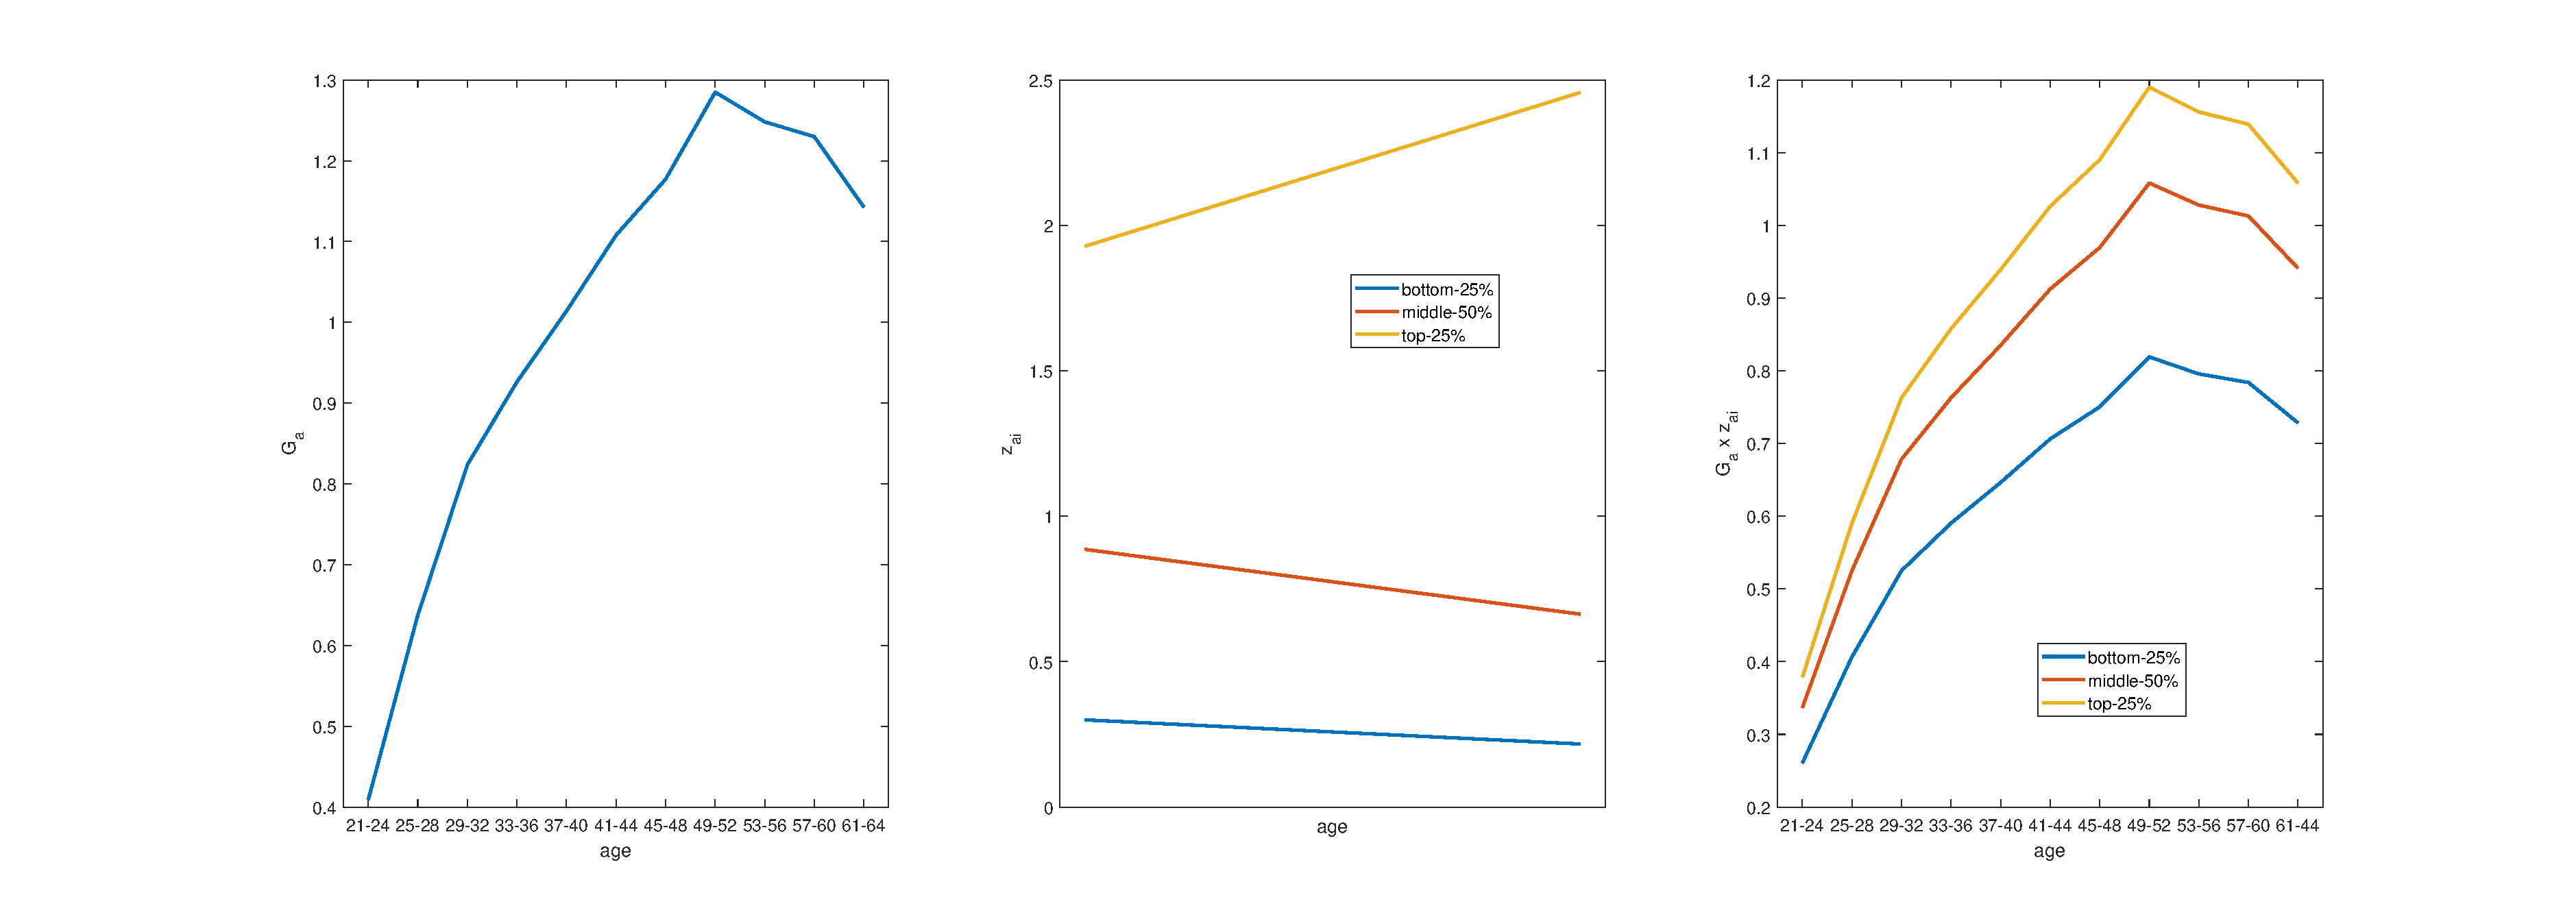
\includegraphics[width=18cm,height=8cm]{../Figures/IncomeProc.eps}
\end{center}
\end{figure}


In the model, we are calibrating each household's productivity. In the data, we do not observe productivity, but use earnings as our productivity estimate. If hours worked differed drastically across age and income groups, then the model's income distribution might look very different from that of the data. Hours worked are relatively flat across productivity and age, both in the model and in the data. Therefore, the model's (endogenous) income distribution looks similar to the data, as can be seen from the top panels of Figure \ref{Fig:WealthByAgeBaseline}.


\section{Housing Supply Elasticity calibration} \label{app:HSE}

We compute the long-run housing supply elasticity. It measures what happens to the housing quantity and housing investment in response to a 1\% permanent increase in house prices. Define housing investment as:
\[Y_t^h = \left(1-\frac{H_{t-1}}{\overline{H}}\right) N_{h,t}^{\rho_h}.\]
Note that $H_{t+1}=(1-\delta) H_t+Y_t^h$, so that in steady state, $Y^h=\delta H$. Rewriting the steady state housing investment equation in terms of equilibrium quantities using \eqref{eq:foclabor} delivers:
\[ H = \frac{1}{\delta} \left(1-\frac{H}{\overline{H}}\right)^\frac{1}{1-\rho_h}  \rho_h^{\frac{\rho_h}{1-\rho_h}}  {P}^{\frac{\rho_h}{1-\rho_h}} W^{\frac{-\rho_h}{1-\rho_h}}\]
Rewrite in logs, using lowercase letters to denote logs:
\[h = -\log(\delta) + \frac{1}{1-\rho_h} \log(1-\exp(h-\overline{h})) + \frac{\rho_h}{1-\rho_h} {p} - \frac{\rho_h}{1-\rho_h} w\]
Rearrange and substitute for $\overline p$ in terms of the market price $\overline p=\log(ho+(1-ho)\kappa_4)+p$:
\[p=  \frac{1-\rho_h}{\rho_h} h - \frac{1}{\rho_h} \log(1-\exp(h-\overline{h})) +  \frac{1-\rho_h}{\rho_h} \log(\delta) + w\]
Now take the partial derivative of $p$ w.r.t. $h$:
\[\frac{\partial p}{ \partial h} = \frac{1-\rho_h}{\rho_h} + \frac{1}{\rho_h} \frac{\exp(h-\overline{h})}{1-\exp(h-\overline{h})} + \frac{\partial w}{\partial h}\]
Invert this expression delivers the housing supply elasticity:
\[\frac{\partial h}{ \partial p} = \frac{\rho_h}{1-\rho_h + \frac{\exp(h-\overline{h})}{1-\exp(h-\overline{h})} + \rho_h \frac{\partial w}{\partial h}} \]
If the elasticity of wages to housing supply is small ($\frac{\partial w}{\partial h}\approx 0$), the housing supply elasticity simplifies to:
\[\frac{\partial h}{ \partial p} \approx \frac{\rho_h}{1-\rho_h + \frac{\exp(h-\overline{h})}{1-\exp(h-\overline{h})} } \]
We will use this approximation to calibrate the housing supply elasticity to the data. Since, in equilibrium, $Y^h=\delta H$, $\partial y^h/\partial p=\partial h/\partial p$.


Note that $h-\overline{h}$ measures how far the housing stock is from the constraint, in percentage terms. As $H$ approaches $\overline{H}$, the term $\frac{\exp(h-\overline{h})}{1-\exp(h-\overline{h})}$ approaches $+ \infty$ and the elasticity approaches zero.  If $H$ is far below $\overline{H}$, that term is close to zero and the housing supply elasticity is close to $\frac{\rho_h}{1-\rho_h}$.

In the baseline calibration, $\rho_h={\RTSC}$, $H/\overline{H}= {\HoverHbar}$ and $\frac{\partial w}{\partial h}=0.25$. The latter is calculated as the percentage change in wages divided by the percentage change in housing. These numbers deliver a house price elasticity of {\HSE}, close to the target of 1.0.

\section{Data Appendix} \label{app:data}

\subsection{The Typical U.S. Metropolitan Area}

We compile data on the largest 75 metropolitan statistical areas for the year 2016.  From the Census Bureau, we collect population for each MSA and each county. We also obtain data on the number of residents that are above age 65 and the number of residents that are above 21. Their ratio is the share of retirees. Finally, we obtain counts of the number of owner- and renter-occupied housing units, allowing us to construct the home ownership rate. From the American Community Survey, we obtain average commuting time and average property tax revenue.

From Zillow, we collect the Zillow House Value Index (ZHVI) and the Zillow Rental Index (ZRI) for each MSA and each county. The ZHVI is the price of a typical dwelling (single-family, condo, coop), while the ZRI is the monthly rent for a typical house (single-family, apartment). Zillow uses a machine-learning algorithm to control for property characteristics so that the resulting ZHVI and ZRI indices pertain to the \emph{same property} in a given period and location.

We match Census and Zillow data at the county level, which requires some manual work because of different naming conventions. The 75 MSAs are comprised of 487 counties. We split each MSA into two zones: the urban core, called zone 1, and the periphery containing the rest of the MSA, called zone 2. For the New York MSA, zone 1 is New York County (Manhattan), while for the Chicago MSA it is Cook County. For most MSAs (63 out of 75), zone 1 is a subdivision of a county (city) rather than an entire county. For example, Los Angeles county is far larger than the urban core, the city of Los Angeles. The same is true for Dallas County and Harris County in the Houston MSA. When using the county subdivisions, we collect data on population, income, retirees, owned and rented housing units, and property tax revenue from the ACS and prices and rents from Zillow for the constituent county subdivisions in order to allocate them to zone 1 and zone 2. We exclude the Greensboro MSA, the 75th largest MSA, since it consists of only one county. Our sample consists of the 74 largest MSA.

We then compute for all 74 MSAs the following 13 statistics: (1) MSA population, (2) MSA ZHVI $P$, (3) MSA ZRI $R$, (4) MSA price to annual rent ratio $P/R$, (5) the ratio of the msa population that is above age 65 to the msa population above age 21 ($reti$),  (6) the home ownership rate in the MSA ($Own$), (7) the average commuting time ($Commu$), (8) the ratio of retirees in zone 1 to zone 2 ($reti \, z1/z2)$, (9) the ratio of home ownership in zone 1 to zone 2 ($Own \, z1/z2$), (10) the ratio of ZRI in z1 to z2 ($R \, z1/z2$), (11) the ratio of income in zone 1 to zone 2 ($Inc \, z1/z2$), (12) the property tax rate in zone 1, calculated as average tax revenue divided by the average ZHVI ($tax\,z1$), (13) the same statistic in zone 2 ($tax \, z2$). Tables \ref{table:msas} and \ref{table:msas2} show these statistics for the largest 40 MSAs by population as well as the population-weighted average among all 74 MSAs.


We report 6 additional statistics which are (7)
Table \ref{table:msas2} shows these statistics for the largest 40 MSAs by population as well as the population-weighted average among all 75 MSAs.

\begin{table}
\caption{U.S. Metropolitan Area Statistics: Part 1}\label{table:msas}
\setlength{\tabcolsep}{5pt}
\renewcommand{\arraystretch}{1.05}
\begin{center}
{\scriptsize
    \begin{tabular}{lccccccc}
    \hline &  (1) & (2) & (3) & (4) & (5) & (6) & (7)\\
        \textbf{MSA name} & \textbf{Pop} & \textbf{P} & \textbf{R} & \textbf{P/R} & \textbf{reti} & \textbf{Own} & \textbf{Commu} \\     \hline
    New York & 20,153,634 & 498,955  &   2,404 & 17.30 & 19.1\% & 51.5\% & 36.3 \\
    Los Angeles-Long Beach-Anaheim &            13,310,447  &          557,640  &          2,587  & 17.96 & 17.1\% & 48.4\% & 30\\
    Chicago &               9,512,999  &          200,328  &          1,655  & 10.09 & 17.7\% & 64.2\% & 31.6\\
    Dallas-Fort Worth &               7,233,323  &          184,461  &          1,534  & 10.02 & 14.8\% & 59.7\% & 28.1 \\
    Houston &               6,690,766  &          179,457  &          1,575  & 9.49  & 14.2\% & 60.1\% & 29.7\\
    Washington &               6,131,977  &          398,394  &          2,194  & 15.13 & 15.6\% & 63.0\% & 34.6 \\
    Philadelphia &               6,070,500  &          203,562  &          1,590  & 10.67 & 19.7\% & 67.4\% & 29.5 \\
    Miami-Fort Lauderdale &               6,066,387  &          231,556  &          1,889  & 10.21 & 22.5\% & 60.1\% & 28.9\\
    Atlanta &               5,789,700  &          178,136  &          1,344  & 11.04 & 15.2\% & 63.0\% & 31.4 \\
    Boston &               4,794,447  &          410,340  &          2,296  & 14.90 & 19.2\% & 61.3\% & 31.0\\
    San Francisco &               4,679,166  &          829,218  &          3,389  & 20.39 & 18.3\% & 53.7\%& 32.8 \\
    Phoenix &               4,661,537  &          222,821  &          1,313  & 14.15 & 20.0\% & 61.4\% & 26.2\\
    Riverside &               4,527,837  &          308,608  &          1,704  & 15.09 & 17.3\% & 61.9\% & 32.1\\
    Detroit &               4,297,617  &          128,608  &          1,192  & 8.99  & 20.0\% & 68.6\% & 26.8\\
    Seattle &               3,798,902  &          418,325  &          2,072  & 16.83 & 16.5\% & 59.8\% & 30.1 \\
    Minneapolis-St Paul &               3,551,036  &          229,230  &          1,558  & 12.26 & 17.1\% & 69.7\% & 25.3\\
    San Diego &               3,317,749  &          509,700  &          2,431  & 17.47 & 17.4\% & 52.7\% & 25.7\\
    Tampa &               3,032,171  &          165,687  &          1,329  & 10.39 & 24.6\% & 63.9\% & 27.1\\
    Denver &               2,853,077  &          341,064  &          2,016  & 14.10 & 15.9\% & 63.3\% & 27.5 \\
    Baltimore &               2,798,886  &          240,402  &          1,766  & 11.35 & 19.0\% & 66.0\% & 30.8 \\
    St. Louis &               2,785,284  &          143,490  &          1,140  & 10.49 & 20.1\% & 69.0\% & 25.6\\
    Charlotte &               2,442,133  &          167,584  &          1,249  & 11.18 & 17.2\% & 65.3\% & 26.5\\
    Orlando &               2,441,257  &          188,415  &          1,380  & 11.38 & 18.8\% & 60.2\% & 28.2\\
    Portland &               2,424,955  &          342,224  &          1,774  & 16.08 & 17.9\% & 60.8\% & 26.6\\
    San Antonio &               2,380,812  &          163,058  &          1,320  & 10.30 & 17.4\% & 61.8\% & 26.0\\
    Sacramento &               2,296,418  &          343,465  &          1,688  & 16.96 & 19.3\% & 59.0\% & 26.8\\
    Las Vegas &               2,155,664  &          208,300  &          1,241  & 13.99 & 18.3\% & 52.3\% & 24.5\\
    Pittsburgh &               2,155,452  &          122,317  &          1,107  & 9.21  & 24.0\% & 69.2\% & 26.7\\
    Cincinnati &               2,142,179  &          140,438  &          1,263  & 9.27  & 19.0\% & 65.8\% & 24.7\\
    Austin &               2,056,405  &          266,196  &          1,735  & 12.79 & 13.3\% & 58.1\% & 26.8\\
    Cleveland &               2,055,612  &          122,949  &          1,163  & 8.81  & 22.4\% & 65.0\% & 24.6\\
    Columbus &               2,041,520  &          144,022  &          1,330  & 9.03  & 16.7\% & 61.1\% & 23.7\\
    Kansas City &               2,028,527  &          158,908  &          1,264  & 10.48 & 18.4\% & 64.7\% & 23.0\\
    Indianapolis &               2,004,230  &          139,160  &          1,211  & 9.58  & 17.4\% & 64.7\% & 24.8\\
    San Jose &               1,978,816  &          945,350  &          3,496  & 22.53 & 16.7\% & 56.7\% & 28.2 \\
    Nashville &               1,865,298  &          211,455  &          1,542  & 11.43 & 16.7\% & 65.3\% & 27.3\\
    Virginia Beach &               1,726,907  &          212,569  &          1,433  & 12.36 & 17.9\% & 61.0\% & 24.3\\
    Providence &               1,614,750  &          243,116  &          1,604  & 12.63 & 21.1\% & 60.5\% & 25.8\\
    Milwaukee &               1,572,482  &          178,678  &          1,302  & 11.43 & 19.2\% & 60.0\% & 23.1\\
    Jacksonville &               1,478,212  &          168,442  &          1,304  & 10.77 & 19.3\% & 64.5\% & 26.5 \\             \hline
    Pop-weighted avg 74 MSAs &  6,075,613 & 297,875 & 1,775 & 13.03 & 18.3\% & 60.6\%  &  28.64  \\
    %Equally-weighted avg 75 MSAs &  2,650,526 & 238,508 & 1,551 & 11.97 & 19.0\% & 63.1\%    \\
    \hline
    \end{tabular}%
    }
    \end{center}
  \end{table}%



\begin{table}
\caption{U.S. Metropolitan Area Statistics: Part 2}\label{table:msas2}
\setlength{\tabcolsep}{5pt}
\renewcommand{\arraystretch}{1.05}
\begin{center}
{\scriptsize
    \begin{tabular}{lcccccc}
    \hline &   (8) & (9) & (10) & (11) & (12) & (13) \\
        \textbf{MSA name} & \textbf{reti z1/z2} & \textbf{Own z1/z2} & \textbf{R z1/z2} & \textbf{Inc z1/z2} & \textbf{tax z1} & \textbf{tax z2}  \\     \hline
New York &    0.91  & 0.42  & 1.68  & 2.70  & 0.55\% & 1.89\%  \\
Los Angeles-Long Beach-Anaheim &0.87  & 0.68  & 1.06  & 0.91  & 0.89\% & 0.87\%  \\
Chicago&0.81  & 0.61  & 1.03  & 0.92  & 2.05\% & 3.06\%  \\
Dallas-Fort Worth & 0.90  & 0.65  & 0.87  & 1.00  & 3.15\% & 2.17\%  \\
Houston & 0.96  & 0.61  & 0.88  & 0.88  & 2.62\% & 2.32\%  \\
Washington & 0.93  & 0.62  & 1.19  & 1.16  & 0.81\% & 1.19\%  \\
Philadelphia & 0.83  & 0.72  & 0.72  & 0.85  & 1.27\% & 1.50\%  \\
Miami-Fort Lauderdale & 0.92  & 0.49  & 1.16  & 0.69  & 1.60\% & 2.27\%  \\
Atlanta & 0.94  & 0.66  & 1.08  & 1.48  & 2.20\% & 1.25\%  \\
Boston & 0.70  & 0.53  & 1.12  & 1.01  & 0.86\% & 1.47\%  \\
San Francisco & 0.92  & 0.63  & 1.44  & 1.40  & 0.89\% & 0.75\%  \\
Phoenix &  0.62  & 0.80  & 0.93  & 0.90  & 0.63\% & 0.85\%  \\
Riverside & 0.84  & 0.87  & 1.03  & 0.98  & 0.85\% & 1.05\%  \\
Detroit & 0.88  & 0.67  & 0.59  & 0.48  & 2.86\% & 2.19\%  \\
Seattle & 0.87  & 0.73  & 1.25  & 1.22  & 0.82\% & 1.08\%  \\
Minneapolis-St Paul & 0.66  & 0.65  & 0.97  & 0.95  & 1.64\% & 1.40\%  \\
San Diego & 0.86  & 0.81  & 1.01  & 1.06  & 0.86\% & 0.91\%  \\
Tampa &  0.63  & 0.73  & 0.99  & 1.04  & 1.85\% & 1.24\%  \\
Denver & 0.87  & 0.72  & 0.98  & 1.26  & 0.62\% & 0.70\%  \\
Baltimore & 0.84  & 0.65  & 0.71  & 0.78  & 3.73\% & 1.29\%  \\
St. Louis &    0.73  & 0.59  & 0.76  & 0.81  & 1.53\% & 1.87\%  \\
Charlotte & 0.68  & 0.74  & 1.05  & 1.18  & 1.72\% & 1.08\%  \\
Orlando &      0.69  & 0.56  & 0.92  & 0.90  & 1.36\% & 1.17\%  \\
Portland & 0.78  & 0.83  & 1.05  & 1.05  & 2.19\% & 1.84\%  \\
San Antonio & 0.86  & 0.72  & 0.86  & 0.77  & 1.12\% & 1.11\%  \\
Sacramento & 0.84  & 0.75  & 0.85  & 0.83  & 2.22\% & 2.39\%  \\
Las Vegas & 1.08  & 1.00  & 0.99  & 0.98  & 1.02\% & 0.97\%  \\
Pittsburgh & 0.73  & 0.65  & 1.05  & 0.89  & 0.90\% & 0.86\%  \\
Cincinnati & 0.83  & 0.53  & 0.81  & 0.81  & 2.83\% & 1.96\%  \\
Austin &   0.68  & 0.64  & 1.09  & 1.12  & 1.90\% & 1.52\%  \\
Cleveland & 0.77  & 0.59  & 0.68  & 0.56  & 1.97\% & 2.14\%  \\
Columbus & 0.67  & 0.61  & 0.77  & 0.75  & 2.34\% & 2.43\%  \\
Kansas City & 0.87  & 0.79  & 0.76  & 0.84  & 3.91\% & 2.51\%  \\
Indianapolis & 0.83  & 0.72  & 0.83  & 0.94  & 1.41\% & 1.18\%  \\
San Jose & 0.89  & 1.01  & 0.94  & 0.78  & 0.79\% & 0.74\%  \\
Nashville & 0.81  & 0.74  & 0.99  & 1.19  & 1.08\% & 0.74\%  \\
Virginia Beach & 0.91  & 1.05  & 1.10  & 1.19  & 1.07\% & 1.14\%  \\
Providence & 0.61  & 0.54  & 0.88  & 0.76  & 2.77\% & 1.66\%  \\
Milwaukee &  0.64  & 0.59  & 0.66  & 0.58  & 3.57\% & 1.99\%  \\
Jacksonville & 0.76  & 0.78  & 0.76  & 0.80  & 1.37\% & 1.23\%  \\ \hline
Pop-weighted avg 74 MSAs &  0.84 & 0.65 & 1.03 & 1.12 & 1.60\% & 1.57\%    \\
%Equally-weighted avg 74 MSAs &  0.84 & 0.69 & 0.93 & 0.93 & 1.82\% & 1.50\%    \\
\hline
    \end{tabular}%
    }
    \end{center}
  \end{table}%



\subsection{Out-of-town Housing Demand} \label{app:corelogic}
Out-of-town (OOT) housing demand is estimated using the data set compiled for us by {\tt CoreLogic}. This confidential data set contains the monthly time series of number of housing purchases for Manhattan and for NYC MSA between January 2004 and September 2016. Housing purchases are defined as purchases of single-family, 2-4 family, condominiums, and co-ops. OOT purchases are identified using the reported mailing addresses on payment/tax forms. Specifically, if the address of a buyer is either abroad or not contained in the list of 1,304 ZIP codes inside NYC MSA, then the transaction is classified as an OOT purchase.


One complication arises because not only individuals but also companies purchase residential real estate. We include purchases by the following types of corporate entities: LLC, Inc, Corp, and Trust. Combined, these account for 7.28\% of all purchases in the New York metro and even 11.13\% in Manhattan. We have an address for these corporate purchases as well. Following the same address rules, we obtain the number of OOT corporate purchases and the number of NY MSA corporate purchases in each month. If the buyer of an apartment is a corporation, we can not be certain whether the individual who ultimately owns the apartment is a local or from OOT. Some OOT corporate purchases may be done by locals while some NY MSA corporate purchases may actually hide the identity of OOT investors. Under \emph{assumption 1}, we assume that all OOT corporate purchases are by OOT investors and none of the NY MSA corporate purchases are by OOT buyers. Under \emph{assumption 2}, we assume that 70\% of all OOT corporate purchases are by OOT investors and 30\% of the NY MSA corporate purchases are by OOT buyers. We have also computed the OOT share assuming (90\%,10\%) and (80\%,20\%) assumptions and the results are in between those for assumption 1 and assumption 2. Since there are a lot more NY MSA corporate purchases than OOT corporate purchases, the OOT share under assumption 2 is higher than under assumption 1.

As described in Table \ref{tab:OOTNYdata}, the average OOT purchase fractions are 9.2\%/2.8\% for Manhattan/Rest of NY metro under \textit{assumption 1}, while the fractions are 11.6\%/4.6\% under \textit{assumption 2}. Based on conversations with market participants, we believe assumption 2 comes closer to approximating the true OOT share. A full-sample OOT share of 5\% for the entire NYC metro area and of 10\% for Manhattan seem conservative (Panel C).

\begin{table}[htbp]
  \caption{Fraction of OOT Purchases of New York Housing Units}
\setlength{\tabcolsep}{4pt}
\renewcommand{\arraystretch}{1.05}
\begin{center}
{\scriptsize
    \begin{tabular}{|l|c|ccc|}
    \hline
    \multicolumn{5}{|c|}{\textbf{Panel A: Manhattan}} \\     \hline
    \textbf{Assumption} & \textbf{2004.01-2016.09} & \multicolumn{1}{c}{2004.01 - 2007.12} & \multicolumn{1}{c}{2008.01 - 2011.12} & 2012.01 - 2016.09  \\    \hline
     1 & 9.2\%  & 8.2\% & 9.0\% & 10.1\%  \\
     2 & 11.6\% & 9.6\% & 11.4\% & 13.4\%  \\     \hline
    \multicolumn{5}{|c|}{\textbf{Panel B: Rest of New York metro area}} \\     \hline
     1 & 2.8\%  & 2.5\% & 2.6\% & 3.1\%  \\
     2 & 4.6\%  & 3.6\% & 4.4\% & 5.8\%  \\
         \hline
    \multicolumn{5}{|c|}{\textbf{Panel C: New York metro area}} \\     \hline
     1 & 3.3\%  & 2.9\% & 3.3\% & 3.8\%  \\
     2 & 5.3\%  & 4.0\% & 5.0\% & 6.5\%  \\
         \hline
        \end{tabular}
}
\end{center}
\begin{minipage}{\textwidth}\tiny
    \smallskip{\it Notes:} Share of  residential real estate purchases made by out-of-town (OOT) buyers in the New York metropolitan area. Source: Core Logic. Monthly data from January 2004 through September 2016.
    \end{minipage}
  \label{tab:OOTNYdata}%
\end{table}%

\subsection{Migration} \label{app:dataNYC_migration}

We use county-to-county migration data for 2006-2010 and 2010-2014 from the 5-year American Community Survey for the 25 counties in the New York metropolitan area. For each county and survey wave, we compute net migration rates (inflow minus outflow divided by population). When one person enters the New York labor market and another one leaves, the model is unchanged, so net migration is the relevant concept for the model. We aggregate net migration for the 24 counties other than Manhattan and call them zone 2. The net migration rate over the 5-year period between 2010-2014 for the entire MSA is -0.15\%, or -0.03\% per year. First, this net migration rate is minuscule: only about 30,000 people moved in over a 5-year period on a MSA population of 20 million. Of course, this masks much larger gross flows: about 824,000 came into the MSA and 854,000 left. Second, Manhattan saw a net inflow of 30,000 people coming from outside the MSA while the rest of the MSA (zone 2) saw a net outflow to the rest of the country/world of 60,000. This is the opposite pattern than what we would expect if the OOT purchases prompted migration of residents, since OOT purchases were much stronger in Manhattan than in the rest of the MSA (twice as large). Third, comparing the net migration in the 2010-2014 period to that in the 2006-2010 period, we find that the net migration rate rose, from -73,000 to -30,000. The net migration rate rises from -0.38\% in 2006-2010 to -0.15\% in the 2010-2014 period. The rise in OOT purchases over time did not coincide with a decline in net migration, but with an increase. In other words, not only are the relevant net migration rates tiny, they also have the wrong-sign cross-sectional correlation with the spatial OOT pattern, and with the time-series of OOT purchases. We conclude that there is little evidence in the New York data of substantial net migration responses to OOT purchases.


\end{small}
\end{spacing}

\end{document}


%Fourth, the modeling of an outside option value is much more complicated in a life-cycle model. A 30-, 50-, and 70-year old in the model have vastly different value functions. When confronted with the same outside option and moving cost, they would make vastly different moving decisions. This would either lead to counter-factual moving patterns or necessitate a highly parameterized outside option-minus-moving cost function, for which the literature provides little guidance. The exercise would quickly become arbitrary. For these four reasons, we do not believe it is fruitful to explore this route further.



%%%%%%%%%%%%%%%%%%%%%%%%%%%%%
%
%
%             Vancouver Data Appendix
%
%
%
%%%%%%%%%%%%%%%%%%%%%%%%%%%%%

\subsection{Data Appendix: Vancouver} \label{app:dataVancouver}

\subsubsection{The Vancouver Metro Area}
{\tt{Statistics Canada}} (\url{http://www.statcan.gc.ca}) publishes the list and delineations of Census Metropolitan Areas (CMAs) as a part of the national Census program every five years. Vancouver CMA is the third most populous CMA in Canada, after the Toronto CMA and the Montreal CMA. We use the latest definition of Vancouver CMA from the 2011 Census Program. Vancouver CMA consists of 39 Census subdivisions (CSDs): 12 cities, 5 district municipalities, 3 villages, 1~RDA (Regional District Electoral Area), 1 island municipality, and 17 Indian reserves. Among these, we include cities, district municipalities, villages and the RDA in our definition of the Vancouver Metro Area. We use the terms CSDs and municipalities interchangeably hereafter.

The city of Vancouver is defined as zone 1, and zone 2 includes the rest 20 CSDs. Table \ref{Tbl:VancouverCMA} exhibits the complete list of CSDs and their types in our Vancouver Metro Area zoning definitions.

\begin{table}[ht]\caption{Vancouver CMA}\label{Tbl:VancouverCMA}
        \centering
        \begin{tabular}{l c c}\hline\hline
                \textbf{Census Subdivision} & \textbf{CSD Type} & \textbf{Zone} \\ \hline
                Vancouver & City & Zone 1\\ \hline
                Burnaby & City & Zone 2 \\
                Coquitlam & City & Zone 2 \\
                Langley & City & Zone 2 \\
                New Westminster & City & Zone 2 \\
                North Vancouver & City & Zone 2 \\
                Pitt Meadows & City & Zone 2 \\
                Port Coquitlam & City & Zone 2 \\
                Port Moody & City & Zone 2 \\
                Richmond & City & Zone 2\\
                Surrey & City & Zone 2\\
                White Rock & City & Zone 2\\
                Delta & District Municipality & Zone 2\\
                Langley & District Municipality & Zone 2\\
                Maple Ridge & District Municipality & Zone 2\\
                North Vancouver & District Municipality & Zone 2\\
                West Vancouver & District Municipality & Zone 2 \\
                Anmore & Village & Zone 2 \\
                Belcarra & Village & Zone 2 \\
                Lions Bay & Village & Zone 2 \\
                Greater Vancouver A & RDA & Zone 2 \\
                \hline
        \end{tabular}
\end{table}


\subsubsection{Population, Housing Stock, and Land Area} \label{app:dataVancouver_pop}

The main source for population, housing stock, and land area is the {\tt{2011 Census}} published by Statistics Canada (\url{http://www12.statcan.gc.ca/census-recensement/index-eng.cfm}). From the webpage, the name of  CSDs can be queried with an additional option to select the data source; the 2011 Census or the 2011 NHS (National Household Survey). After retrieving all the data at the CSD level, we aggregate data into zone 1 and zone 2 level data.

Population, housing stocks and land area are all reported in \textit{Population and dwelling counts} section. For housing stocks, the Census distinguishes between \textit{Total dwellings} and \textit{Private dwellings occupied by usual residents}, to account for vacancies. We ignore the vacancies and only use \textit{Private dwellings occupied by usual residents}, which is also equivalent to \textit{Total number of private households} in 2011 NHS. Additionally, the \textit{Age characteristics} section gives details of age distributions, from which we can estimate the average age in each zone as well as the fraction of the population above 65 conditional on being above 21.

%2016 Census survey has been completed but the data is scheduled to be released sequentially, and the complete data will be publicly available only at the end of 2017 (http://www12.statcan.gc.ca/census-recensement/ 2016/ref/release-dates-diffusion-eng.cfm).

Greater Vancouver A (RDA) includes several unincorporated areas in the region, and it contains the vast and unpopulous land in the northern end of the Vancouver CMA. We assume that all the reported population for Greater Vancouver A are living in UEL (University Endowment Land) -- the area containing the University of British Columbia --  and override the Greater Vancouver A land area (815.59km$^2$) with the UEL land area (14.13km$^2$).


\subsubsection{Income}

The main source for income distribution is {\tt{2011 NHS}} (National Household Survey) by Statistics Canada. The CSD-level data can be retrieved by following the same procedure as described in the previous section for 2011 Census program. In the \textit{Income of households in 2010} section of 2011 NHS, the detailed household income distribution is reported.

Since the housing prices and rent prices are all based on 2016 dollars, there is a discrepancy between the timing of income data and price data. The easiest way to correct this would be to use 2016 Census data. However, although the 2016 Census survey has been completed, the data is not publicly available yet. Statistics Canada will sequentially release the 2016 Census data according to the posted schedule (\url{http://www12.statcan.gc.ca/census-recensement/2016/ref/release-dates-diffusion-eng.cfm}), and the entire data will be released only at the end of 2017.

Instead, we make an adjustment to income level by using aggregate labor income growth. To this end, we use Table 111-0024 in {\tt{CANSIM}} database by Statistics Canada, which shows that the average labor income of tax filers with labor income grew by 11\% between 2010 and 2014. (\url{http://www5.statcan.gc.ca/cansim/a26?lang=eng\&retrLang=eng\&id=1110024}). By scaling it up to estimate the six-year growth, we estimate that there has been 17\% increase in labor income between 2010 and 2016. We assume that all the households have experienced the same income growth by 17\%, i.e. we are effectively scaling up the endpoints of income brackets by 17\%, without altering the distribution.

To aggregate the CSD-level income distribution into a zone 2 income distribution, we follow the same procedure as described in Appendix \ref{app:dataNYC}, Section \ref{app:dataNYC_income} for the New York MSA.


\subsubsection{House Prices, Rental Prices, and Home Ownership} \label{app:dataVancouver_pxrent}

Home ownership rate can be easily calculated from 2011 NHS data (\url{http://www12.statcan.gc.ca/ census-recensement/index-eng.cfm}). Under the \textit{Household characteristics} section, the \textit{Total number of private households by Tenure} is divided into \textit{Owners} and \textit{Renters}.

The main source for housing prices in Vancouver Metro Area is the \textit{Metro Vancouver Housing Data Book} (``MVHDB'') published by {\tt{Metro Vancouver}} (\url{http://www.metrovancouver.org/services/ regional-planning/PlanningPublications/MV\_Housing\_Data\_Book.pdf}) revised as of December 2016. Pages 105-107 of MVHDB contain three tables presenting house price information across municipalities, one for each category of housing (single-detached, semi-detached and rowhouse, apartment). These are compilations of survey data originally from \textit{Real Estate Board of Greater Vancouver} (REBGV) and \textit{Fraser Valley Real Estate Board} (FVREB). On page 17  of MVHDB, the number of housing units in each category is presented, which can be easily reproduced from the 2011 Census \textit{Household and dwelling characteristics} section. Using the number of housing units in each category as weights, we calculate a weighted-average house price for each municipality.

In reporting house prices, {\tt{REBGV}} uses a slightly different geographical division from Census CSDs. The city of Vancouver is further divided into Vancouver East and Vancouver West, and Delta is further divided into Delta(north) and Ladner-Delta(South). Since Census 2011 and NHS 2011 do not distinguish between these sub-areas, we use a different source to further divide the city of Vancouver and Delta housing numbers. {\tt{The Globe and Mail House Price Data Center}} (\url{http://www.theglobeandmail.com/real-estate /house-price-data-centre-toronto-propels-house-prices-to-new-record/article29697029/}) provides a detailed housing sales volume data and average sales price data at the zip code level. We define the following 15 zip codes as Vancouver West: V5Y, V5Z, V6B, V6C, V6E, V6G, V6H, V6J, V6K, V6L, V6M, V6N, V6P, V6R, V6Z. The rest 12 zip codes of the city of Vancouver (V5K, V5L, V5M, V5N, V5P, V5R, V5S, V5T, V5V, V5W, V5X, V6A) are defined as Vancouver East. Since there were 1,289 sales in 2016 Q2 in Vancouver East, and 2,635 sales in Vancouver West, for each category we allocate roughly 67\% of housings to Vancouver West, and the rest to Vancouver East. Similarly, we define V4C and V4E as Delta(north), while V4K, V4L and V4M are classified as Ladner-Delta(south) sub-area. Since there were 357 and 349 sales in Delta(south) and Delta(north) during 2016 Q2, respectively, for each category we allocate 51 \% of housings to Delta(north) and the rest into Ladner-Delta(south).

The main source for rental price data is \textit{2016 Rental Market Report for Vancouver CMA} published by {\tt{Canada Mortgage and Housing Corporation}} (\url{https://www.cmhc-schl.gc.ca/odpub
/esub/64467/64467\_2016\_A01.pdf?lang=en}). From the \textit{CMHC Report}, we use Table 1.1.2 for private apartment average rents and Table 1.1.3 for the number of private apartment units across municipalities. Zone 2 aggregate rent level is the weighted-average rent using the number of private apartment units as weights. Note that Table 1.1.3 is also reproduced in MVHDB on page 82. When the number of private apartments in two or more municipalities are reported as an aggregate (for example, ``Tri-cities'' -- Coquitlam, Port Moody and Port Coquitlam -- are reported as a group) we allocate the aggregated private apartment number into each municipality, using 2011 NHS \textit{renters} as weights. Private apartments account for about 38\% of the entire rental units in the region -- there are also secondary suites, non-market rental units and privately rented condominium units (see p. 45 of MVHDB). However, since private apartments are considered as the primary rental market, we use these numbers as the benchmark rental prices.




\end{small}
\end{spacing}

\end{document}


